\documentclass{aa}  
\usepackage{graphicx}
\usepackage{txfonts}
\usepackage{hyperref}
\usepackage{color}
\usepackage{float}

\begin{document} 


   \title{Magnetized accretion disks around Kerr black holes with scalar hair}

%   \subtitle{}

\author{Sergio Gimeno-Soler\inst{1}, Jos\'e A.~Font\inst{1,2}, Carlos Herdeiro \inst{3}, Eugen Radu\inst{3}}
\institute{Departamento de Astronom\'{\i}a y Astrof\'{\i}sica, Universitat de Val\`encia, Dr. Moliner 50, 46100, Burjassot (Val\`encia), Spain.\\\email{sergio.gimeno@uv.es}
\and
Observatori Astron\`omic, Universitat de Val\`encia, C/ Catedr\'atico Jos\'e Beltr\'an 2, 46980, Paterna (Val\`encia), Spain. \\
\email{j.antonio.font@uv.es}
\and
Departamento de F\'isica da Universidade de Aveiro and Centre for Research and Development in Mathematics and Applications (CIDMA), Campus de Santiago, 3810-183 Aveiro, Portugal
}

% \abstract{}{}{}{}{} 
% 5 {} token are mandatory

  \date{}
 
  \abstract
  {We present a method to build magnetized constant angular momentum disks around Kerr black holes with scalar hair (KBHsSH).}

   \keywords{black hole physics
               }

   \maketitle
%
%-------------------------------------------------------------------

\section{Introduction}

% Outline: 

% Brief description of the work of Herdeiro, recall what we use here and proceed to describe what we have done.
% First, describe framework. Metric, energy-momentum tensor, and equations of motion. Second, angular momentum distribution (including the angular momentum at $r_{\mathrm{mb}}$) and EoS. Third, results: Higher potential well than any possible Kerr-like solution with $r_{\mathrm{in}} = r_{\mathrm{mb}}$. We should graph here the potential well $\Delta W$ vs. the normalized spin parameter $a$ for the KBH case. Maybe get the data for intermediate values of magnetization? I think it is important to have more data of HBH, to test some ideas. Comparison with naked singularities? I would like to obtain the rest-mass and gravitational mass of the total distribution (torus + scalar field).

% Comparison of the structure of the disks obtained for the case of KBHsSH with KBH and Naked Singularities (NS). $\Delta W$, angular velocity, angular momentum, mass of the torus and physical magnitudes (thermodynamical)

% Paint same curves (if possible) as in the case of the previous paper for magnetized toris around KBHs, check differences between the cases. For KBHs with full-relativistic fluid and HBHs.

% Check relations between ergoregions in KBHs and NSs spacetimes and KBHsSH case (morphology?)
% The most important conclusion is we obtain very different disk configurations for HBHs and for KBHs (with the same ADM or Horizon quantities), therefore we can asymptotically distinguish a disk around a KBHsSH from a disk around a KBH. (potential well and so on).

%--------------------------------------------------------------------
\section{Framework}

We use the stationary and axisymmetric metric ansatz provided by\citet{Herdeiro:2014a}

\begin{equation}
\mathrm{d}s^2 = e^{2F_1}\left(\frac{\mathrm{d}r^2}{N} + r^2\mathrm{d}\theta^2\right) + e^{2F_2}r^2\sin^2 \theta(\mathrm{d}\phi-W\mathrm{d}t)^2-e^{2F_0}N\mathrm{d}t^2,
\end{equation}

with $N = 1 - r_H/r$, where $r_H$ is the radius of the event horizon of the BH and $W$, $F_1$, $F_2$, $F_0$ are functions of $r$ and $\theta$.

\begin{figure*}
\centering
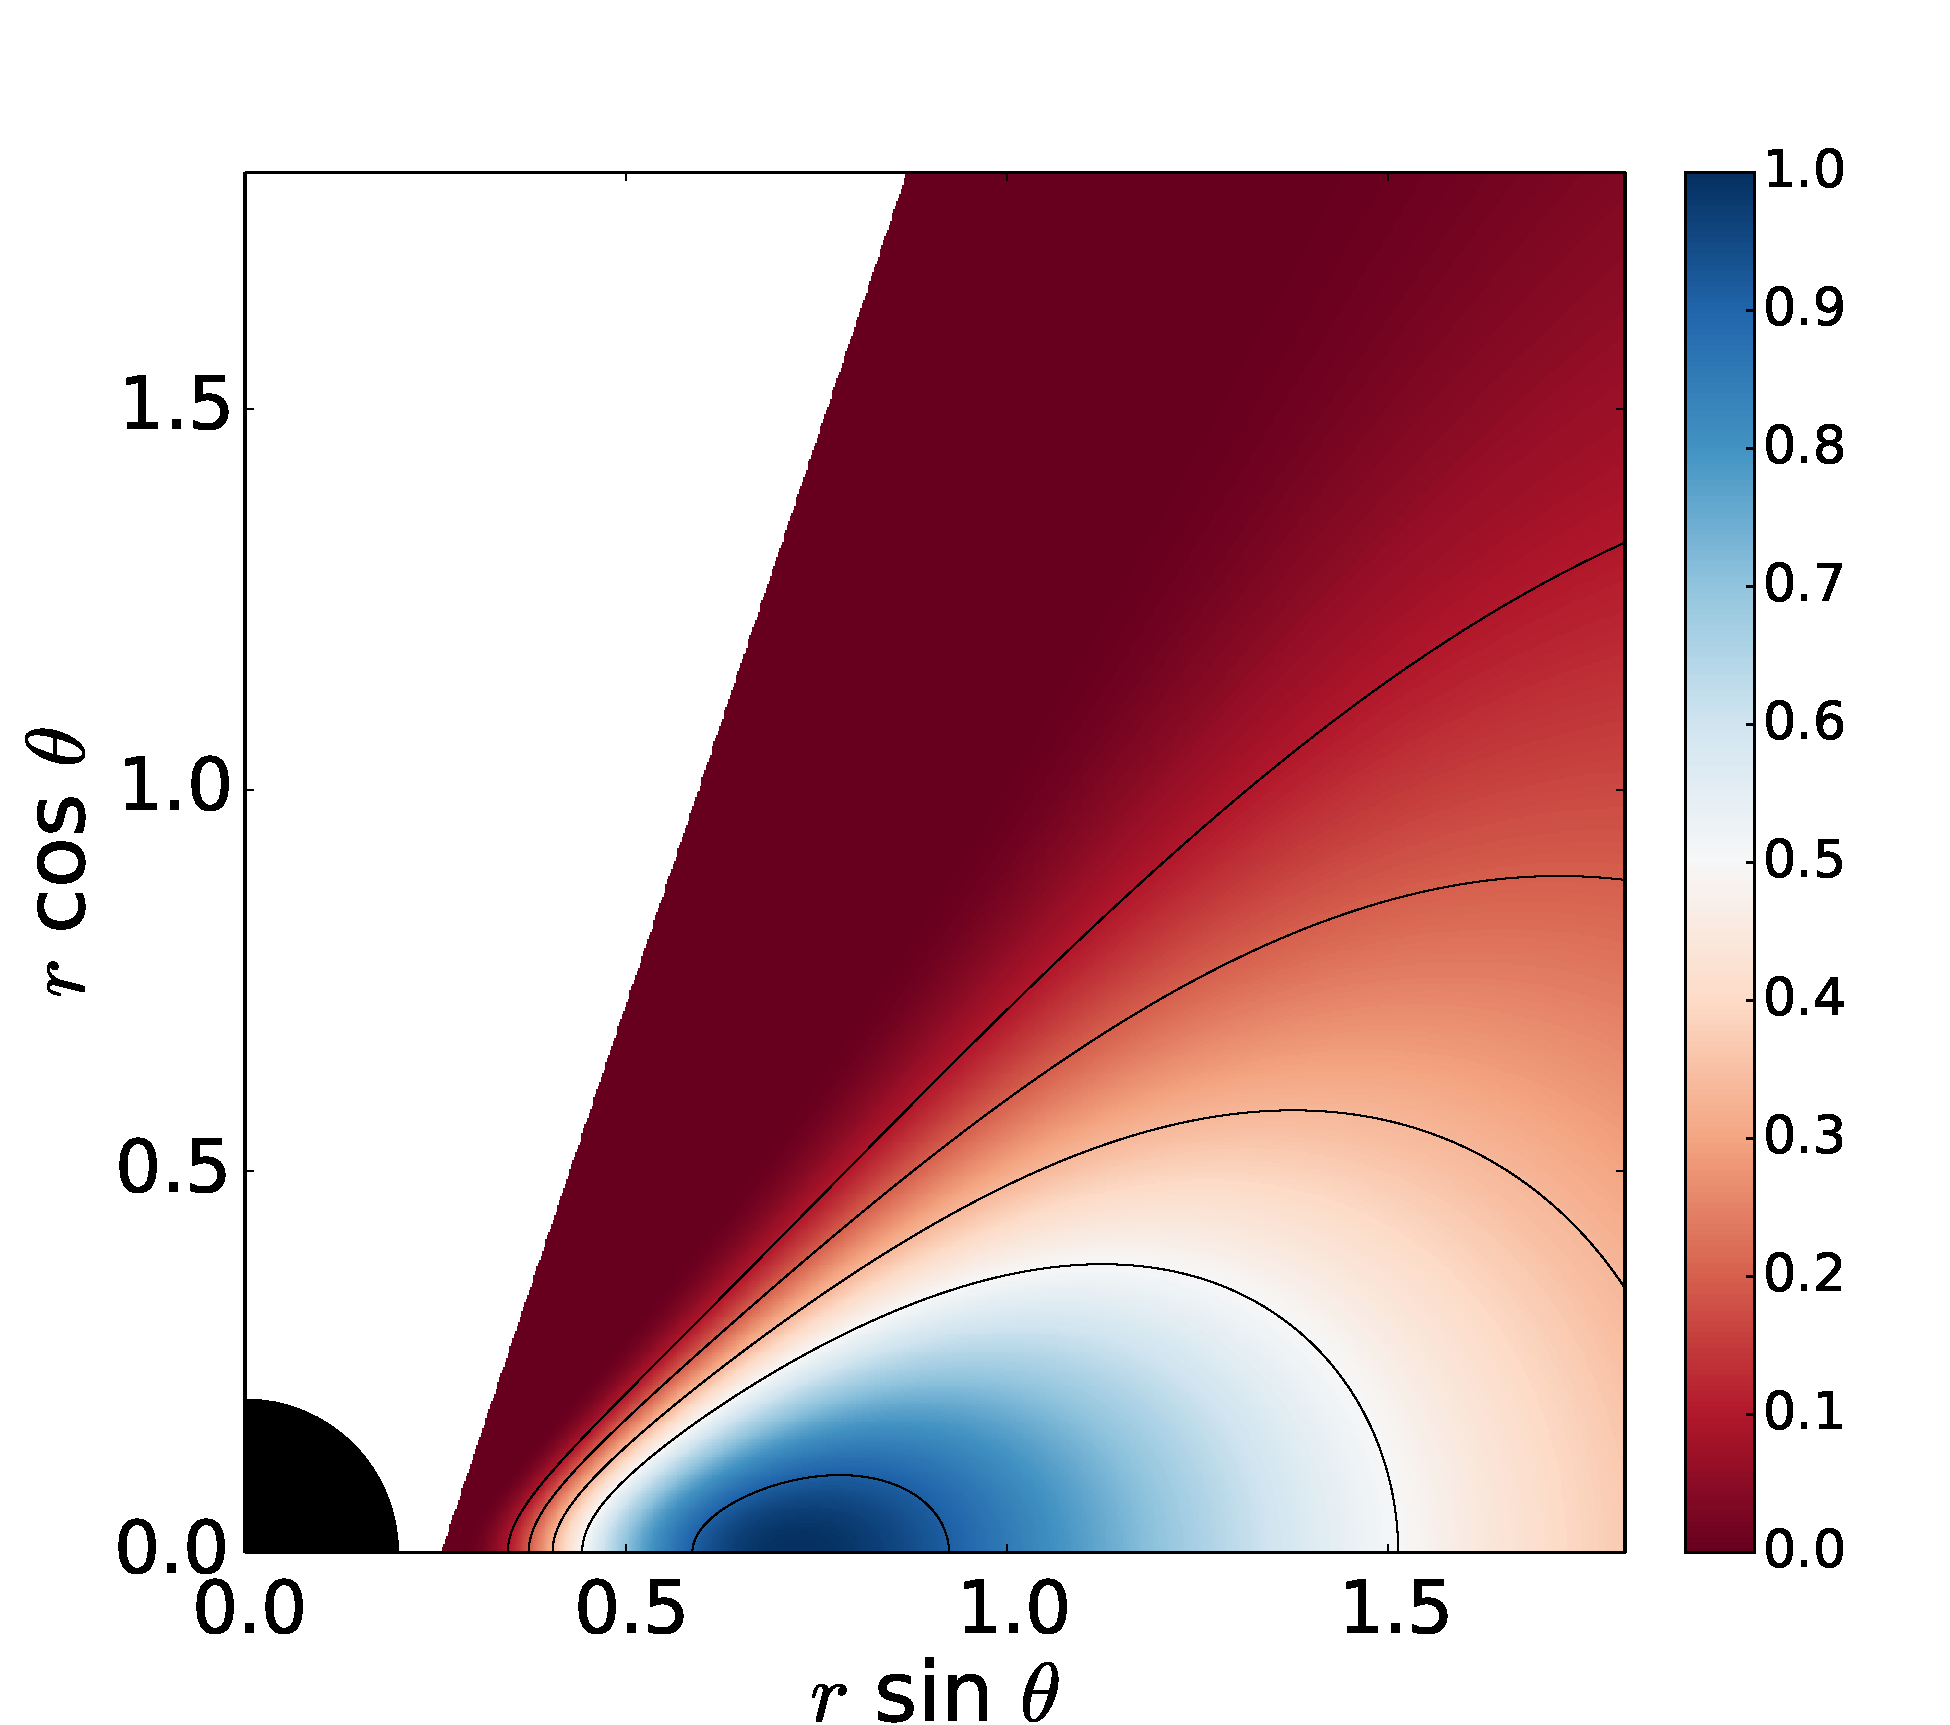
\includegraphics[scale=0.14]{figures/fig1_III_3.pdf}
\hspace{-0.3cm}
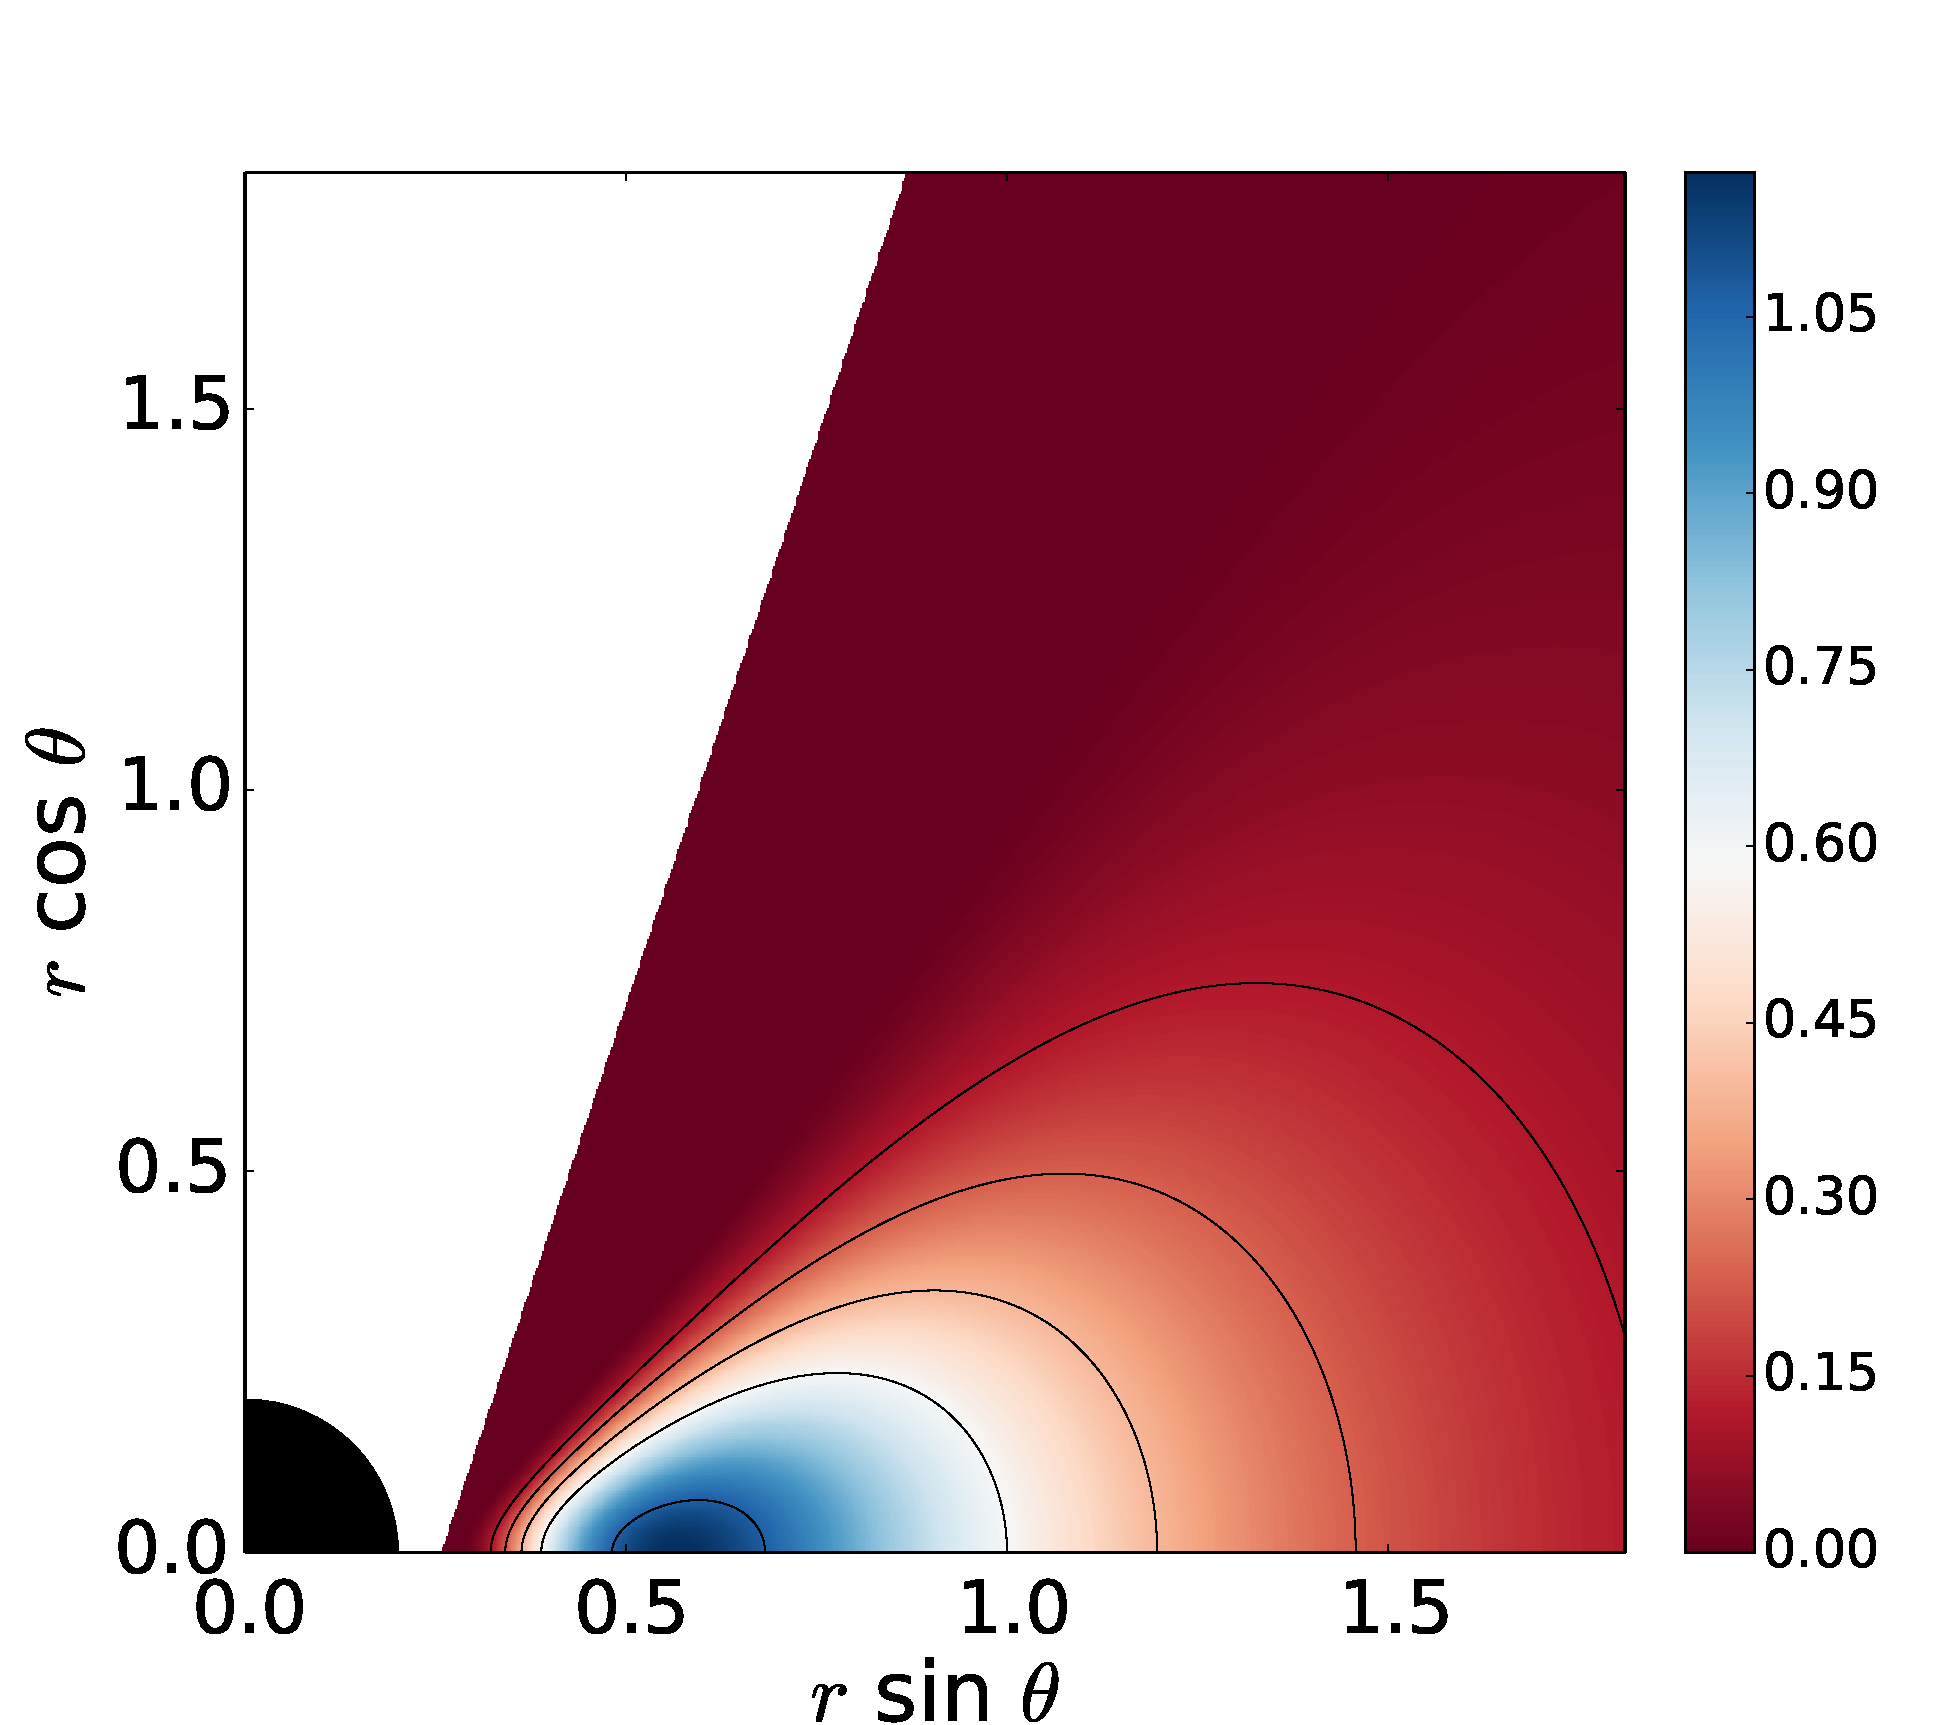
\includegraphics[scale=0.14]{figures/fig1_III_0.pdf}
\hspace{-0.2cm}
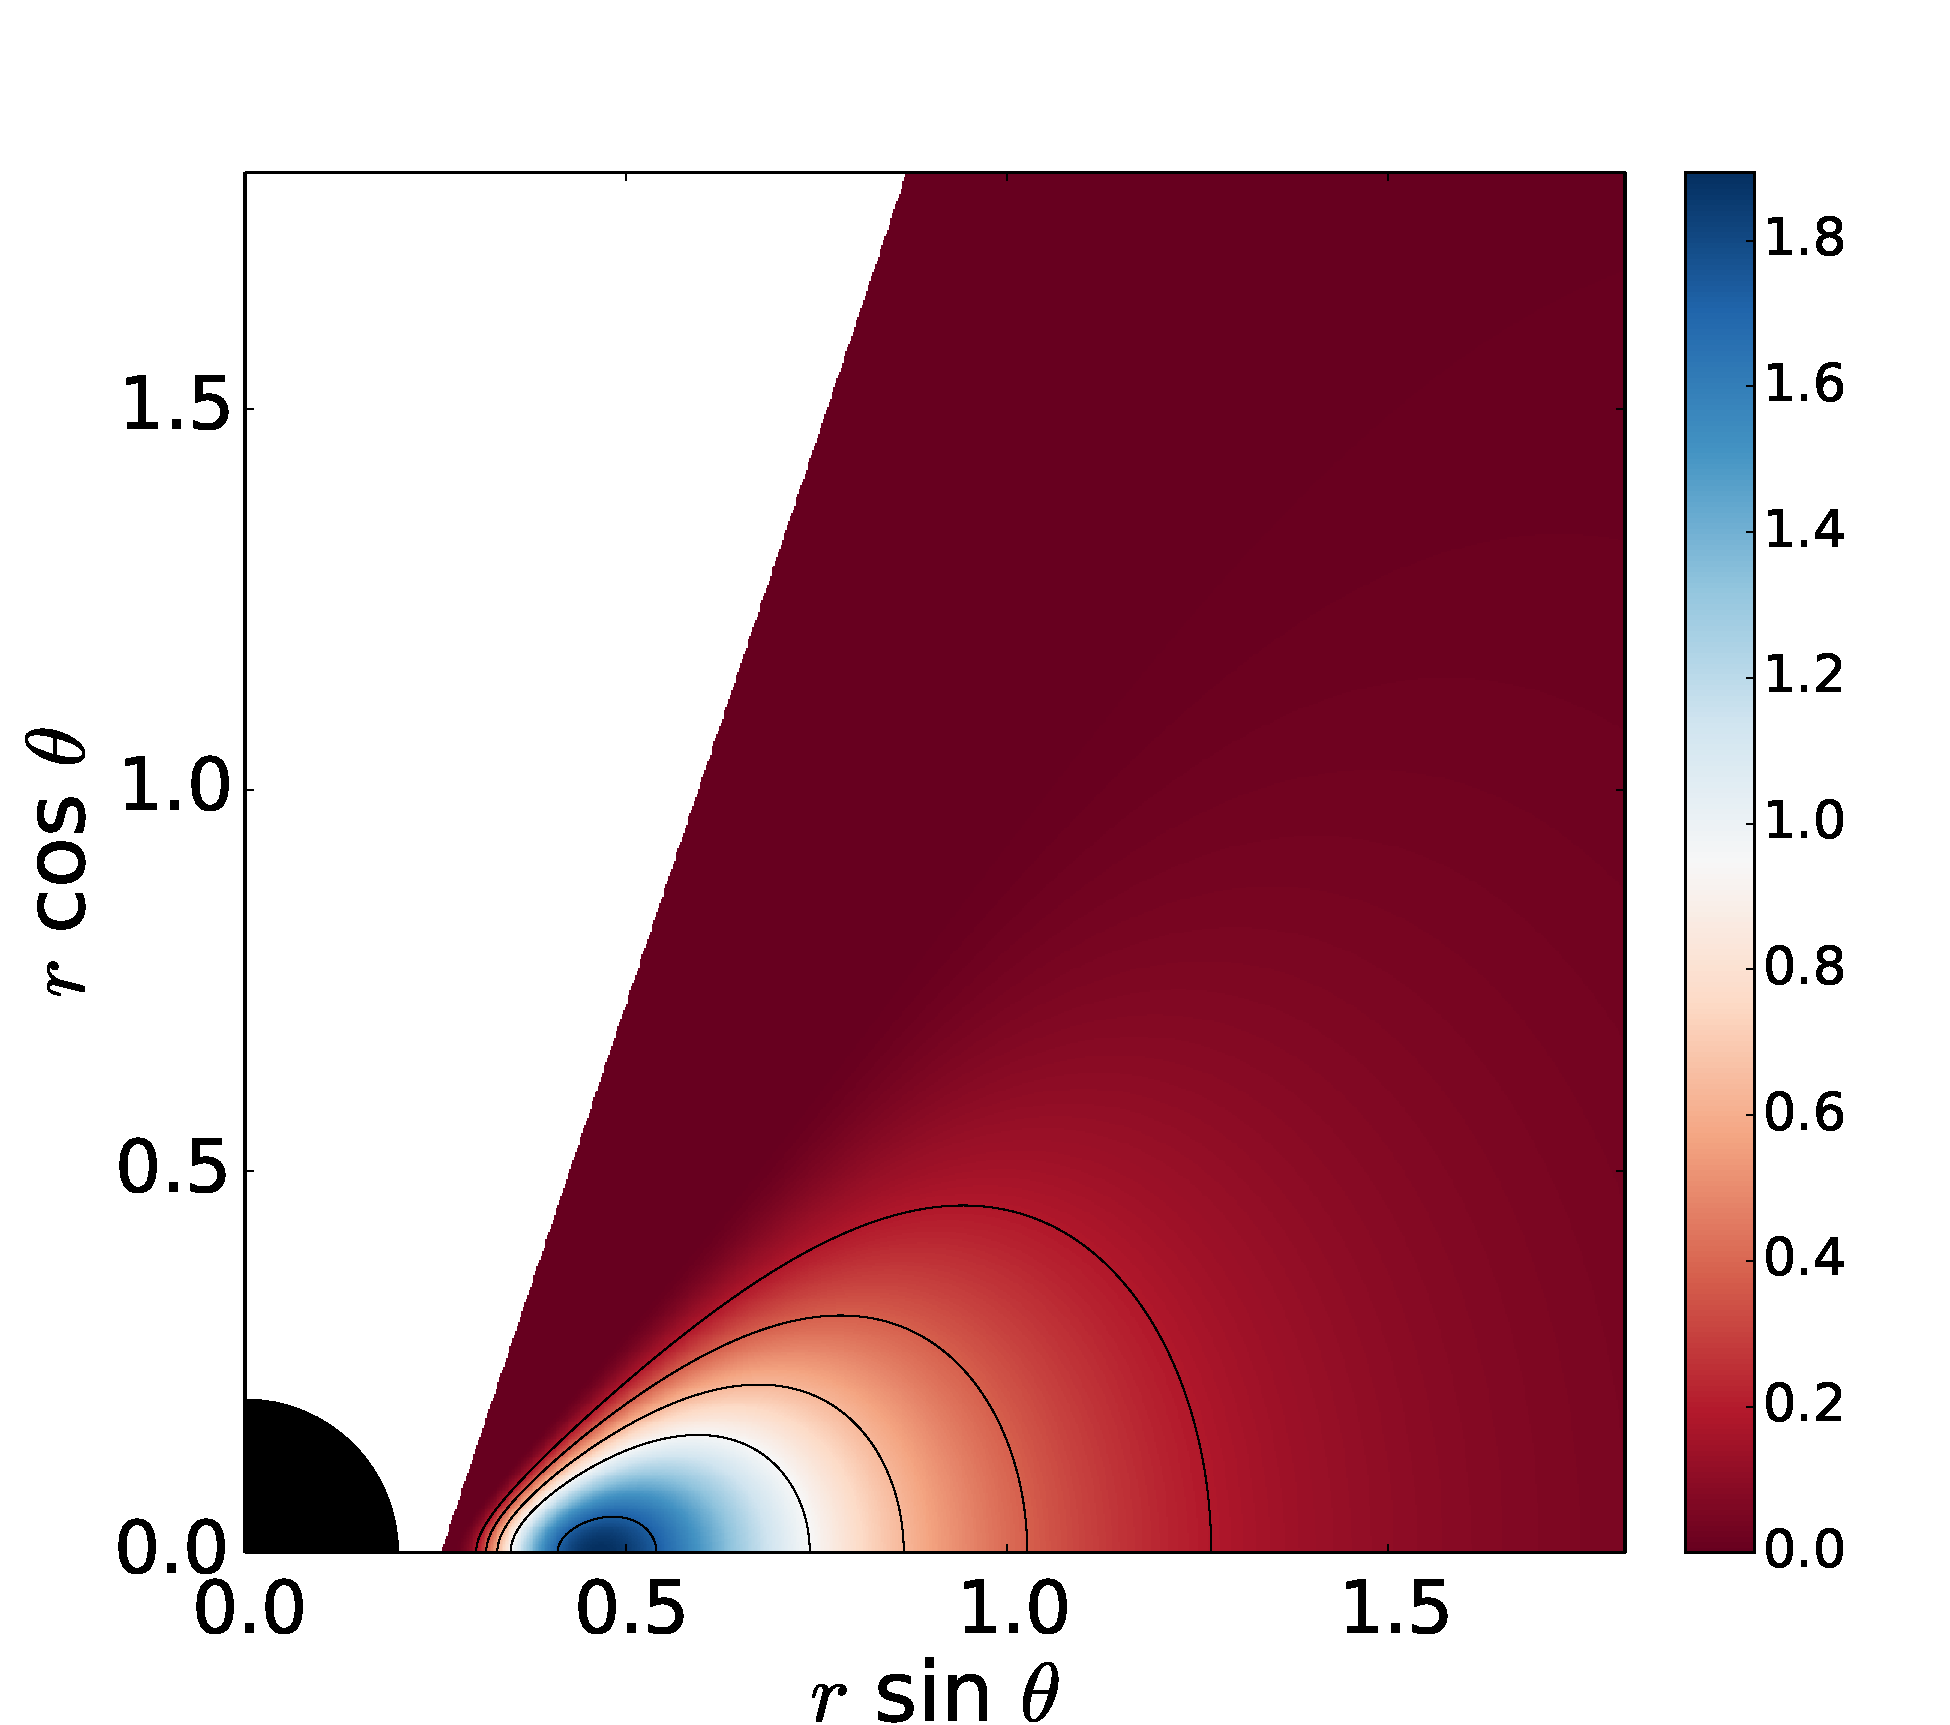
\includegraphics[scale=0.14]{figures/fig1_III__3.pdf}
\\
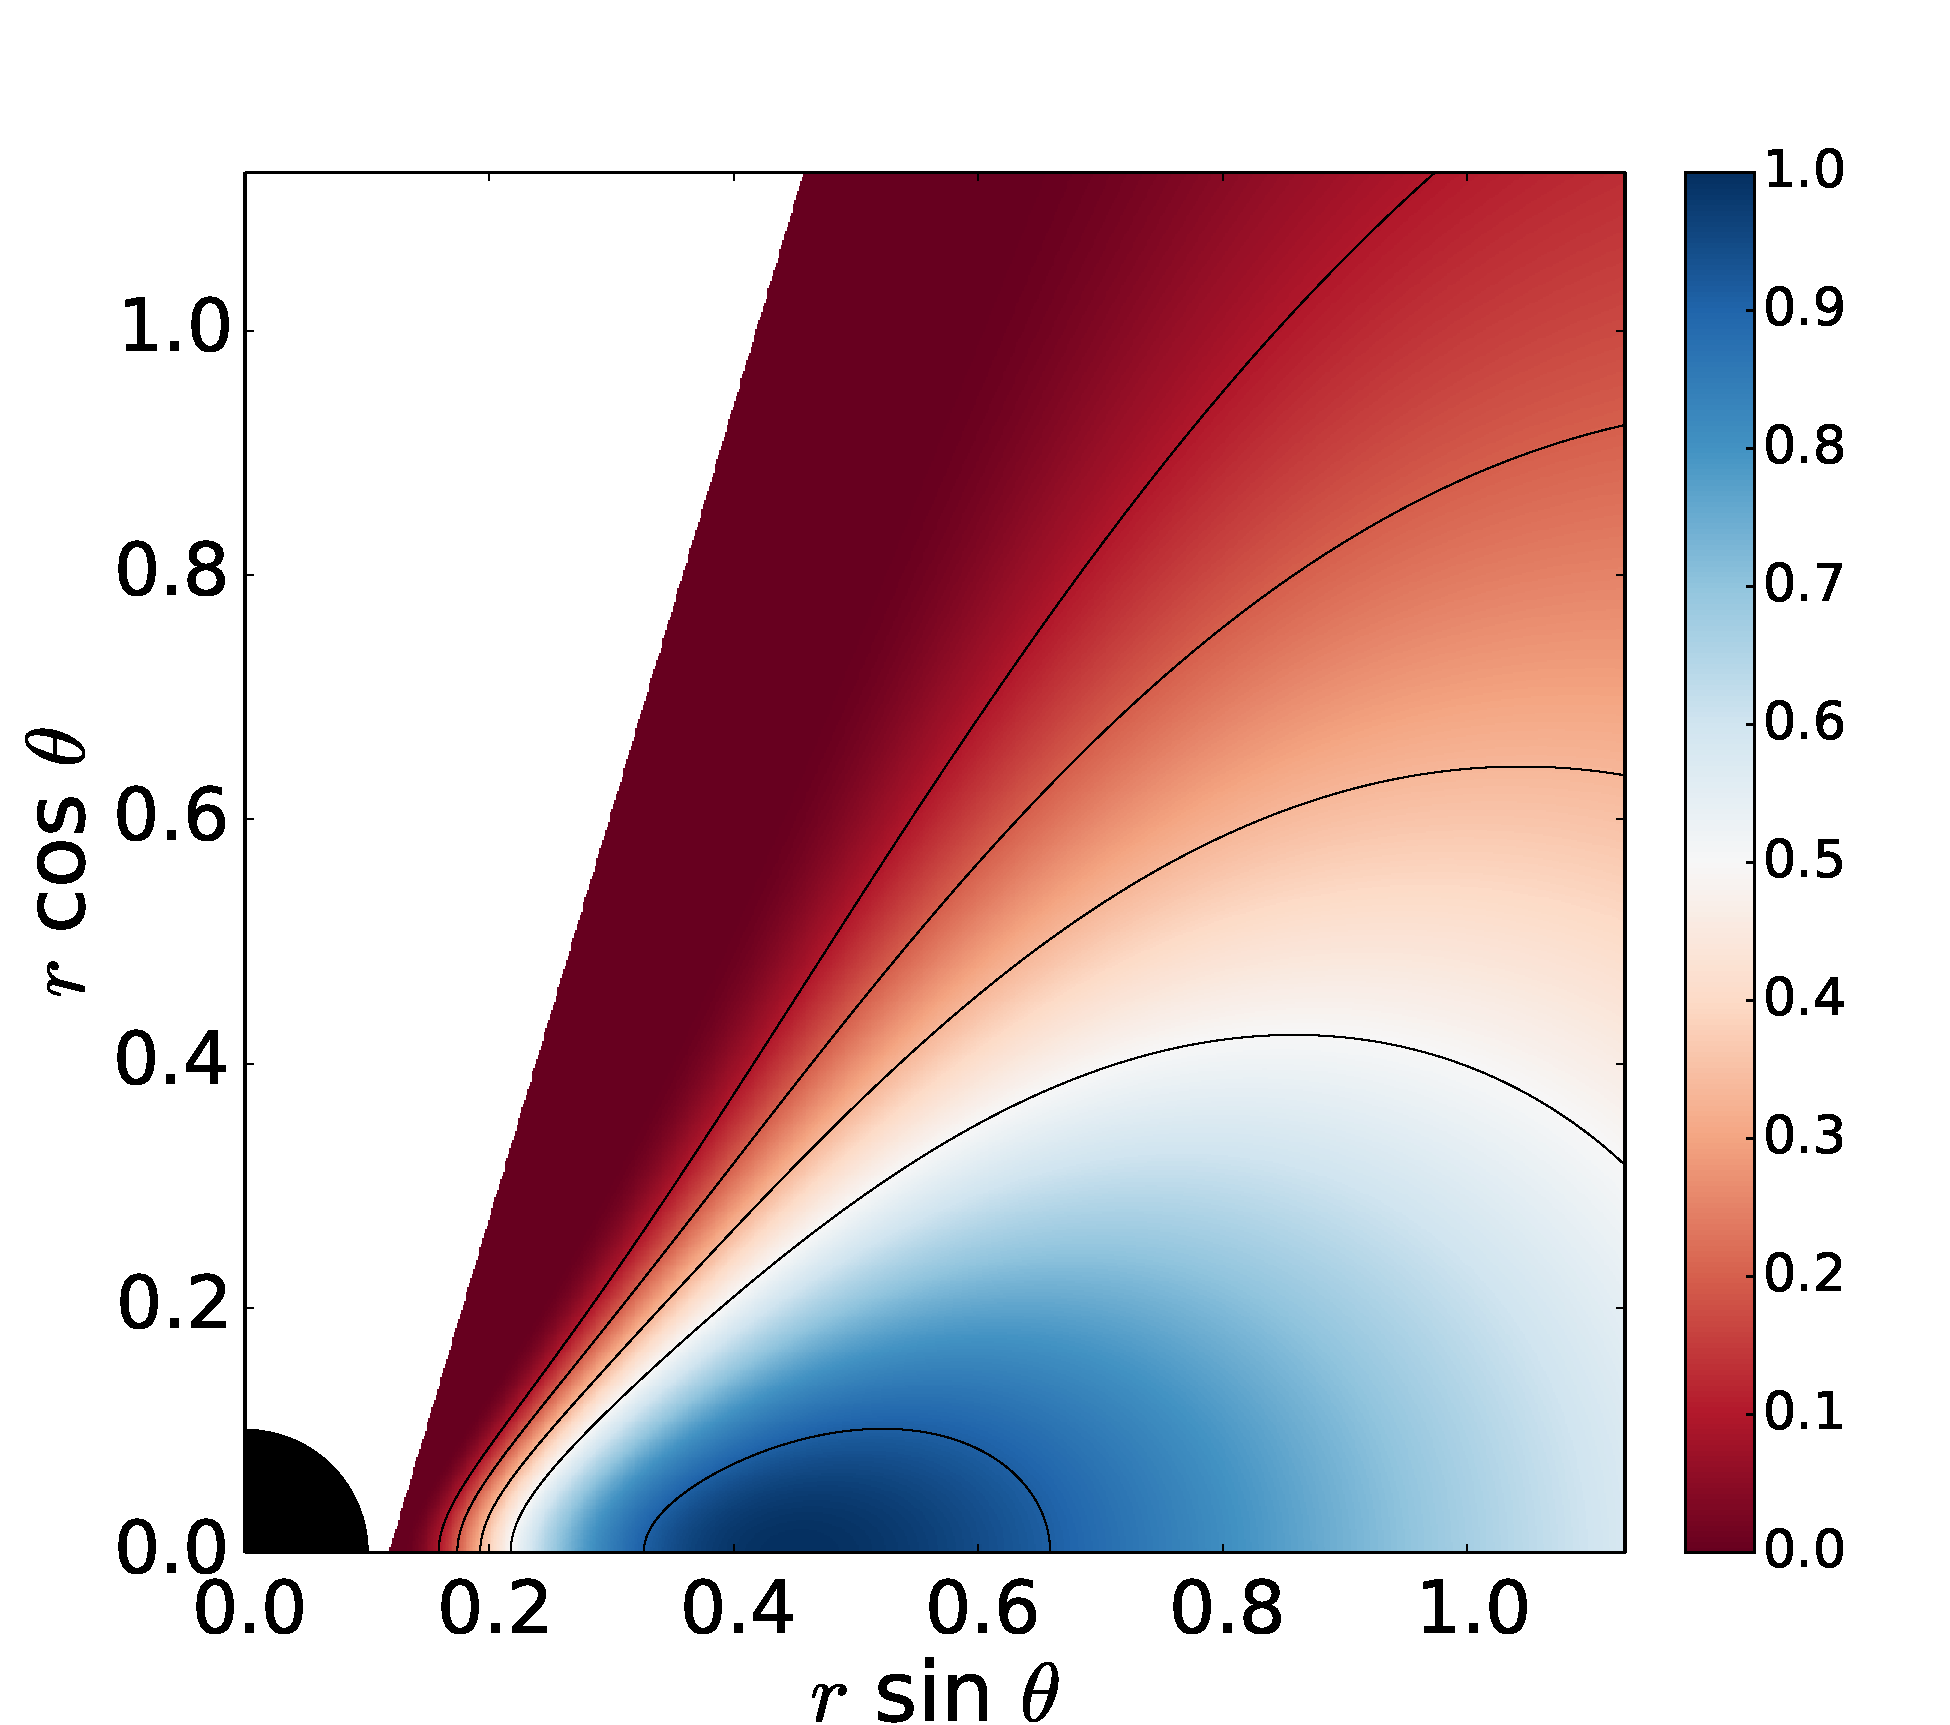
\includegraphics[scale=0.14]{figures/fig1_IV_3.pdf}
\hspace{-0.3cm}
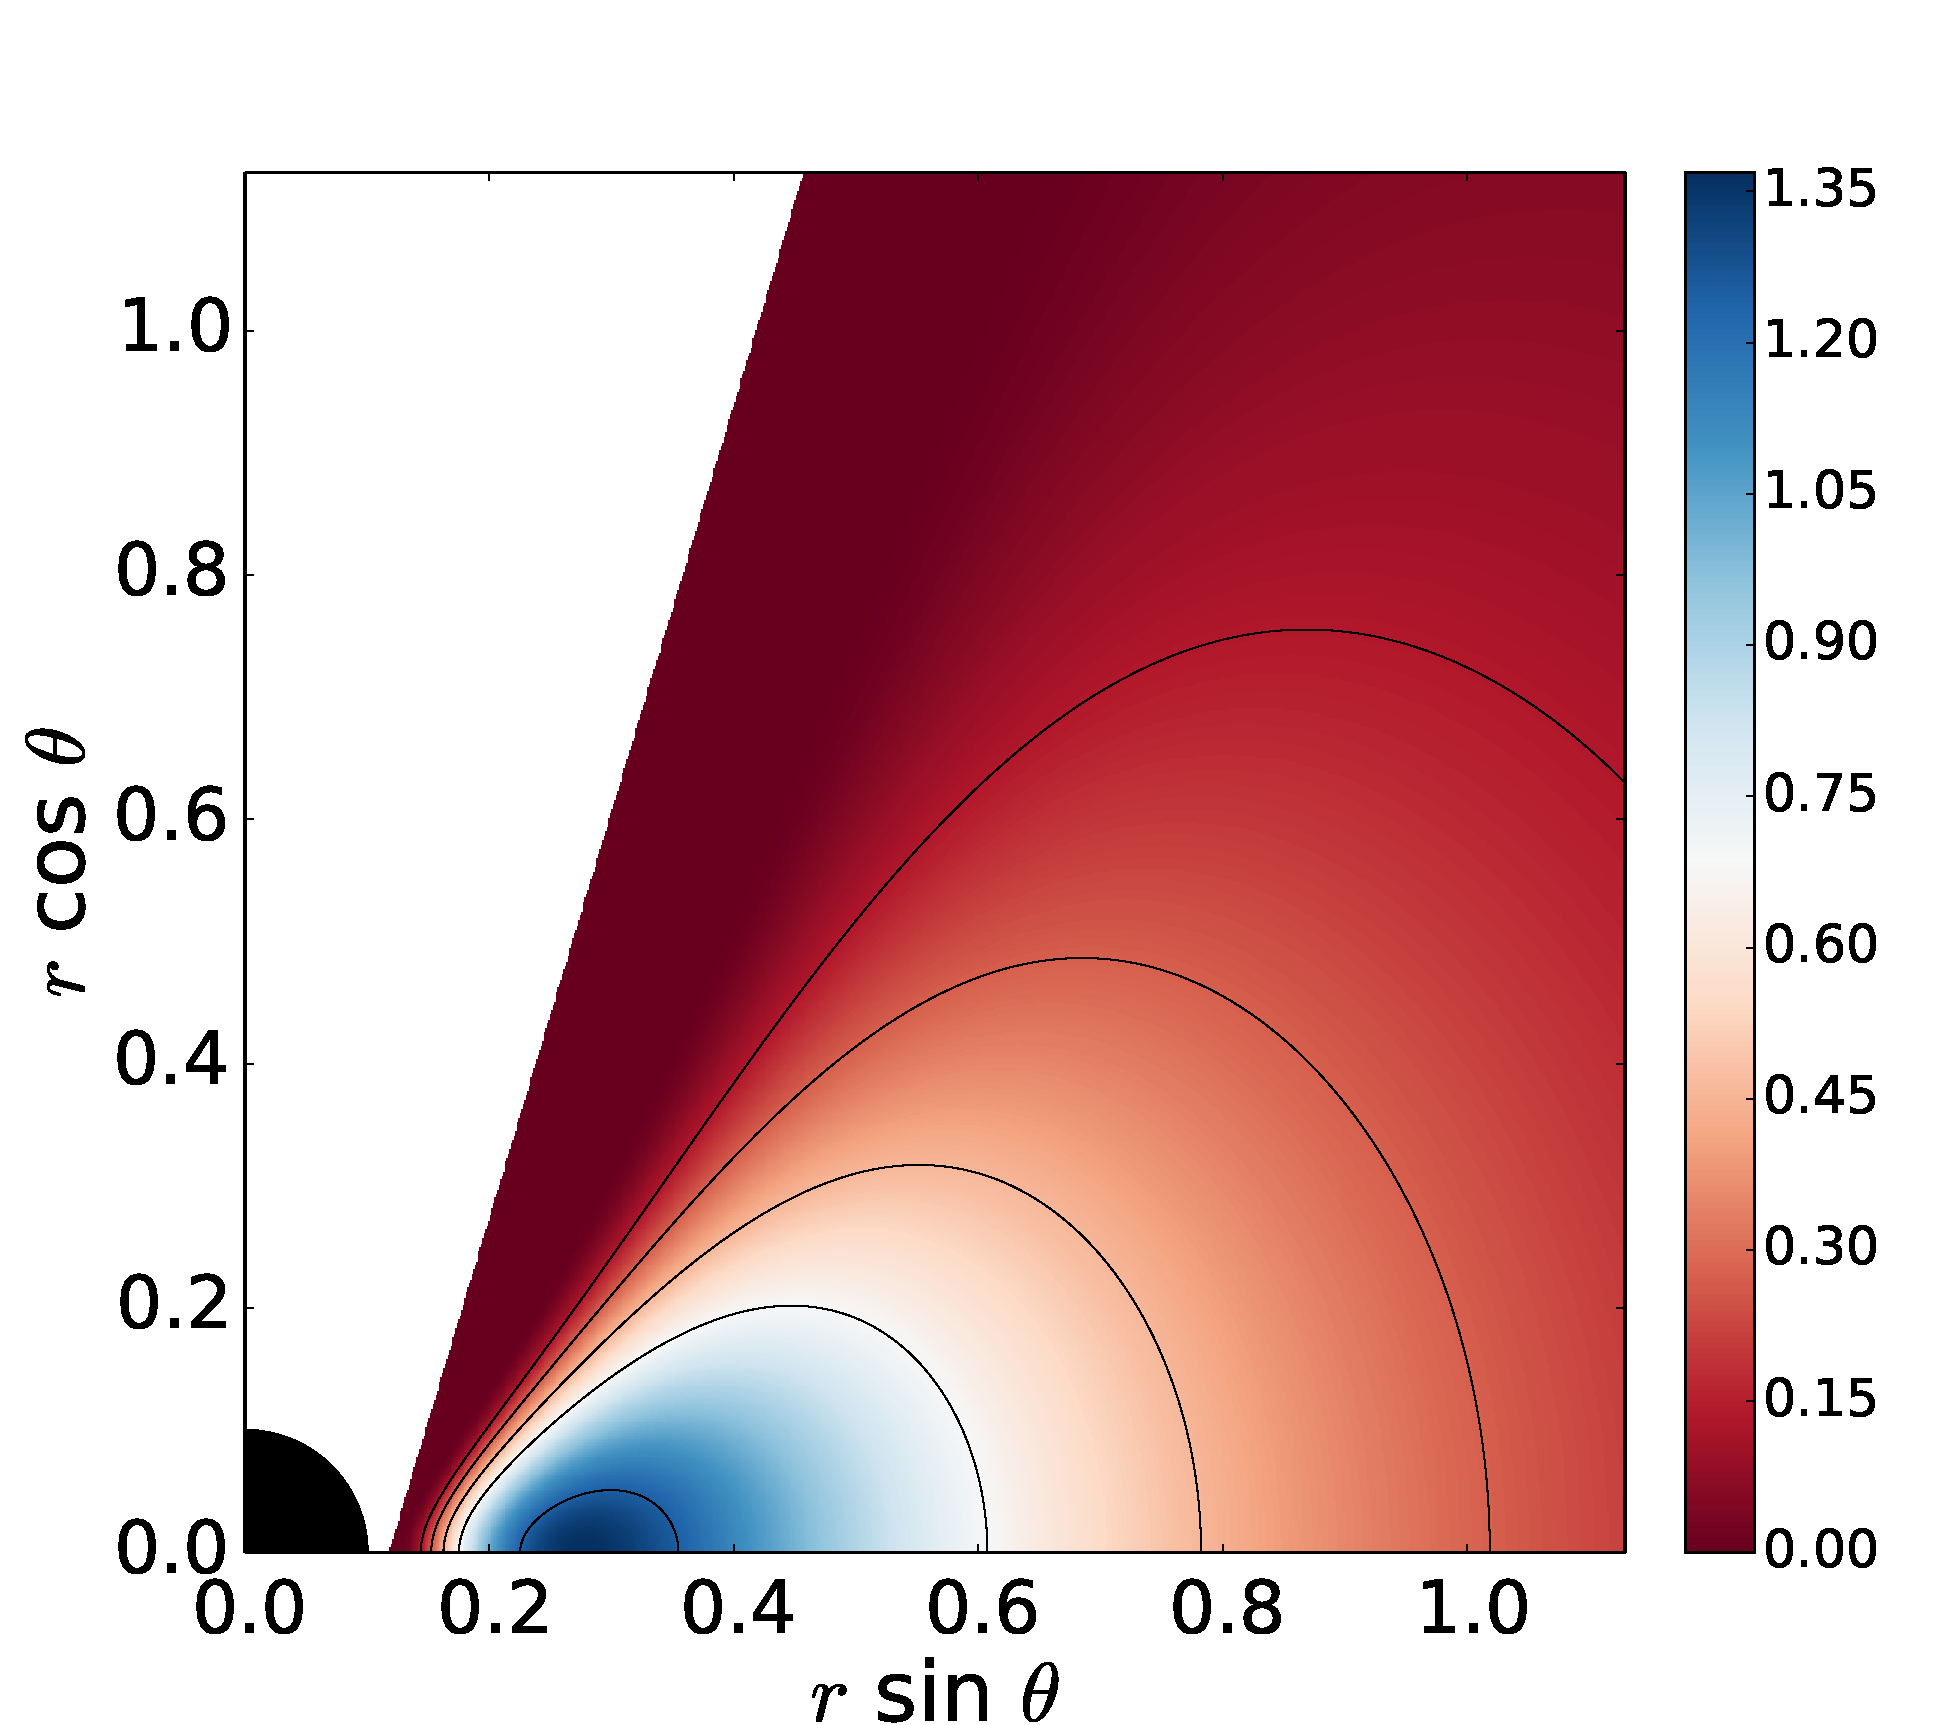
\includegraphics[scale=0.14]{figures/fig1_IV_0.pdf}
\hspace{-0.2cm}
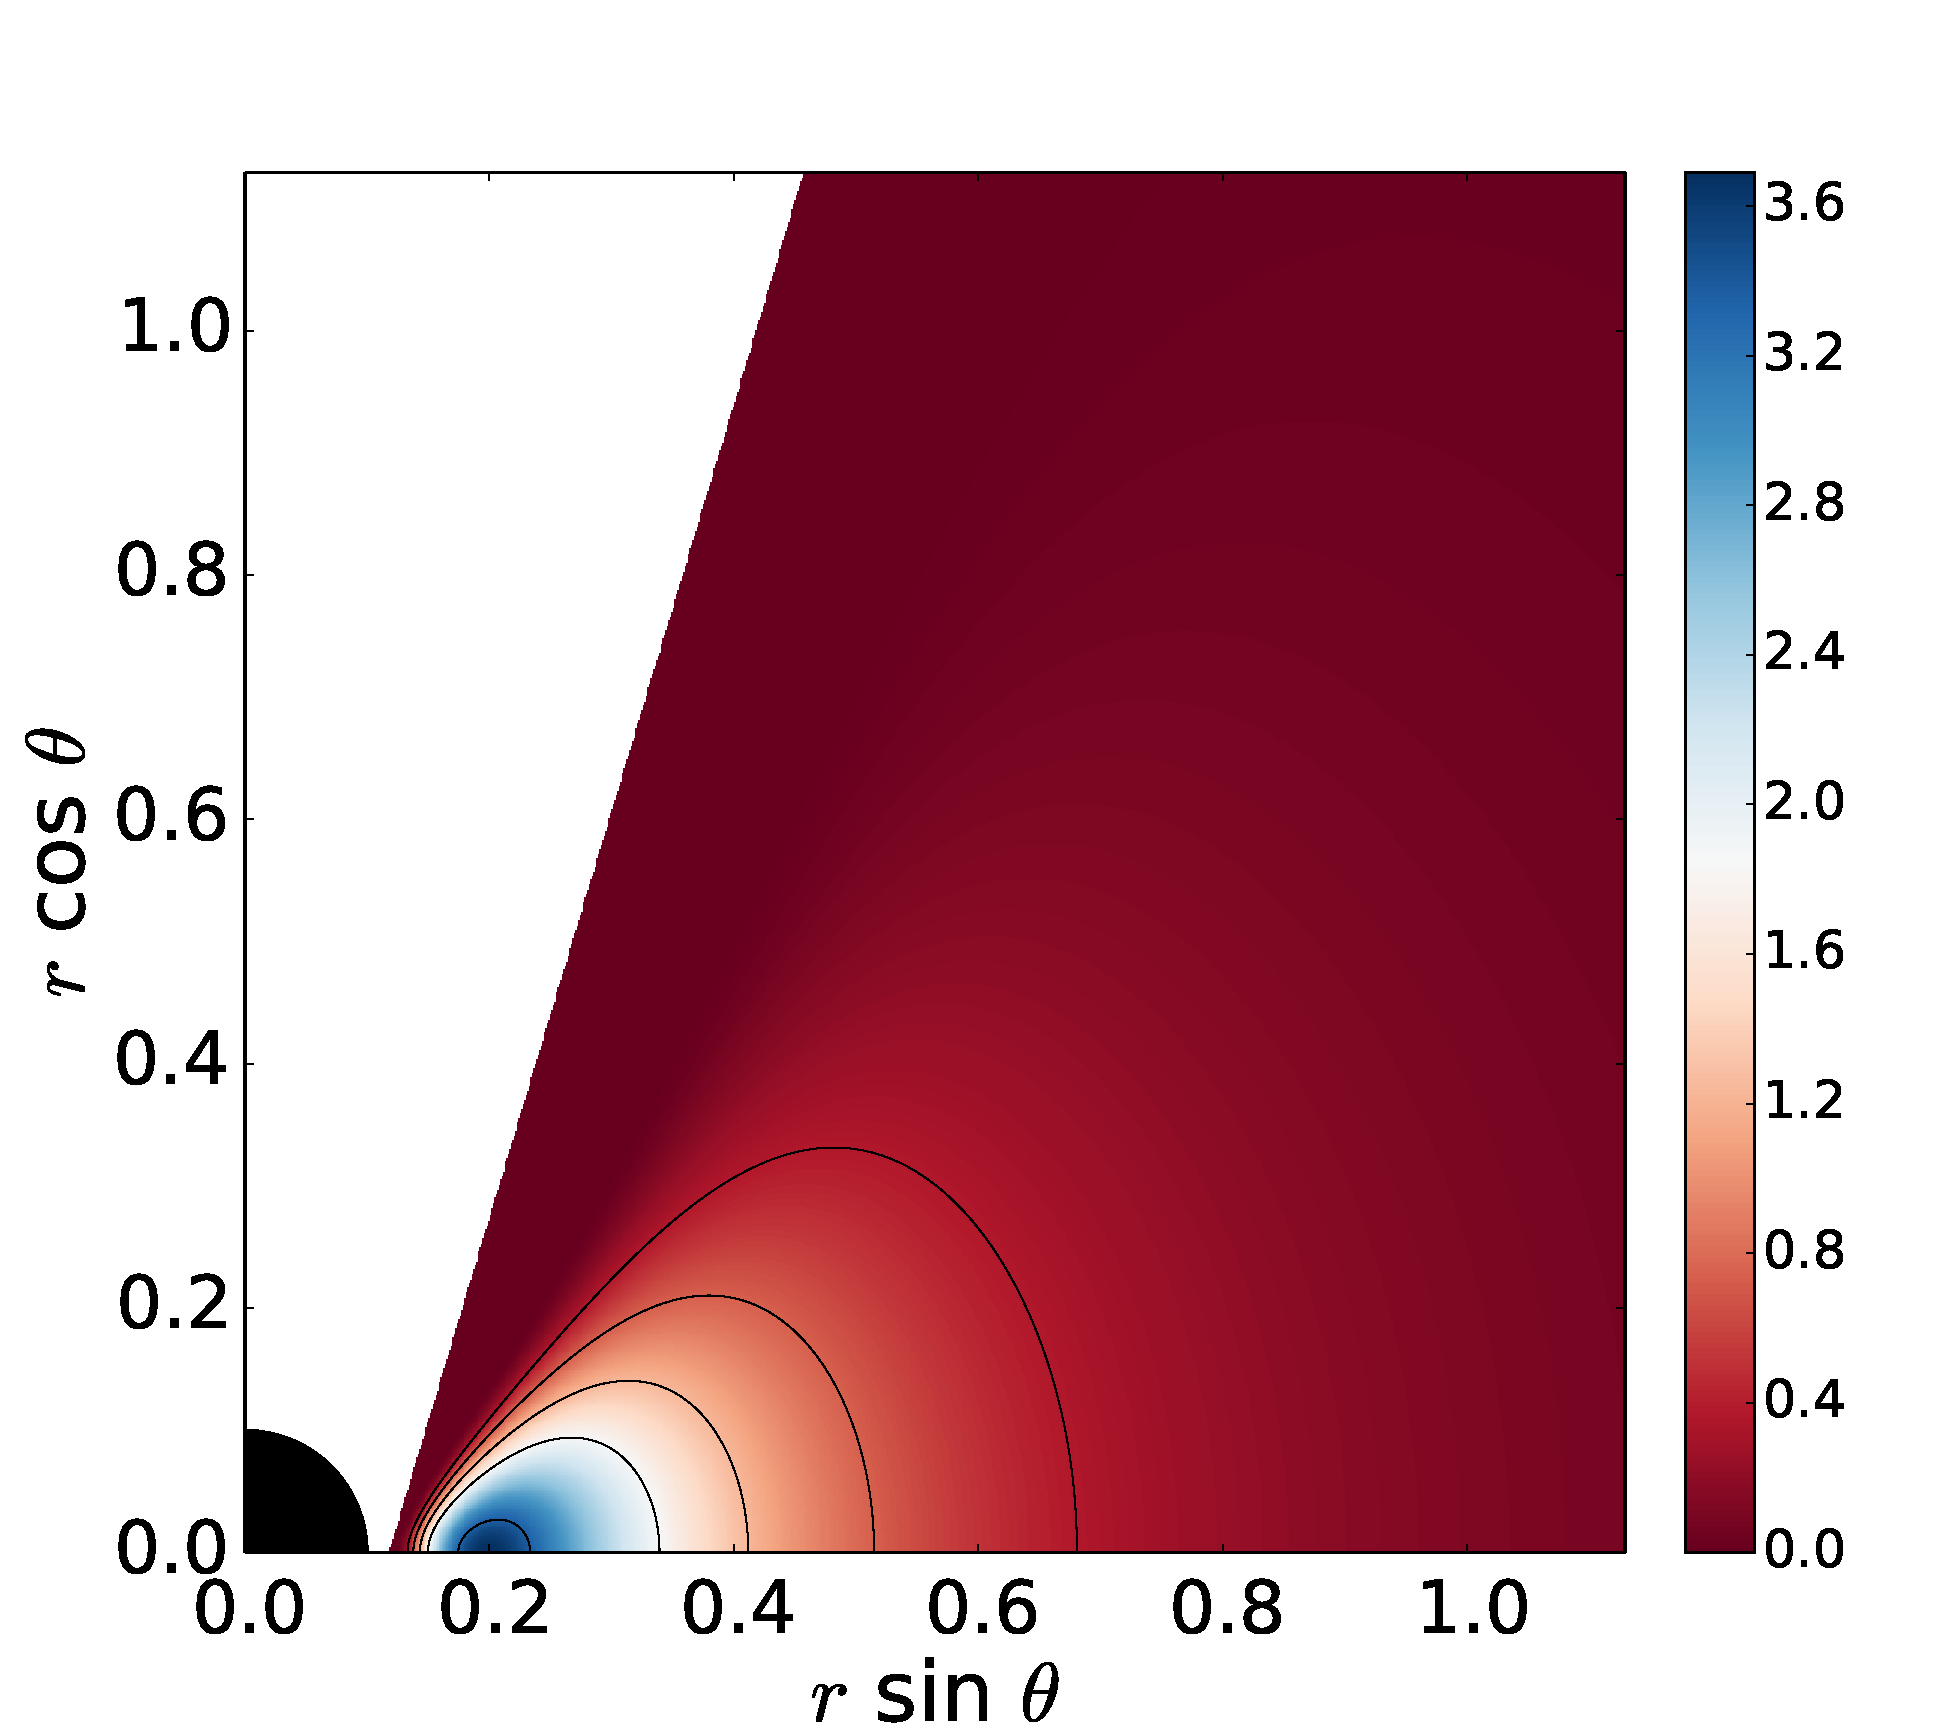
\includegraphics[scale=0.14]{figures/fig1_IV__3.pdf}
\\
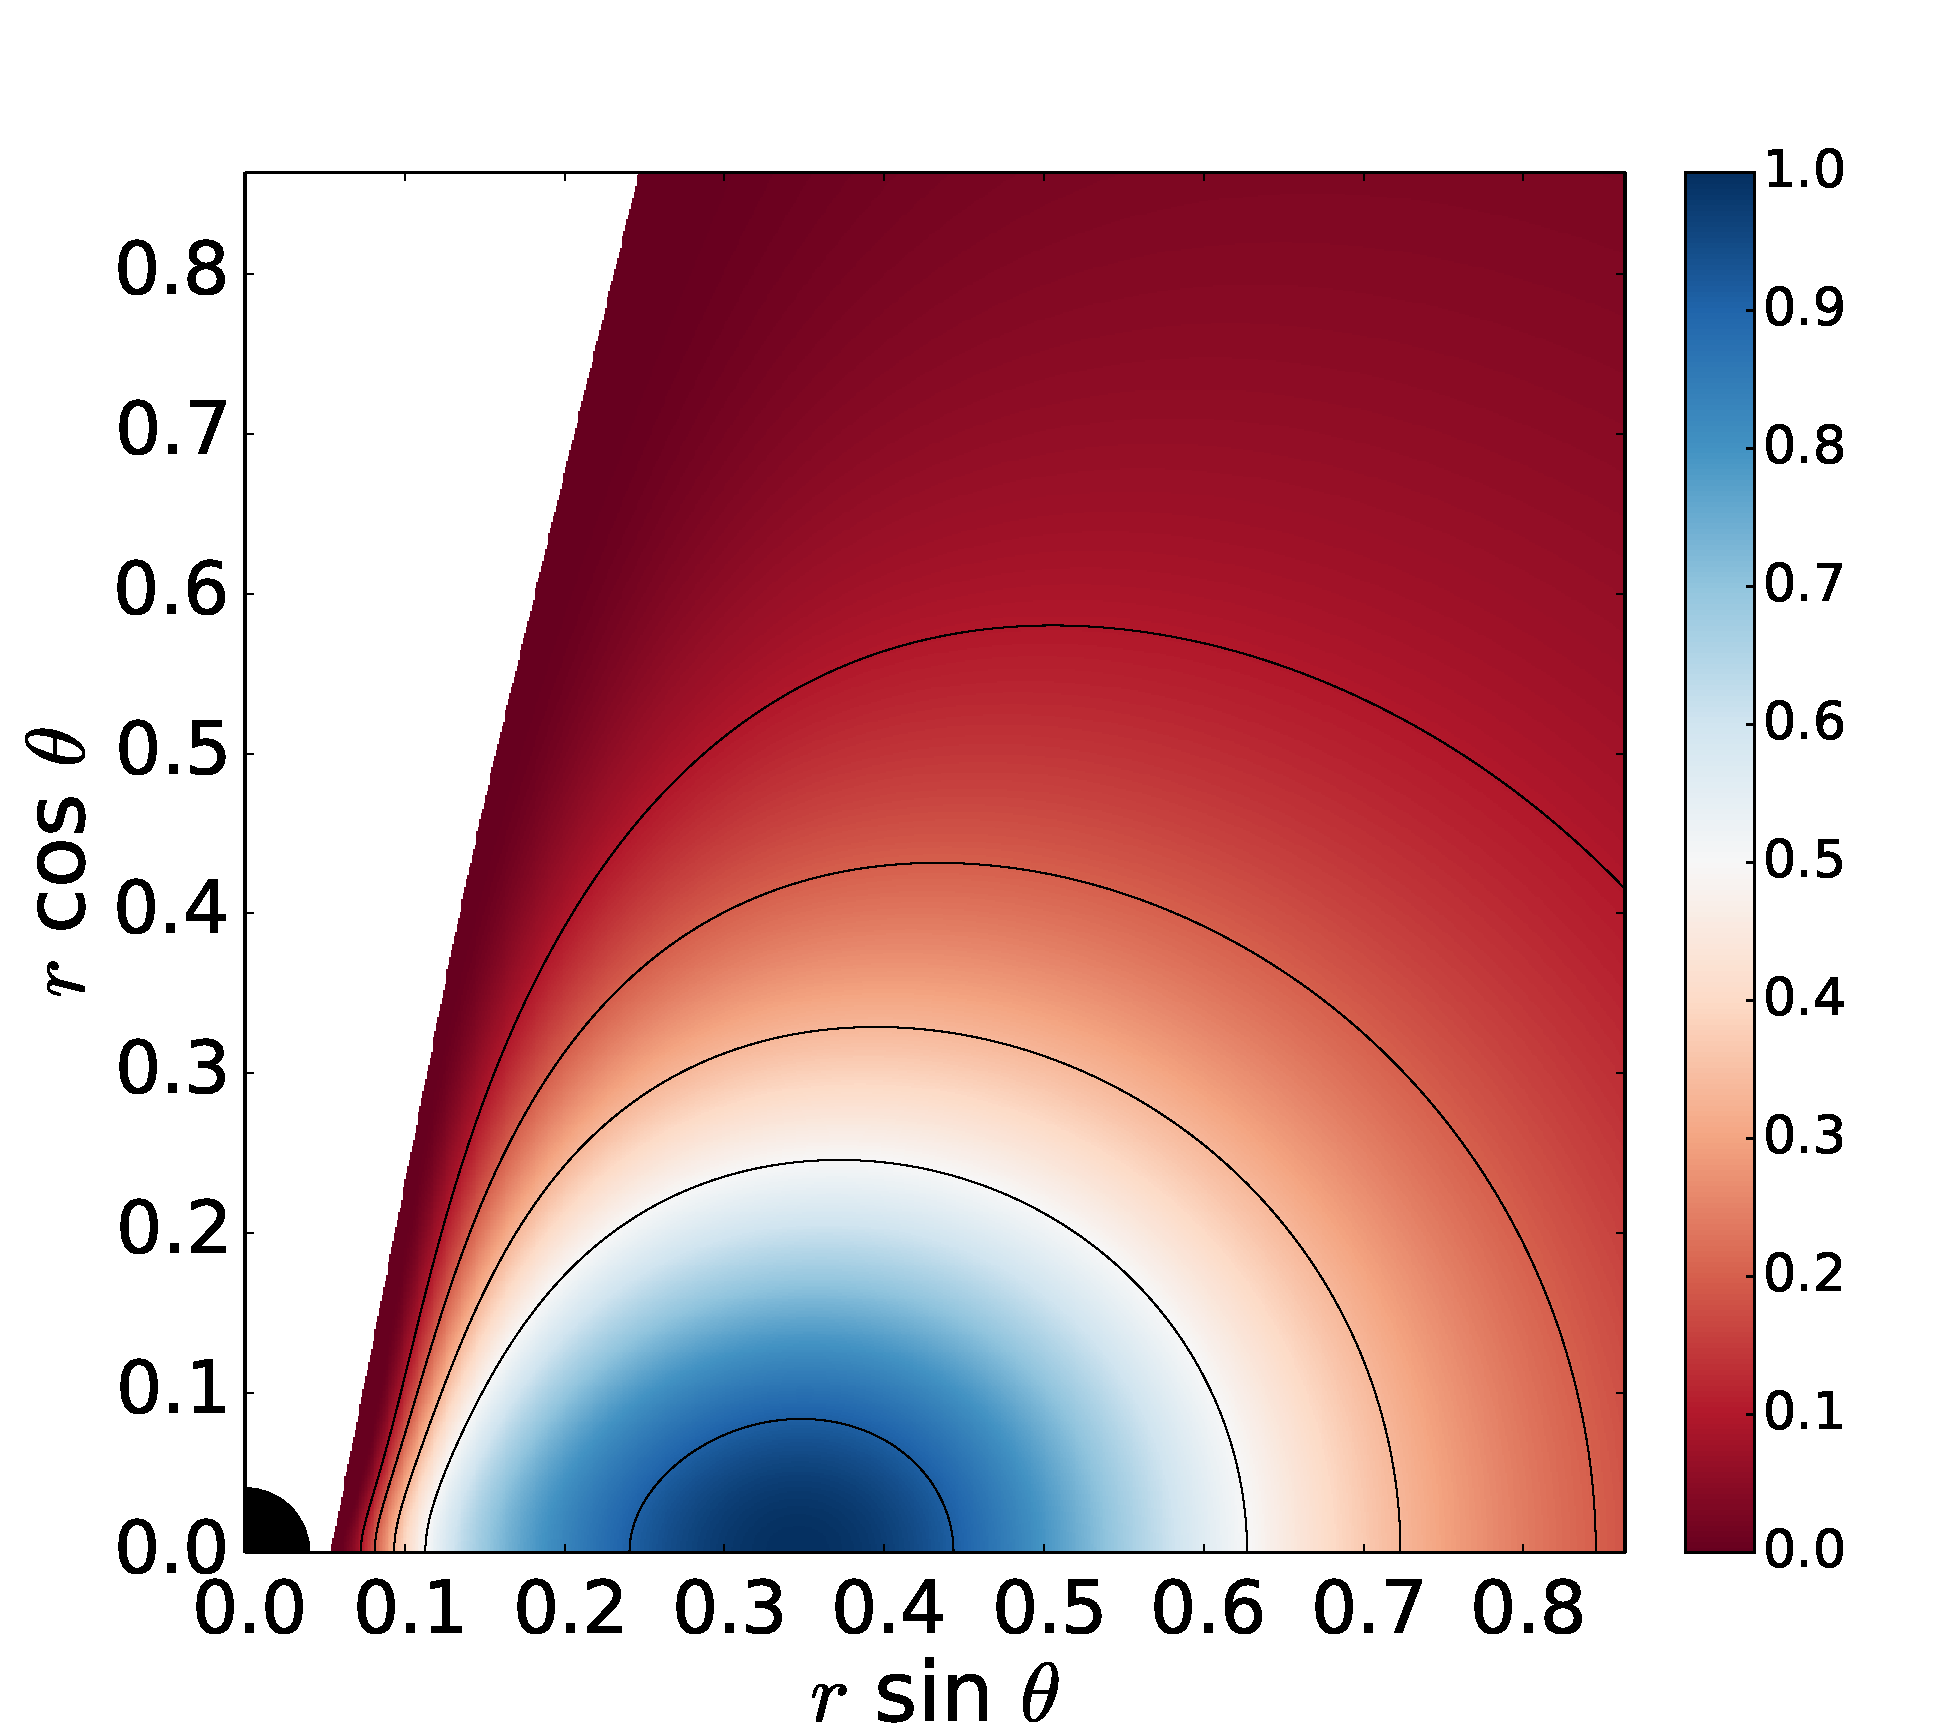
\includegraphics[scale=0.14]{figures/fig1_V_3.pdf}
\hspace{-0.3cm}
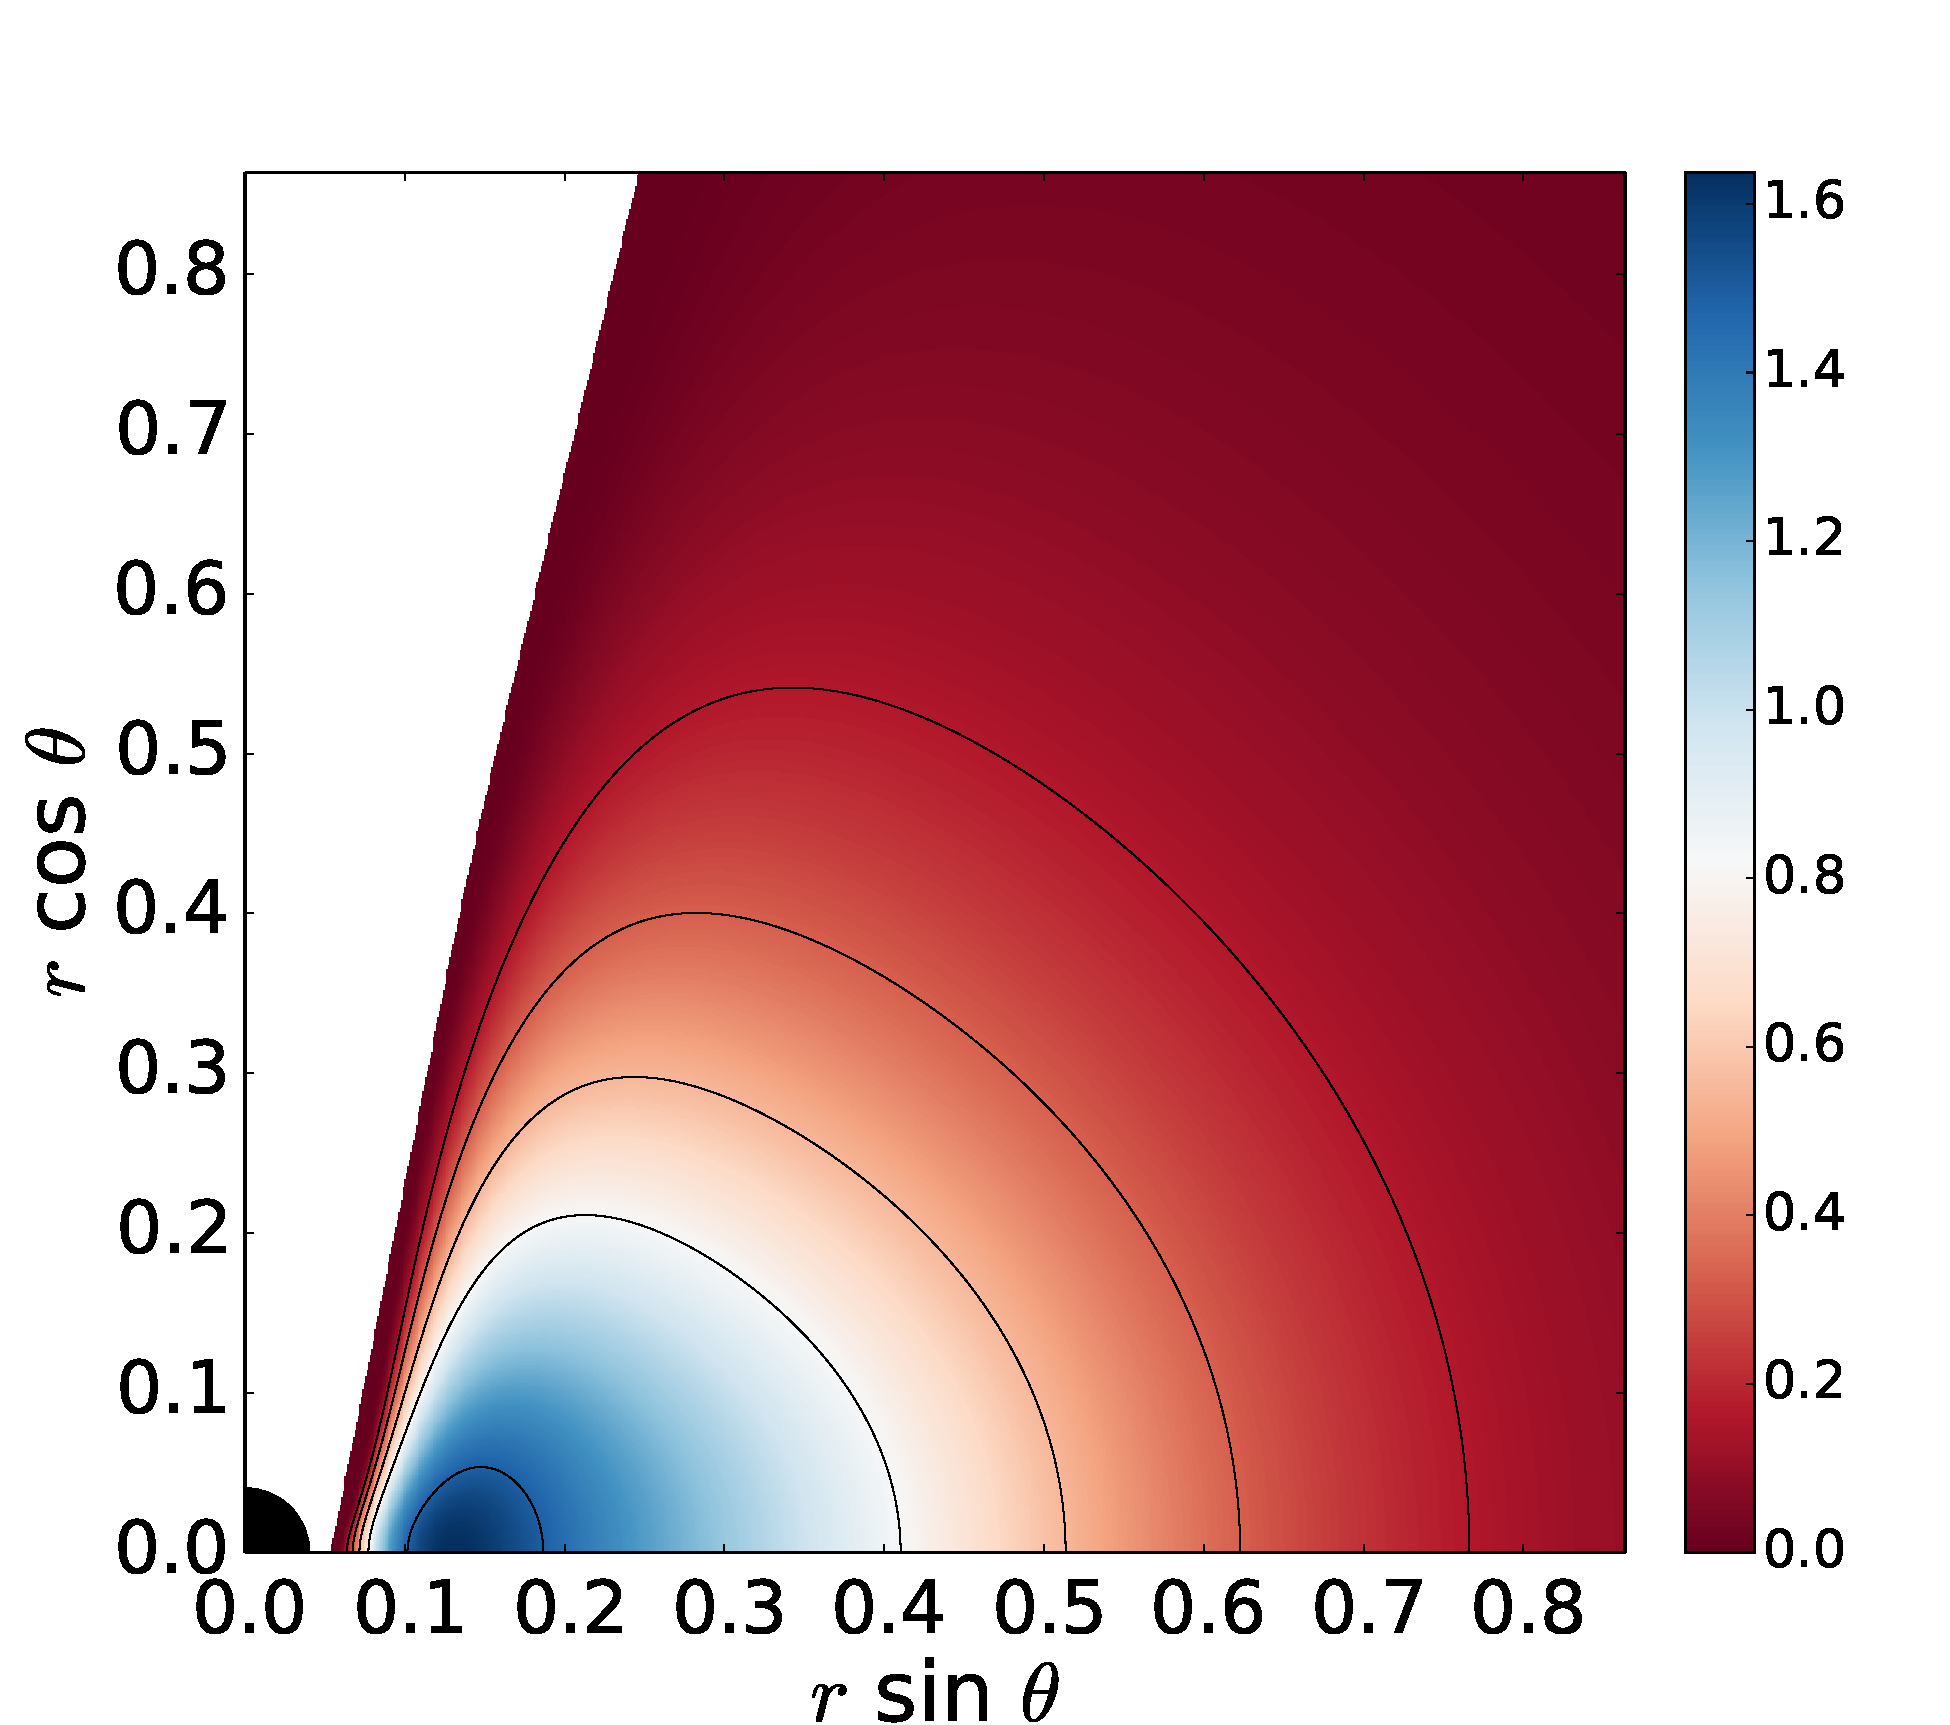
\includegraphics[scale=0.14]{figures/fig1_V_0.pdf}
\hspace{-0.2cm}
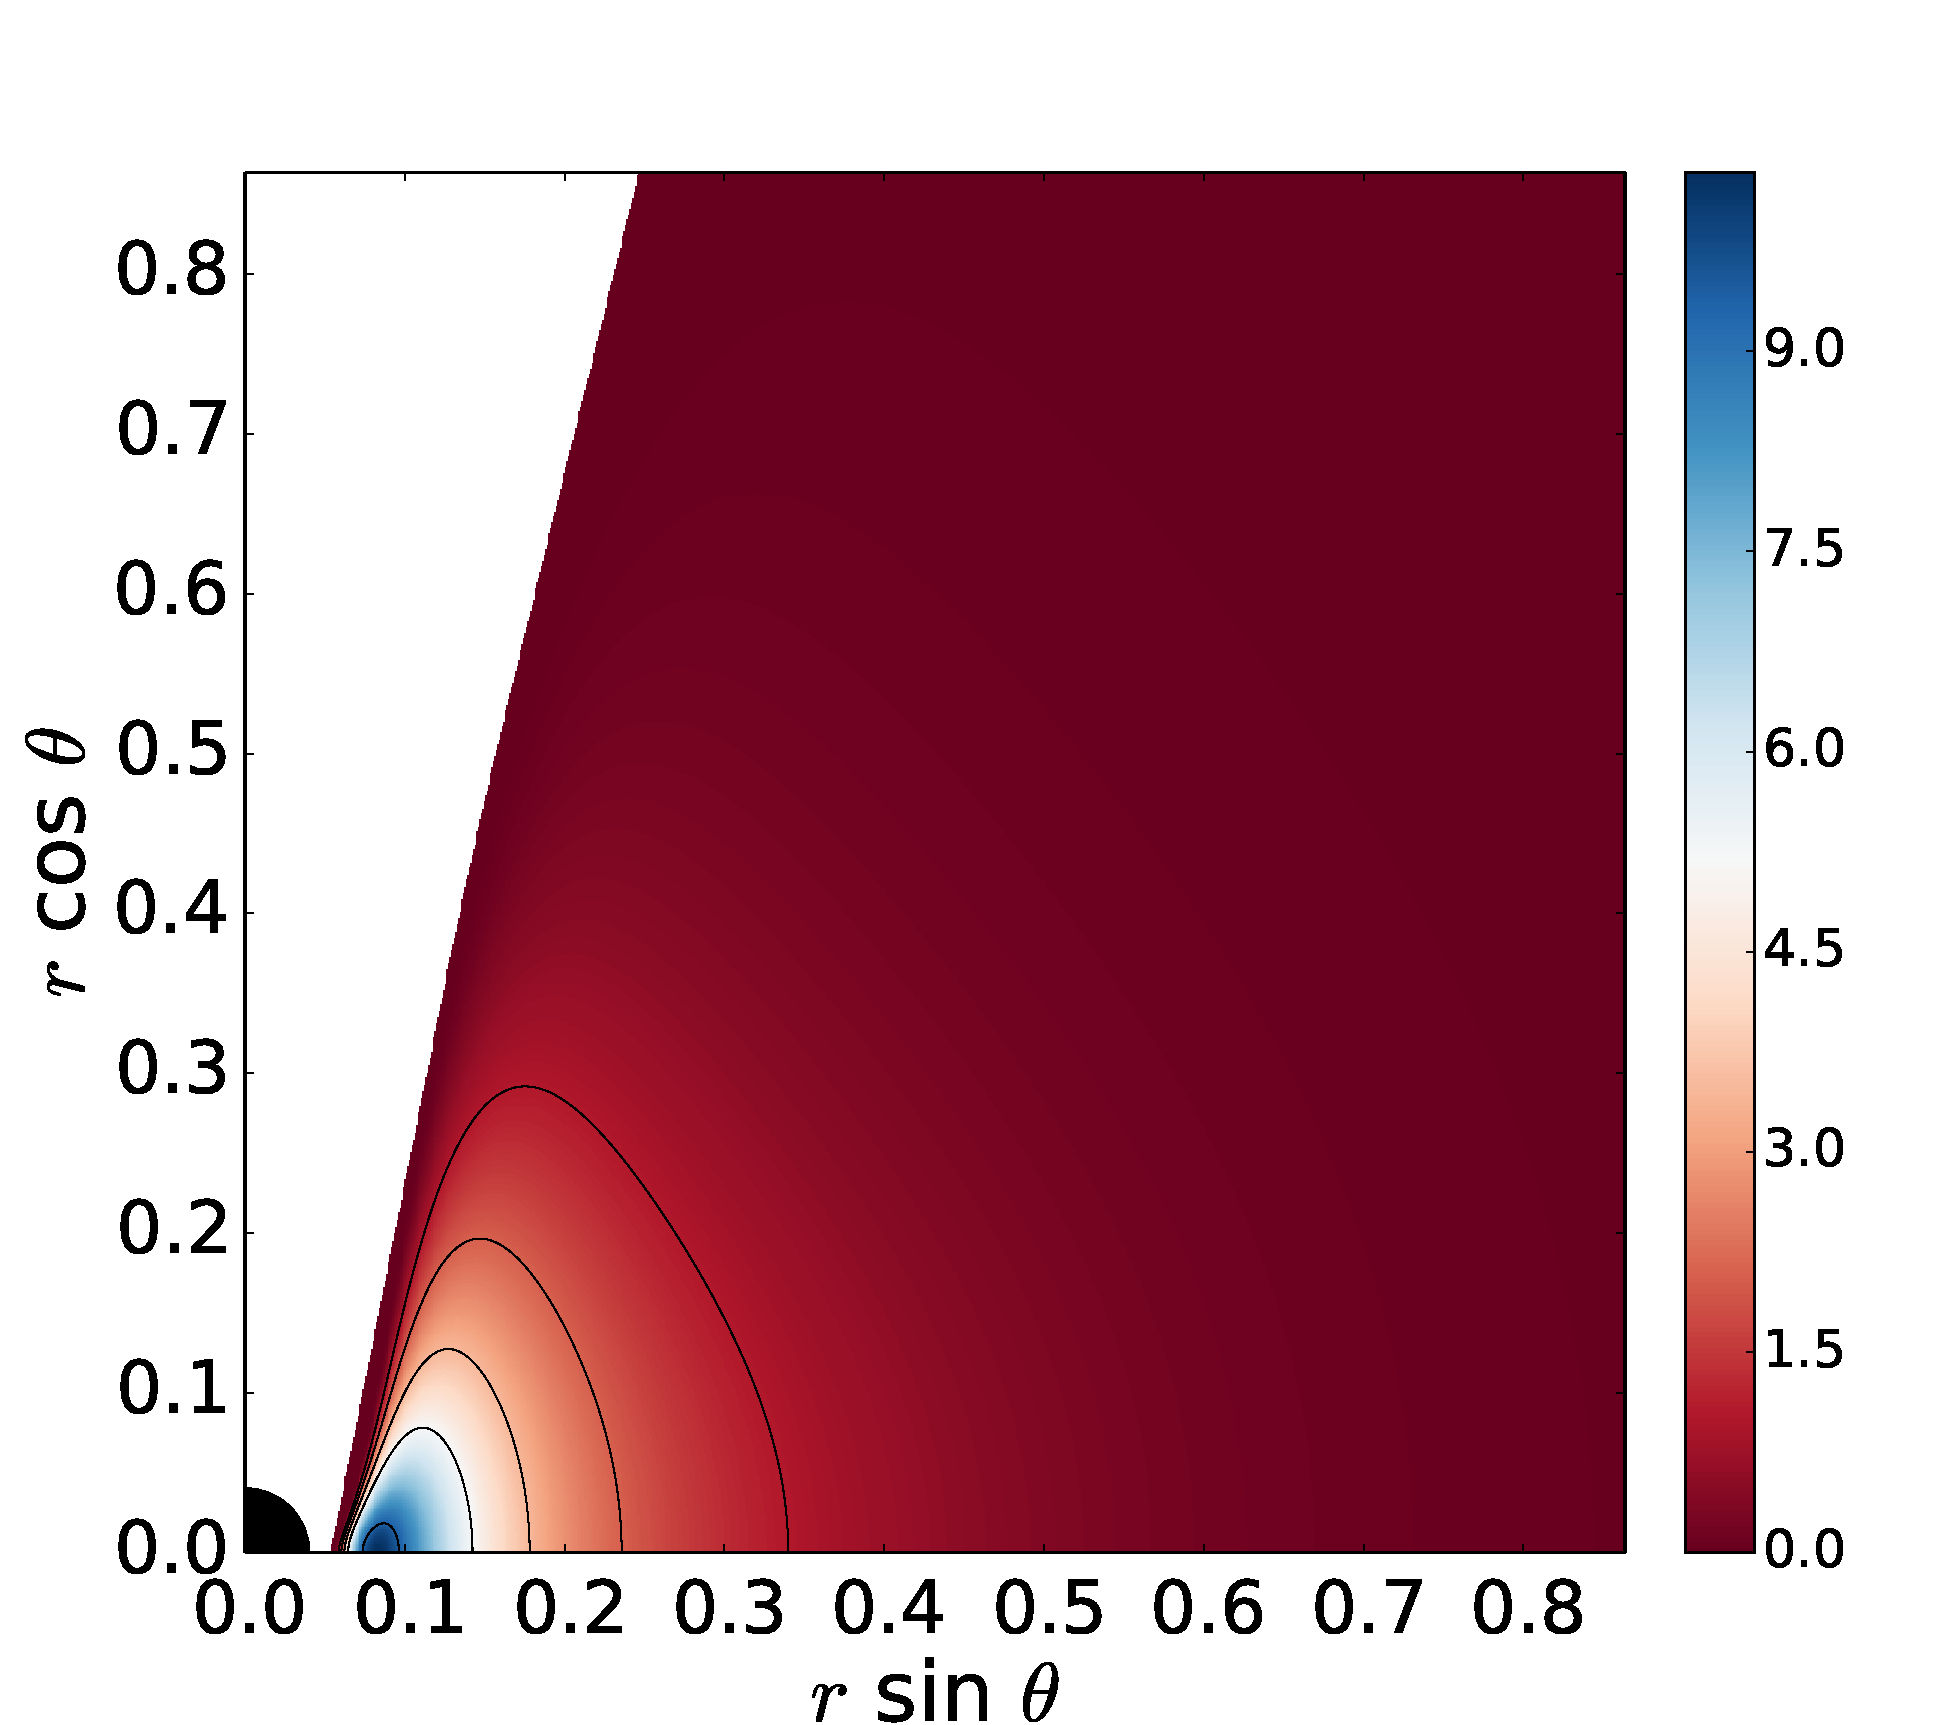
\includegraphics[scale=0.14]{figures/fig1_V__3.pdf}
\caption{Rest-mass density distribution. From top to bottom the rows correspond to the different models for the KBHsSH (I, II and III). From left to right the columns correspond to different values of the magnetization parameter, namely non-magnetized ($\beta_{\mathrm{m}_{\mathrm{c}}} = 10^{3}$), mildly magnetized ($\beta_{\mathrm{m}_{\mathrm{c}}} = 1$) and strongly magnetized ($\beta_{\mathrm{m}_{\mathrm{c}}} = 10^{-3}$)}
\label{models}
\end{figure*}

\begin{figure*}
\centering
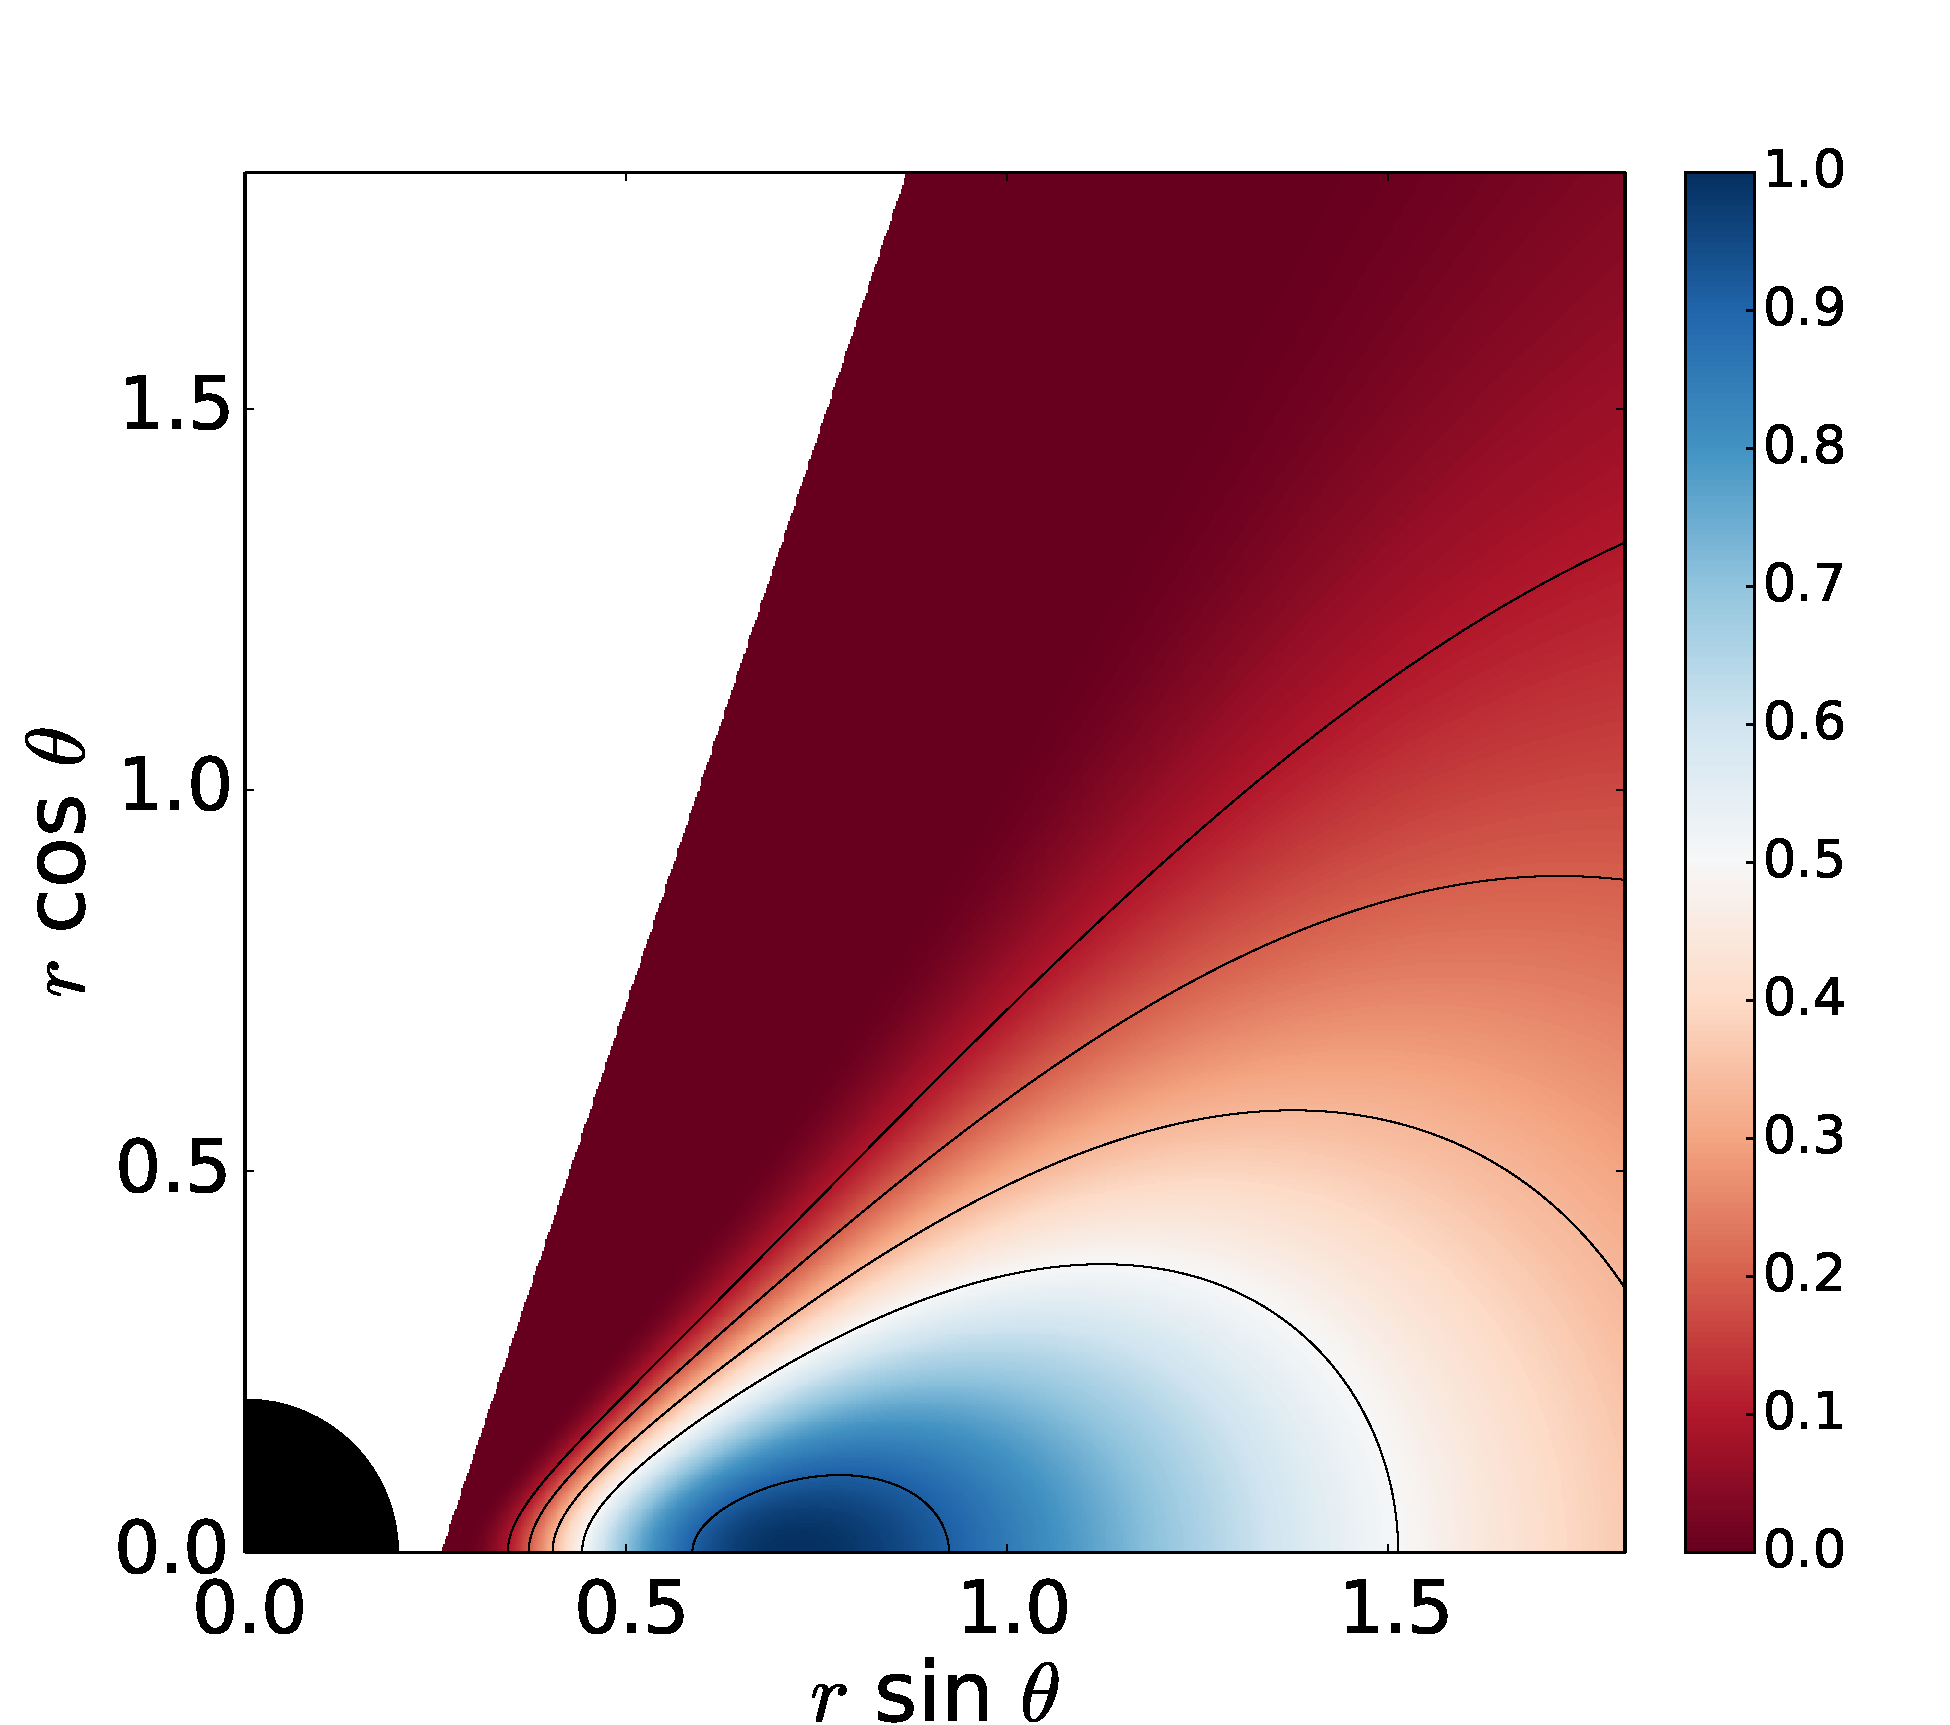
\includegraphics[scale=0.2]{figures/fig2_III_HBH_3.pdf}
\hspace{-0.3cm}
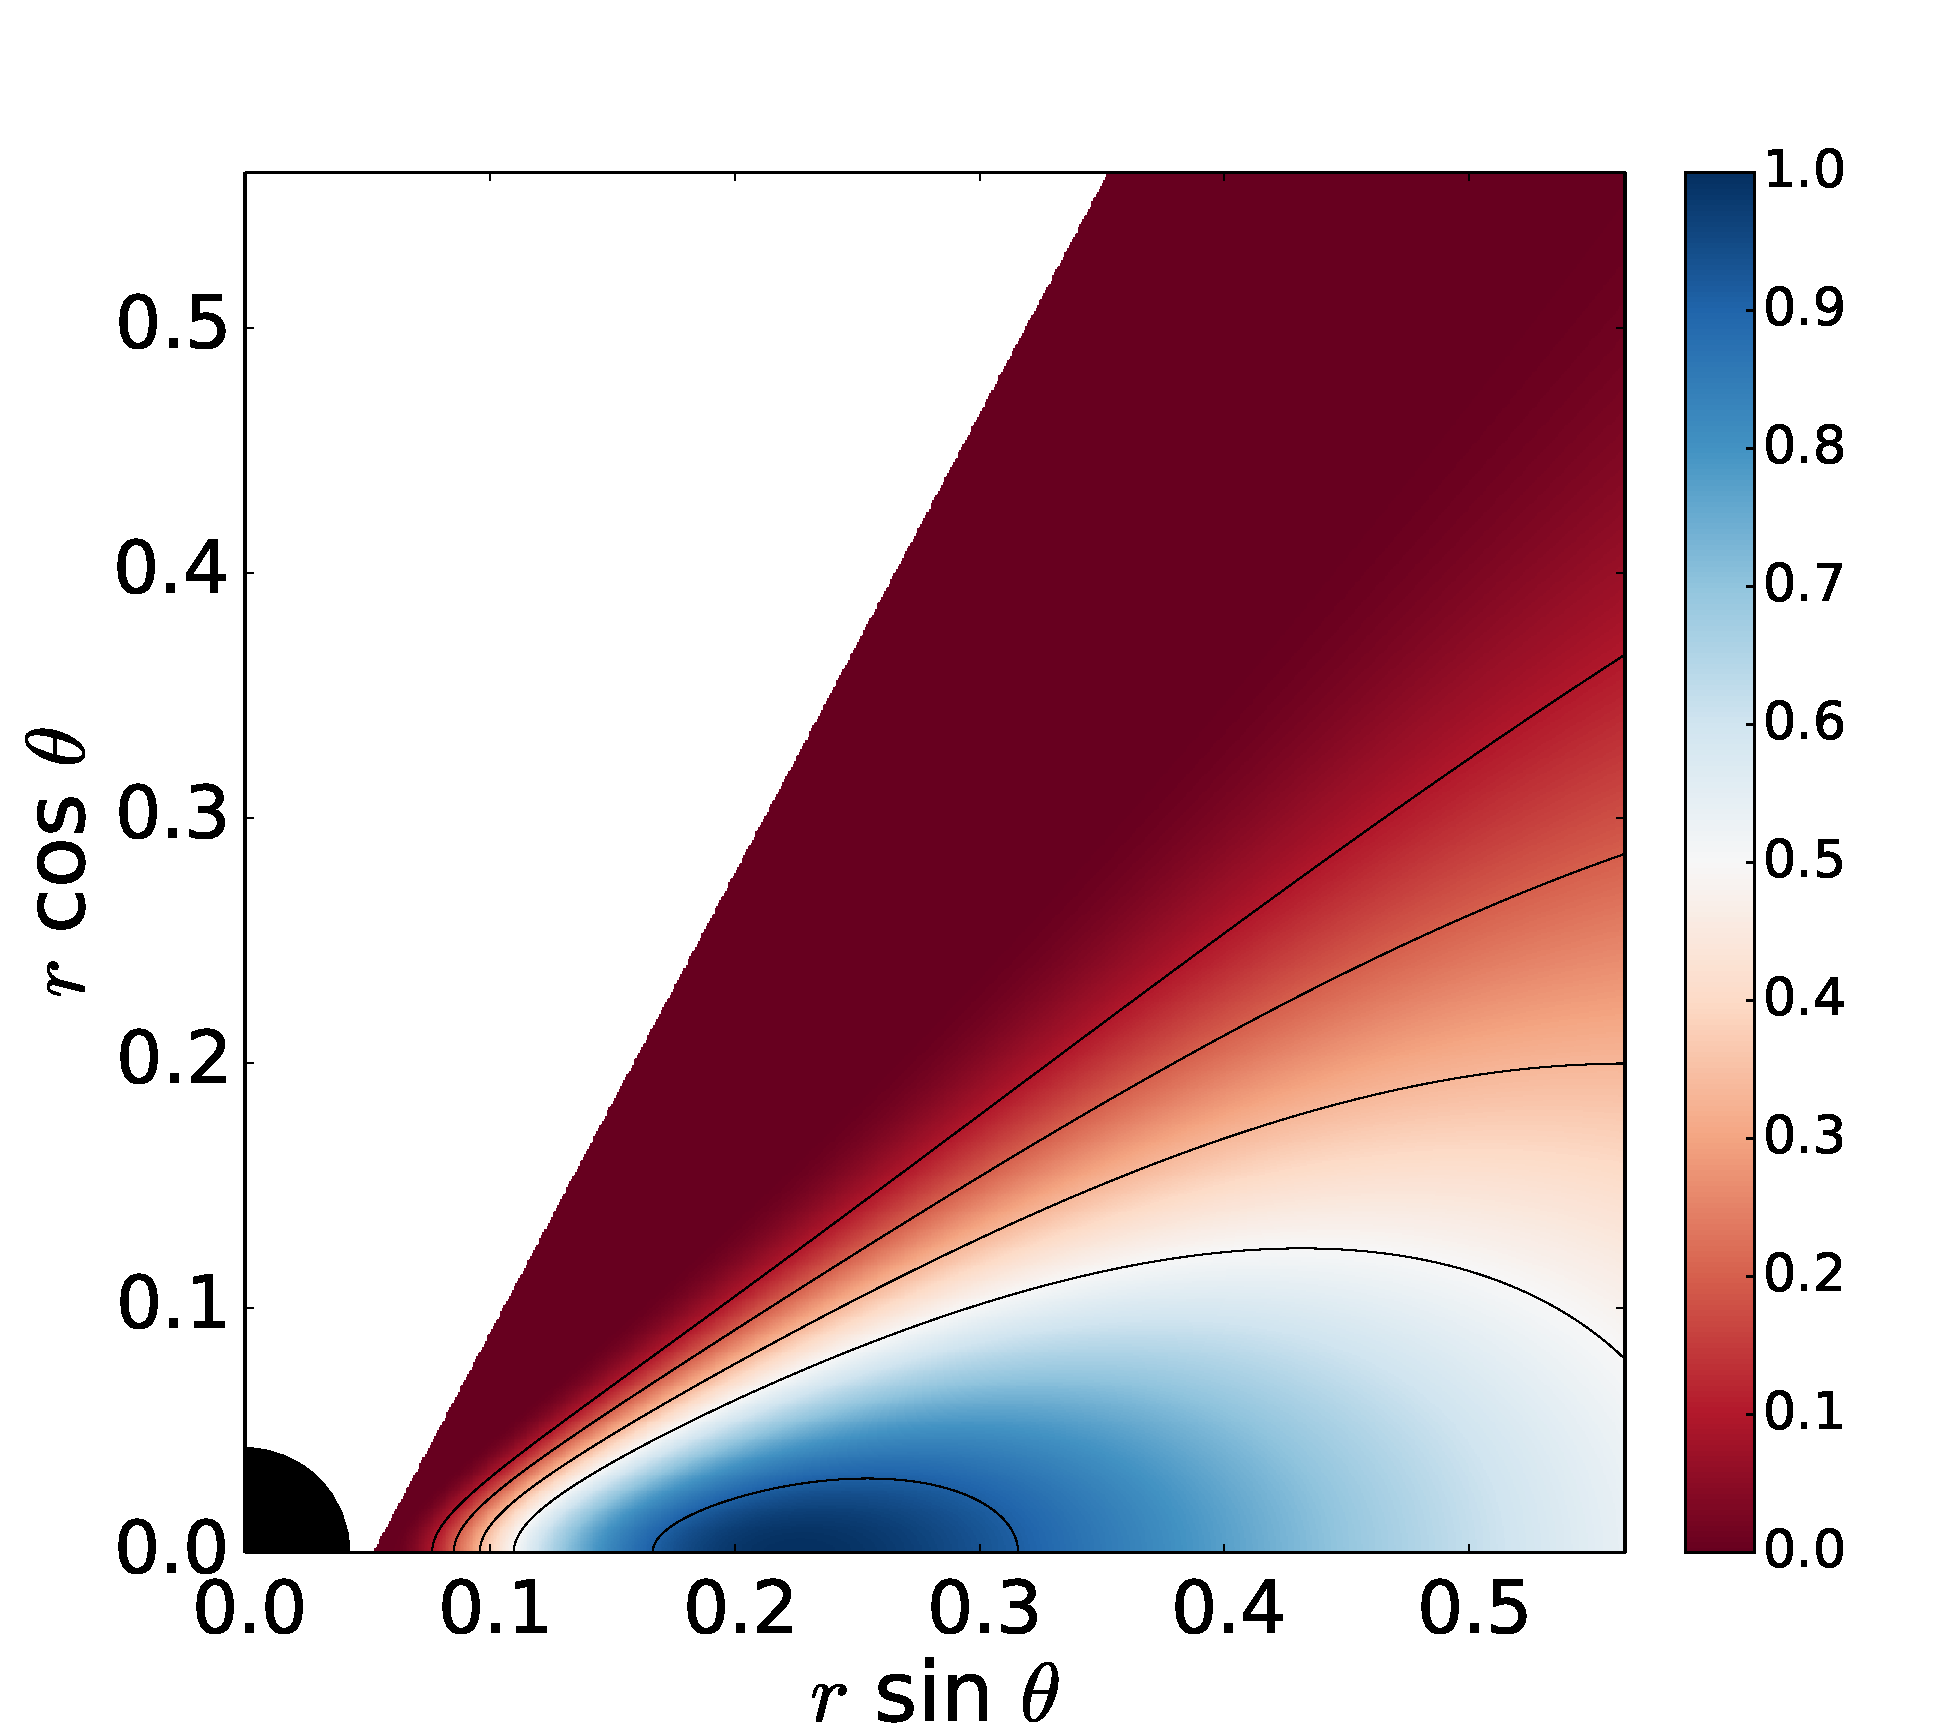
\includegraphics[scale=0.2]{figures/fig2_III_ADM_3.pdf}
\hspace{-0.2cm}
\\
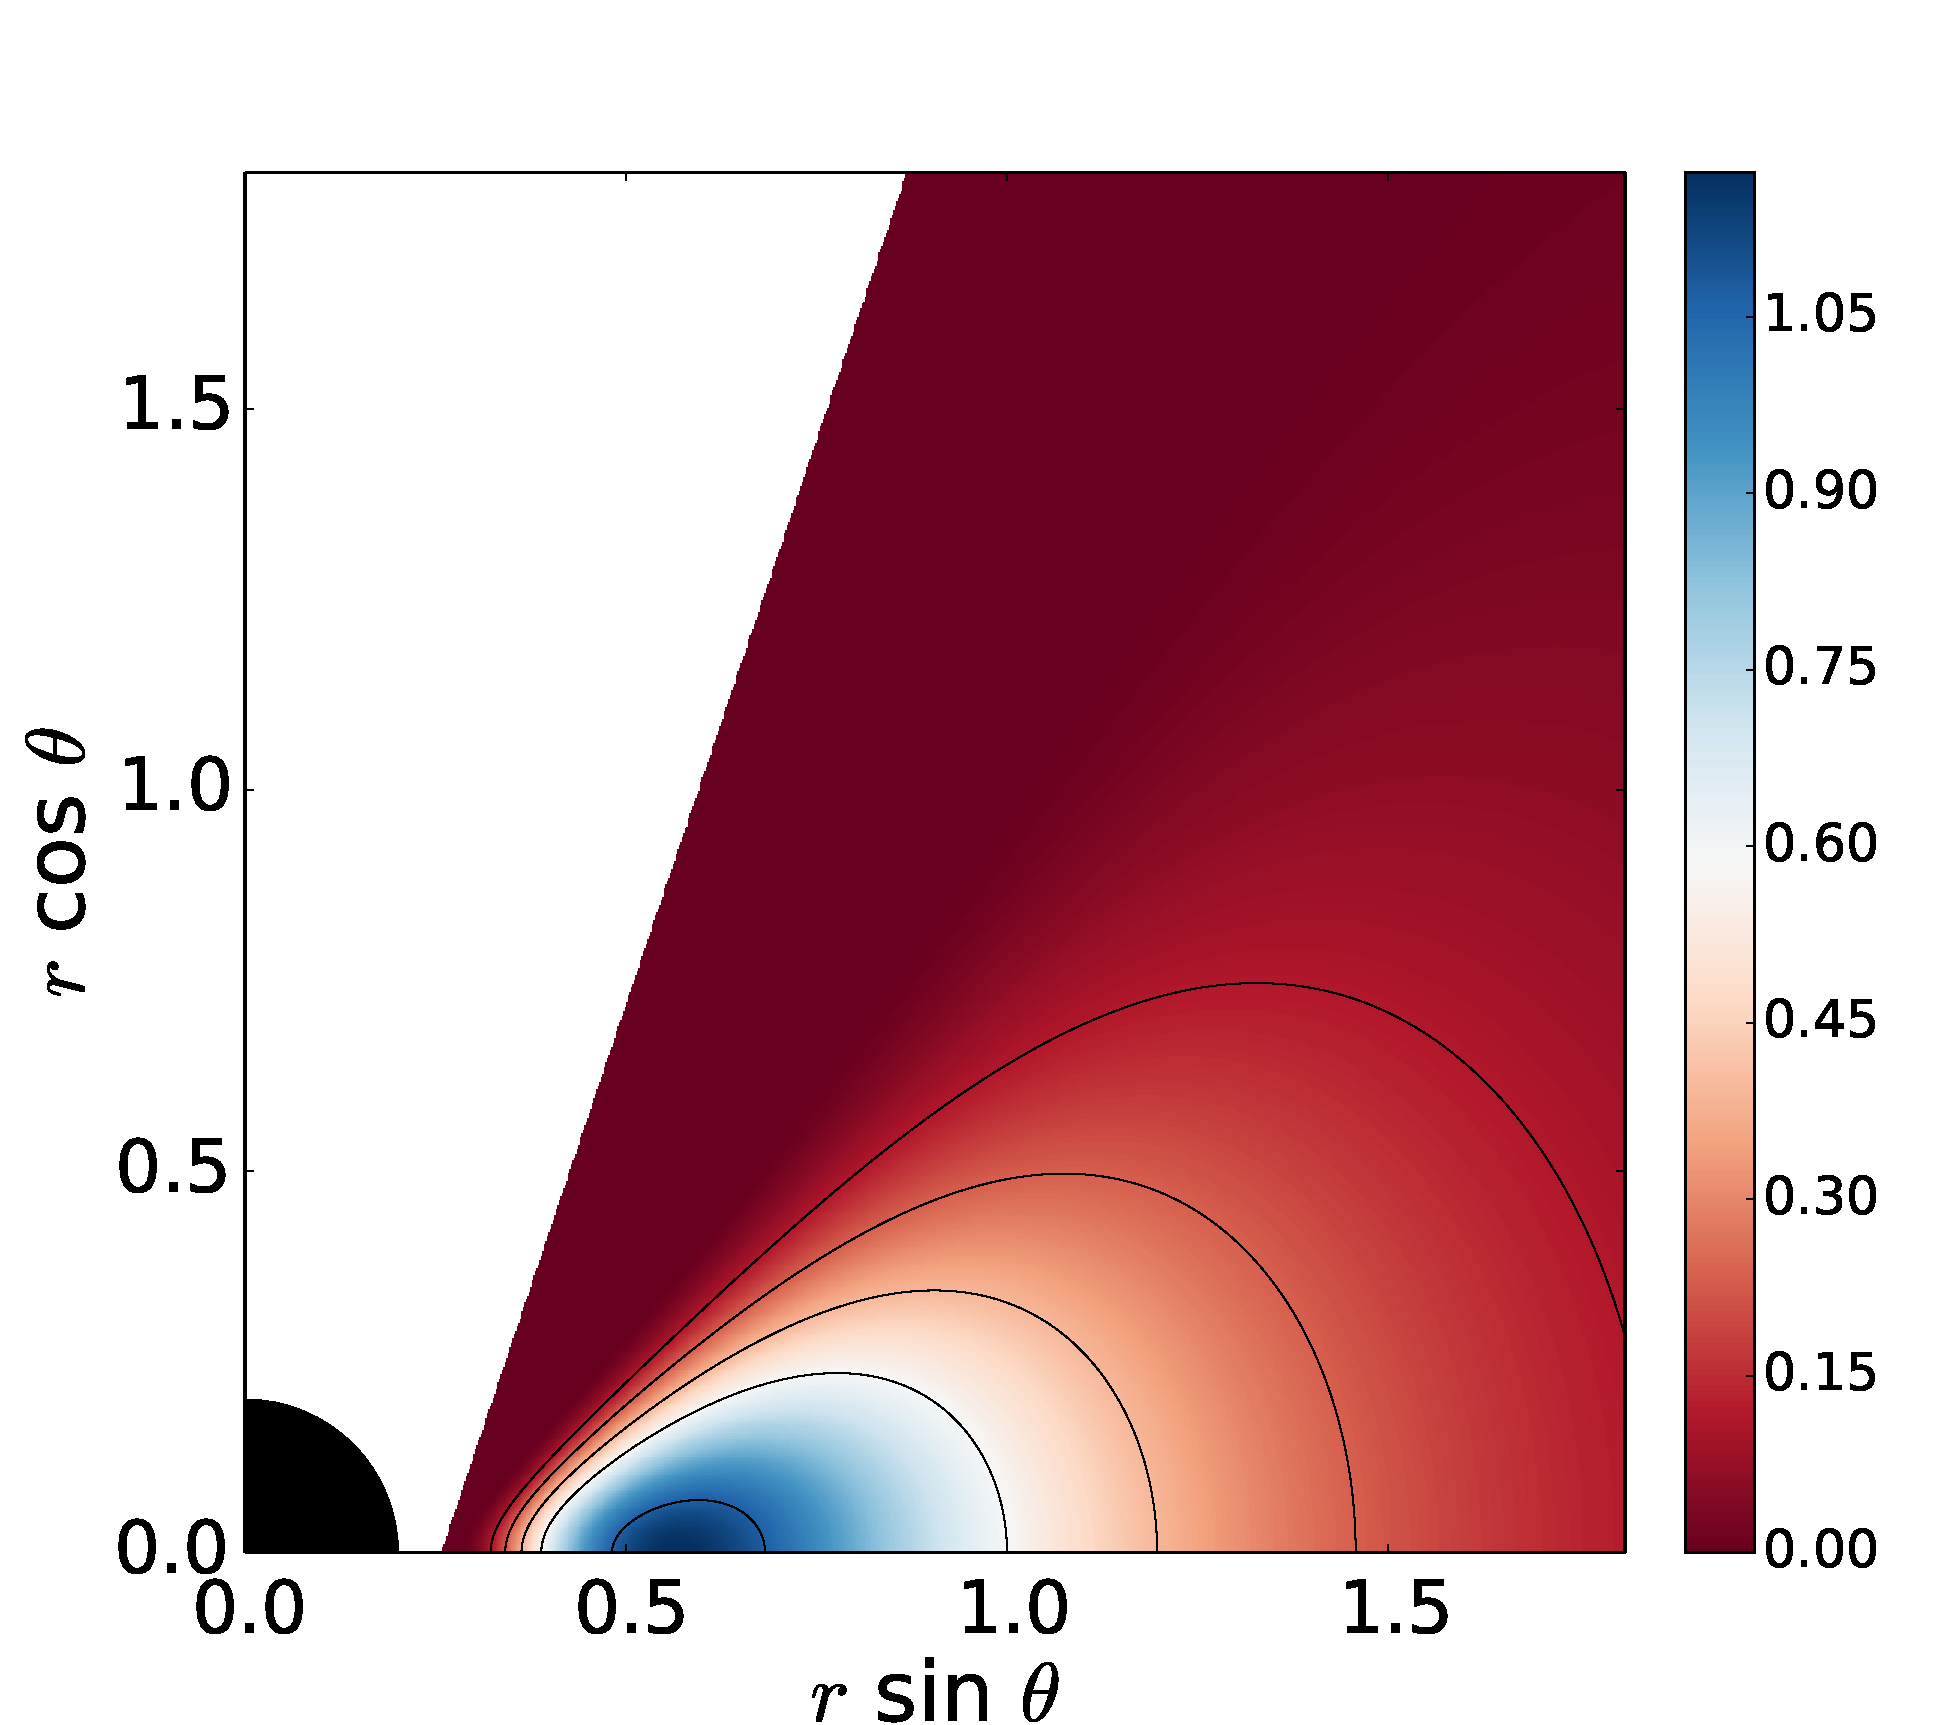
\includegraphics[scale=0.2]{figures/fig2_III_HBH_0.pdf}
\hspace{-0.3cm}
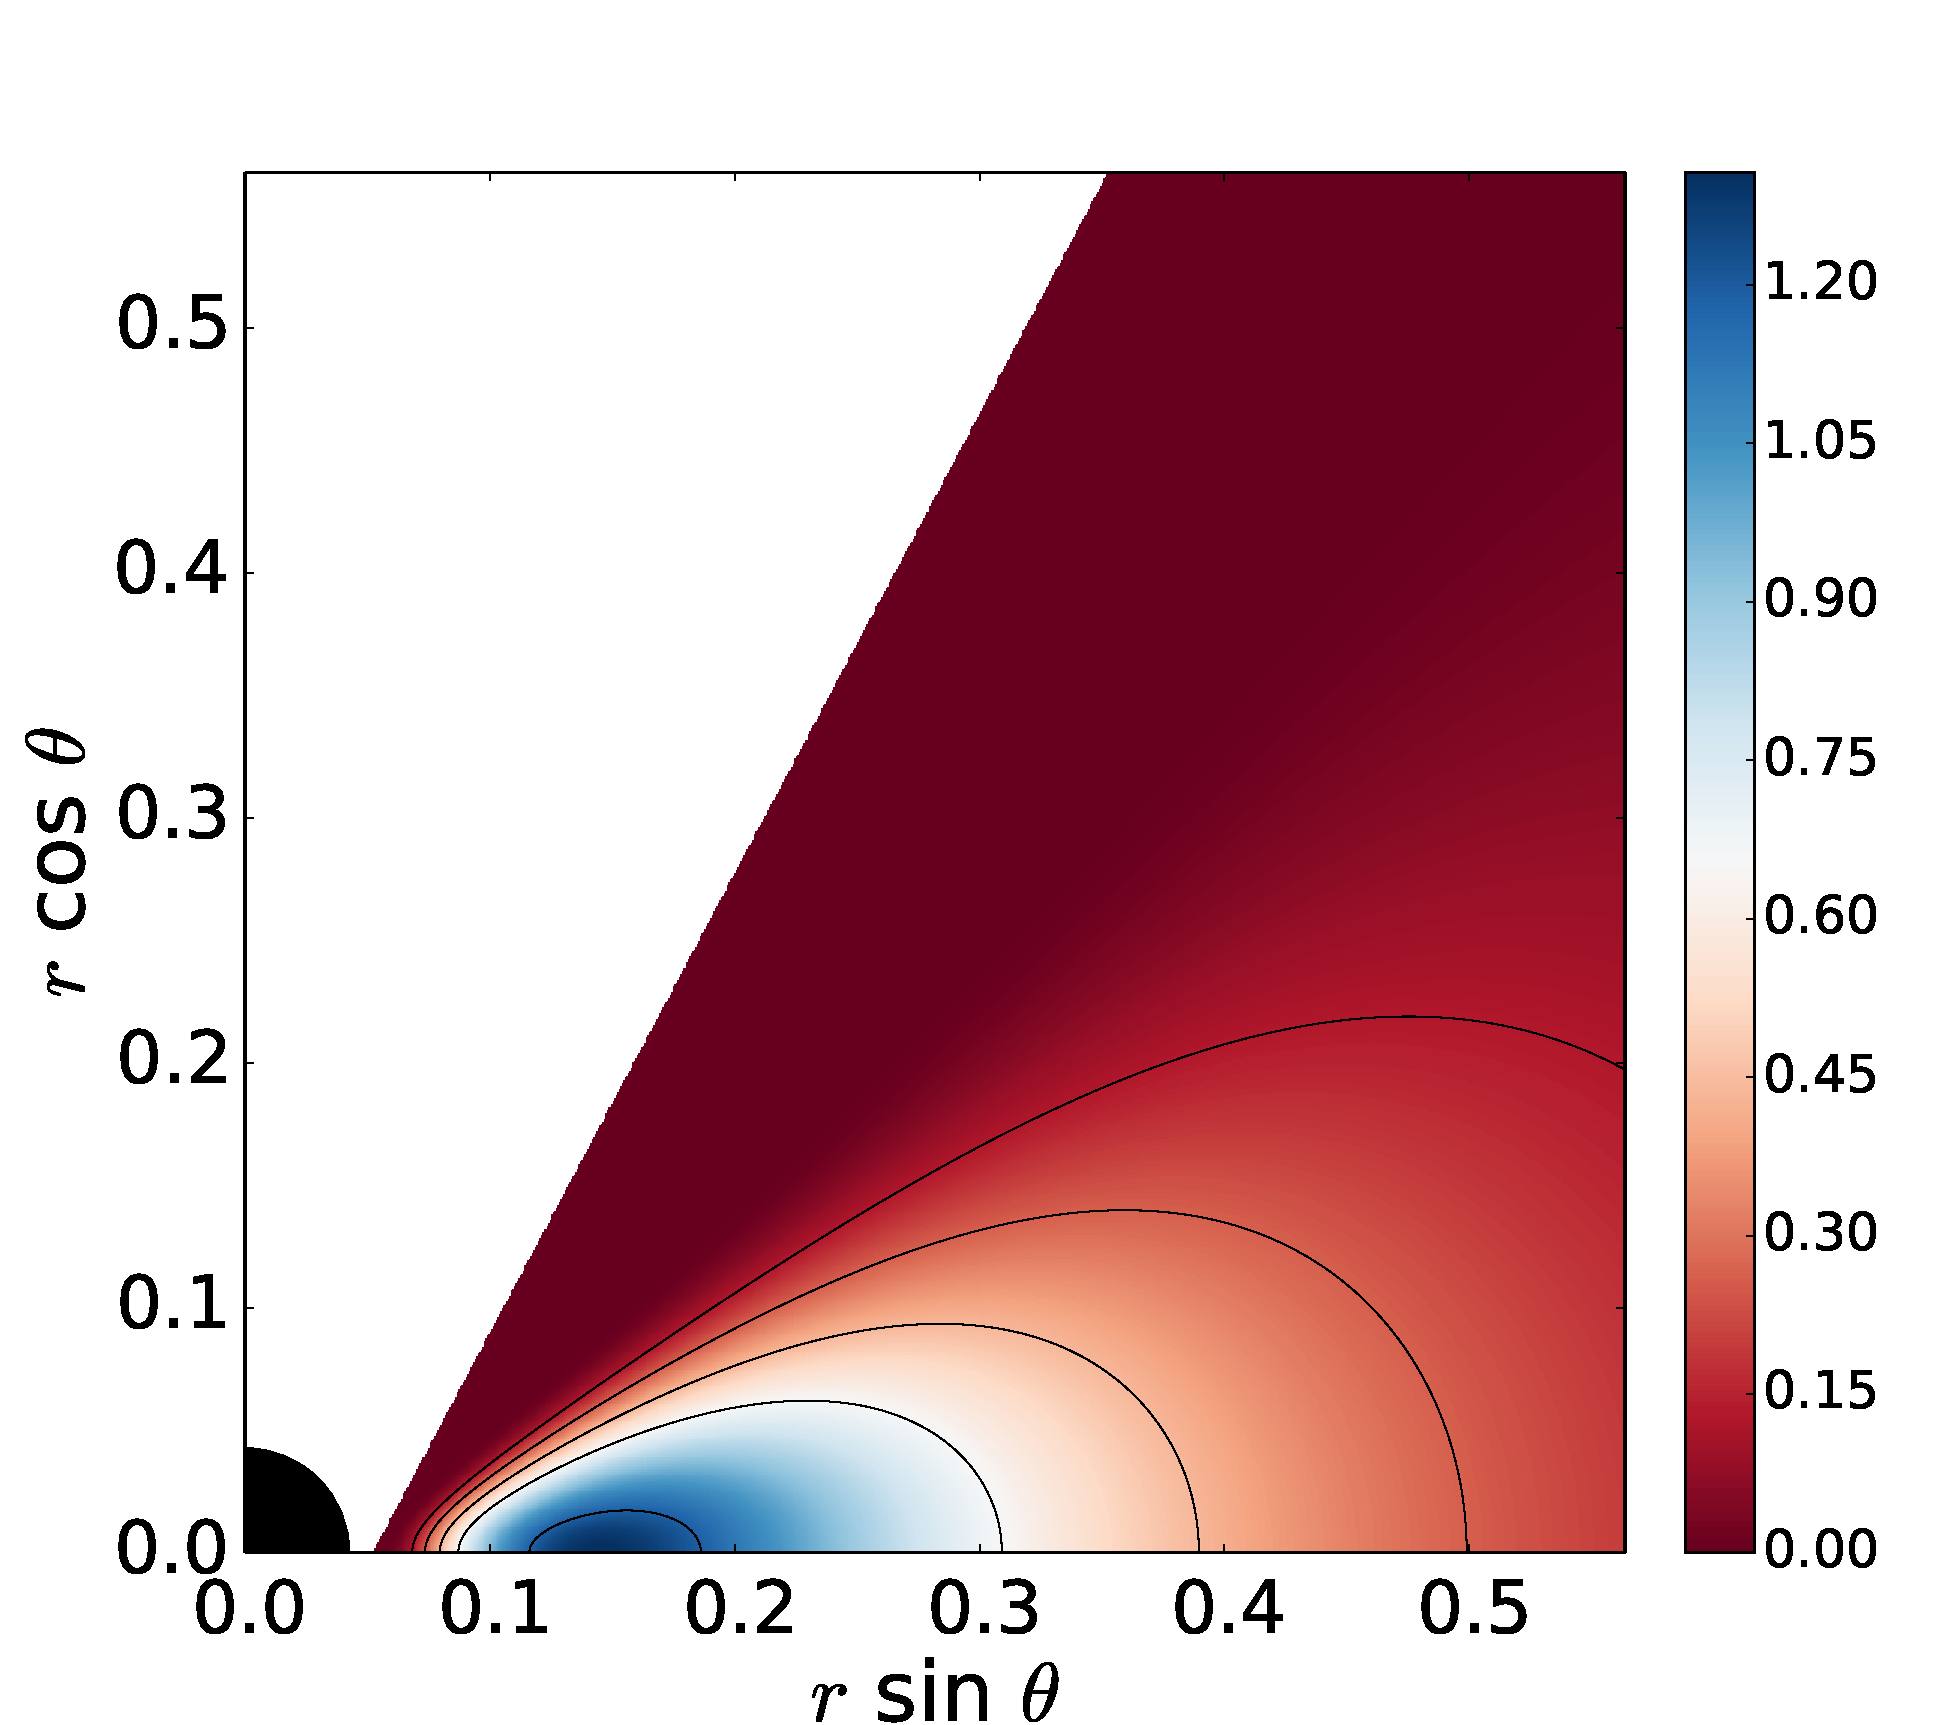
\includegraphics[scale=0.2]{figures/fig2_III_ADM_0.pdf}
\hspace{-0.2cm}
\\
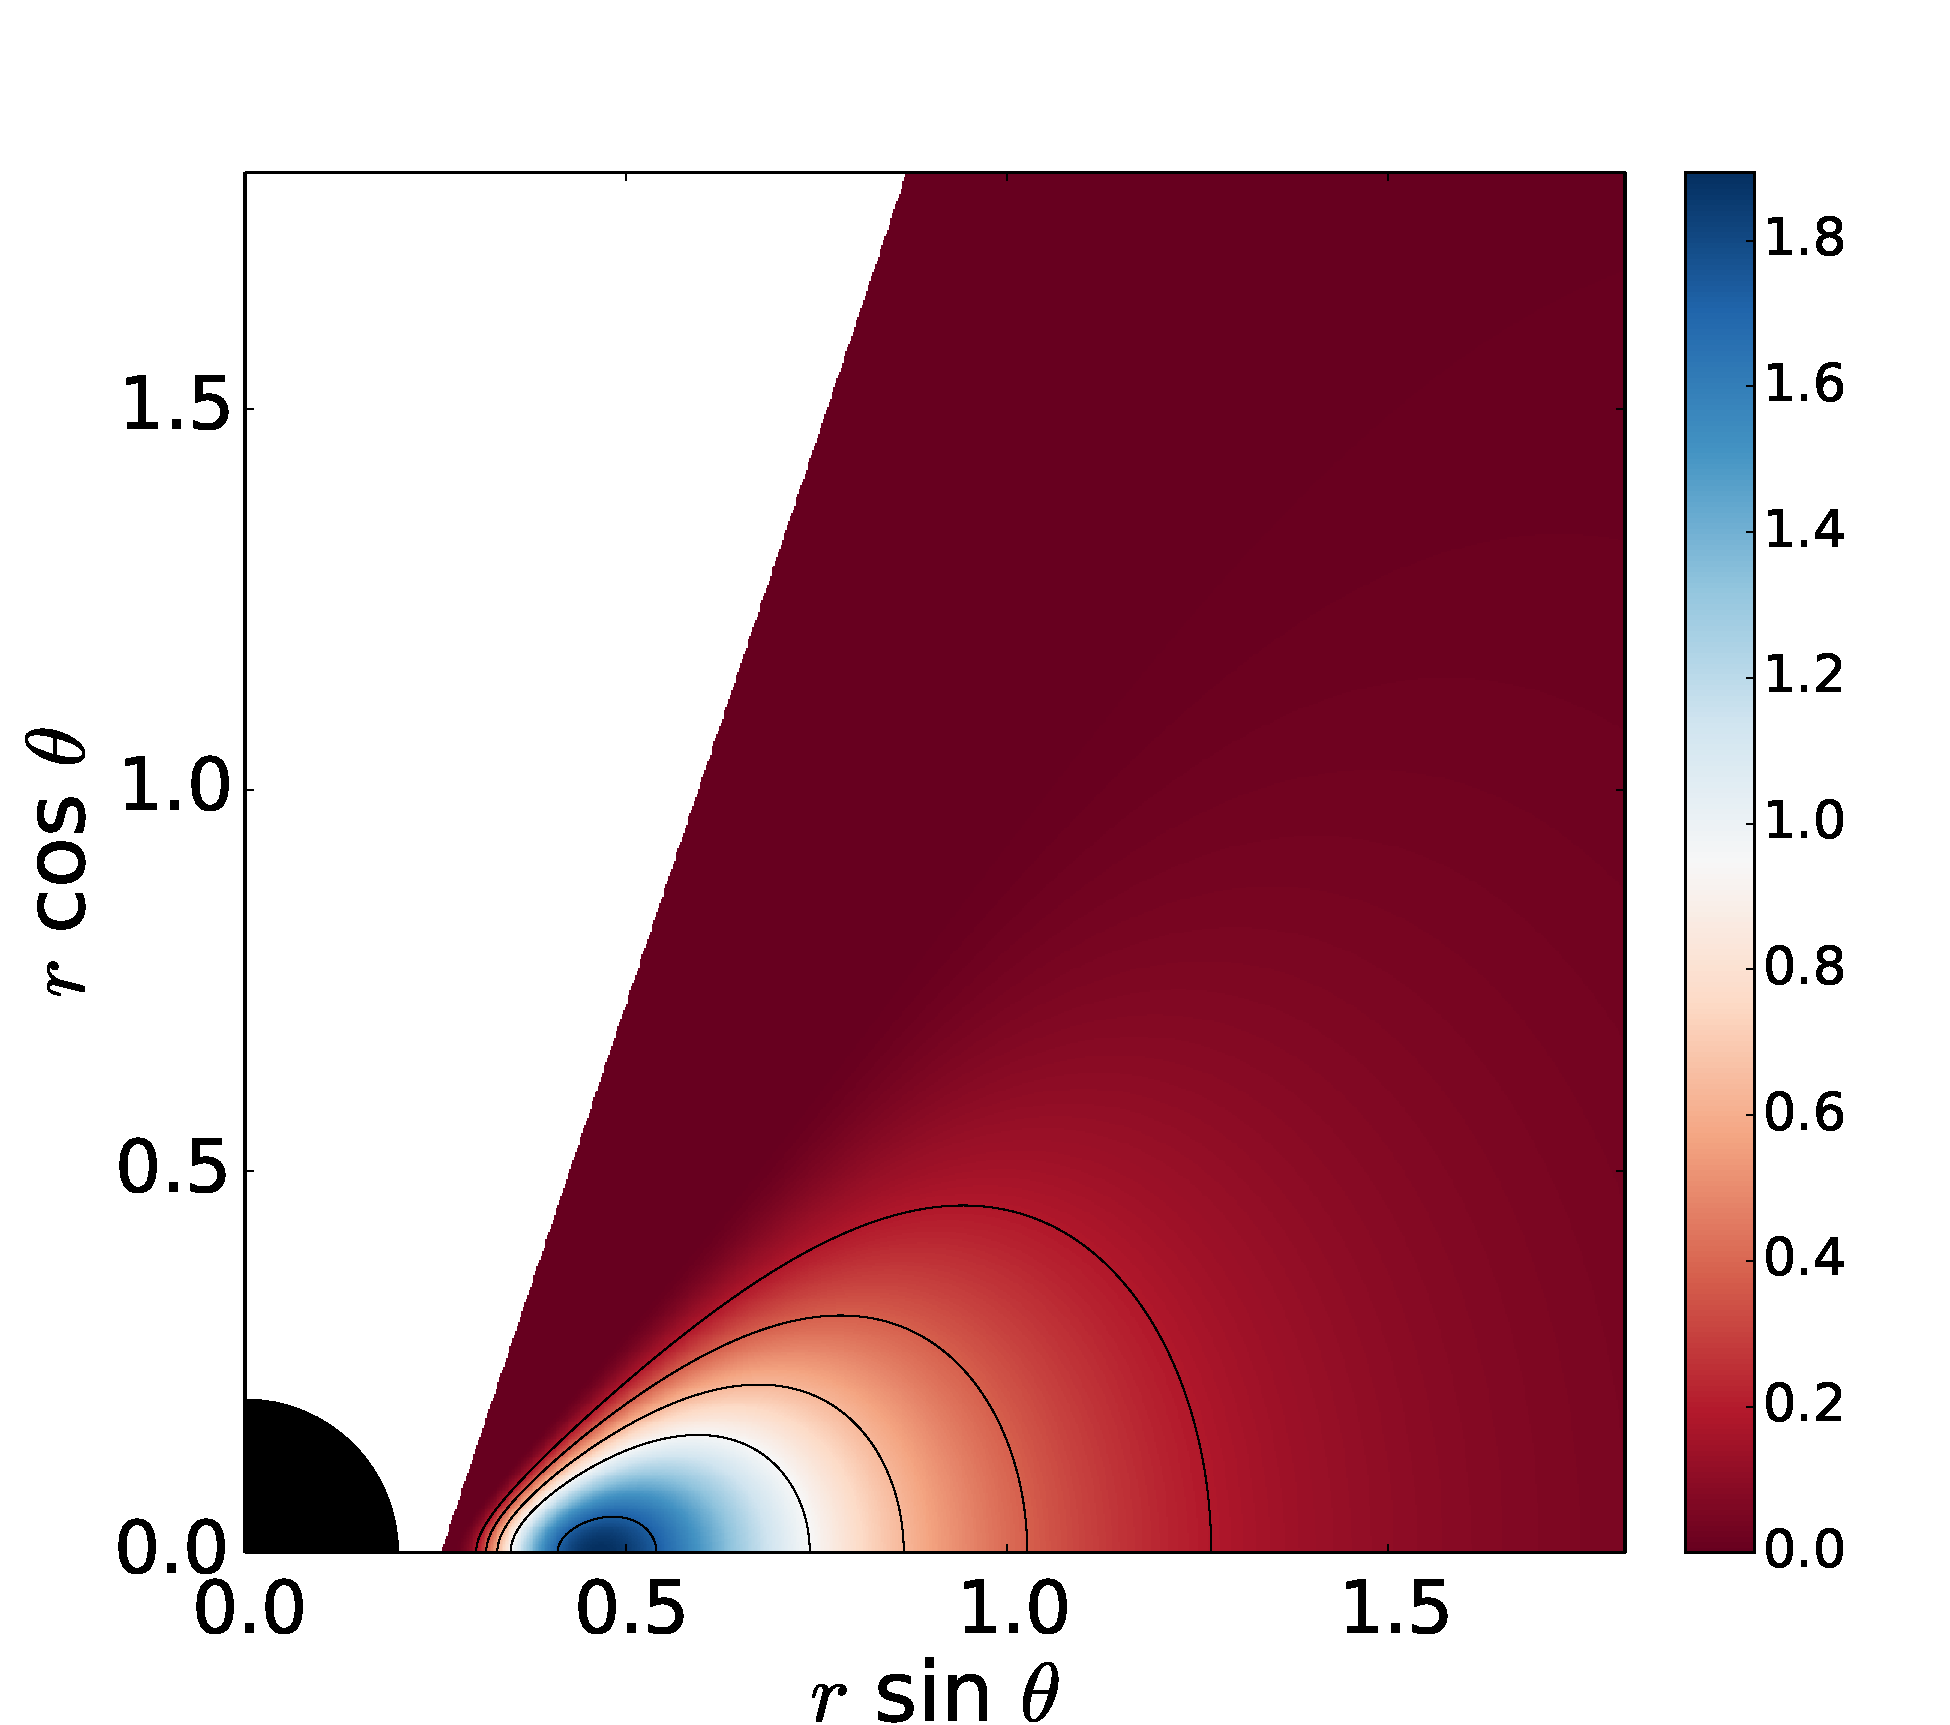
\includegraphics[scale=0.2]{figures/fig2_III_HBH__3.pdf}
\hspace{-0.3cm}
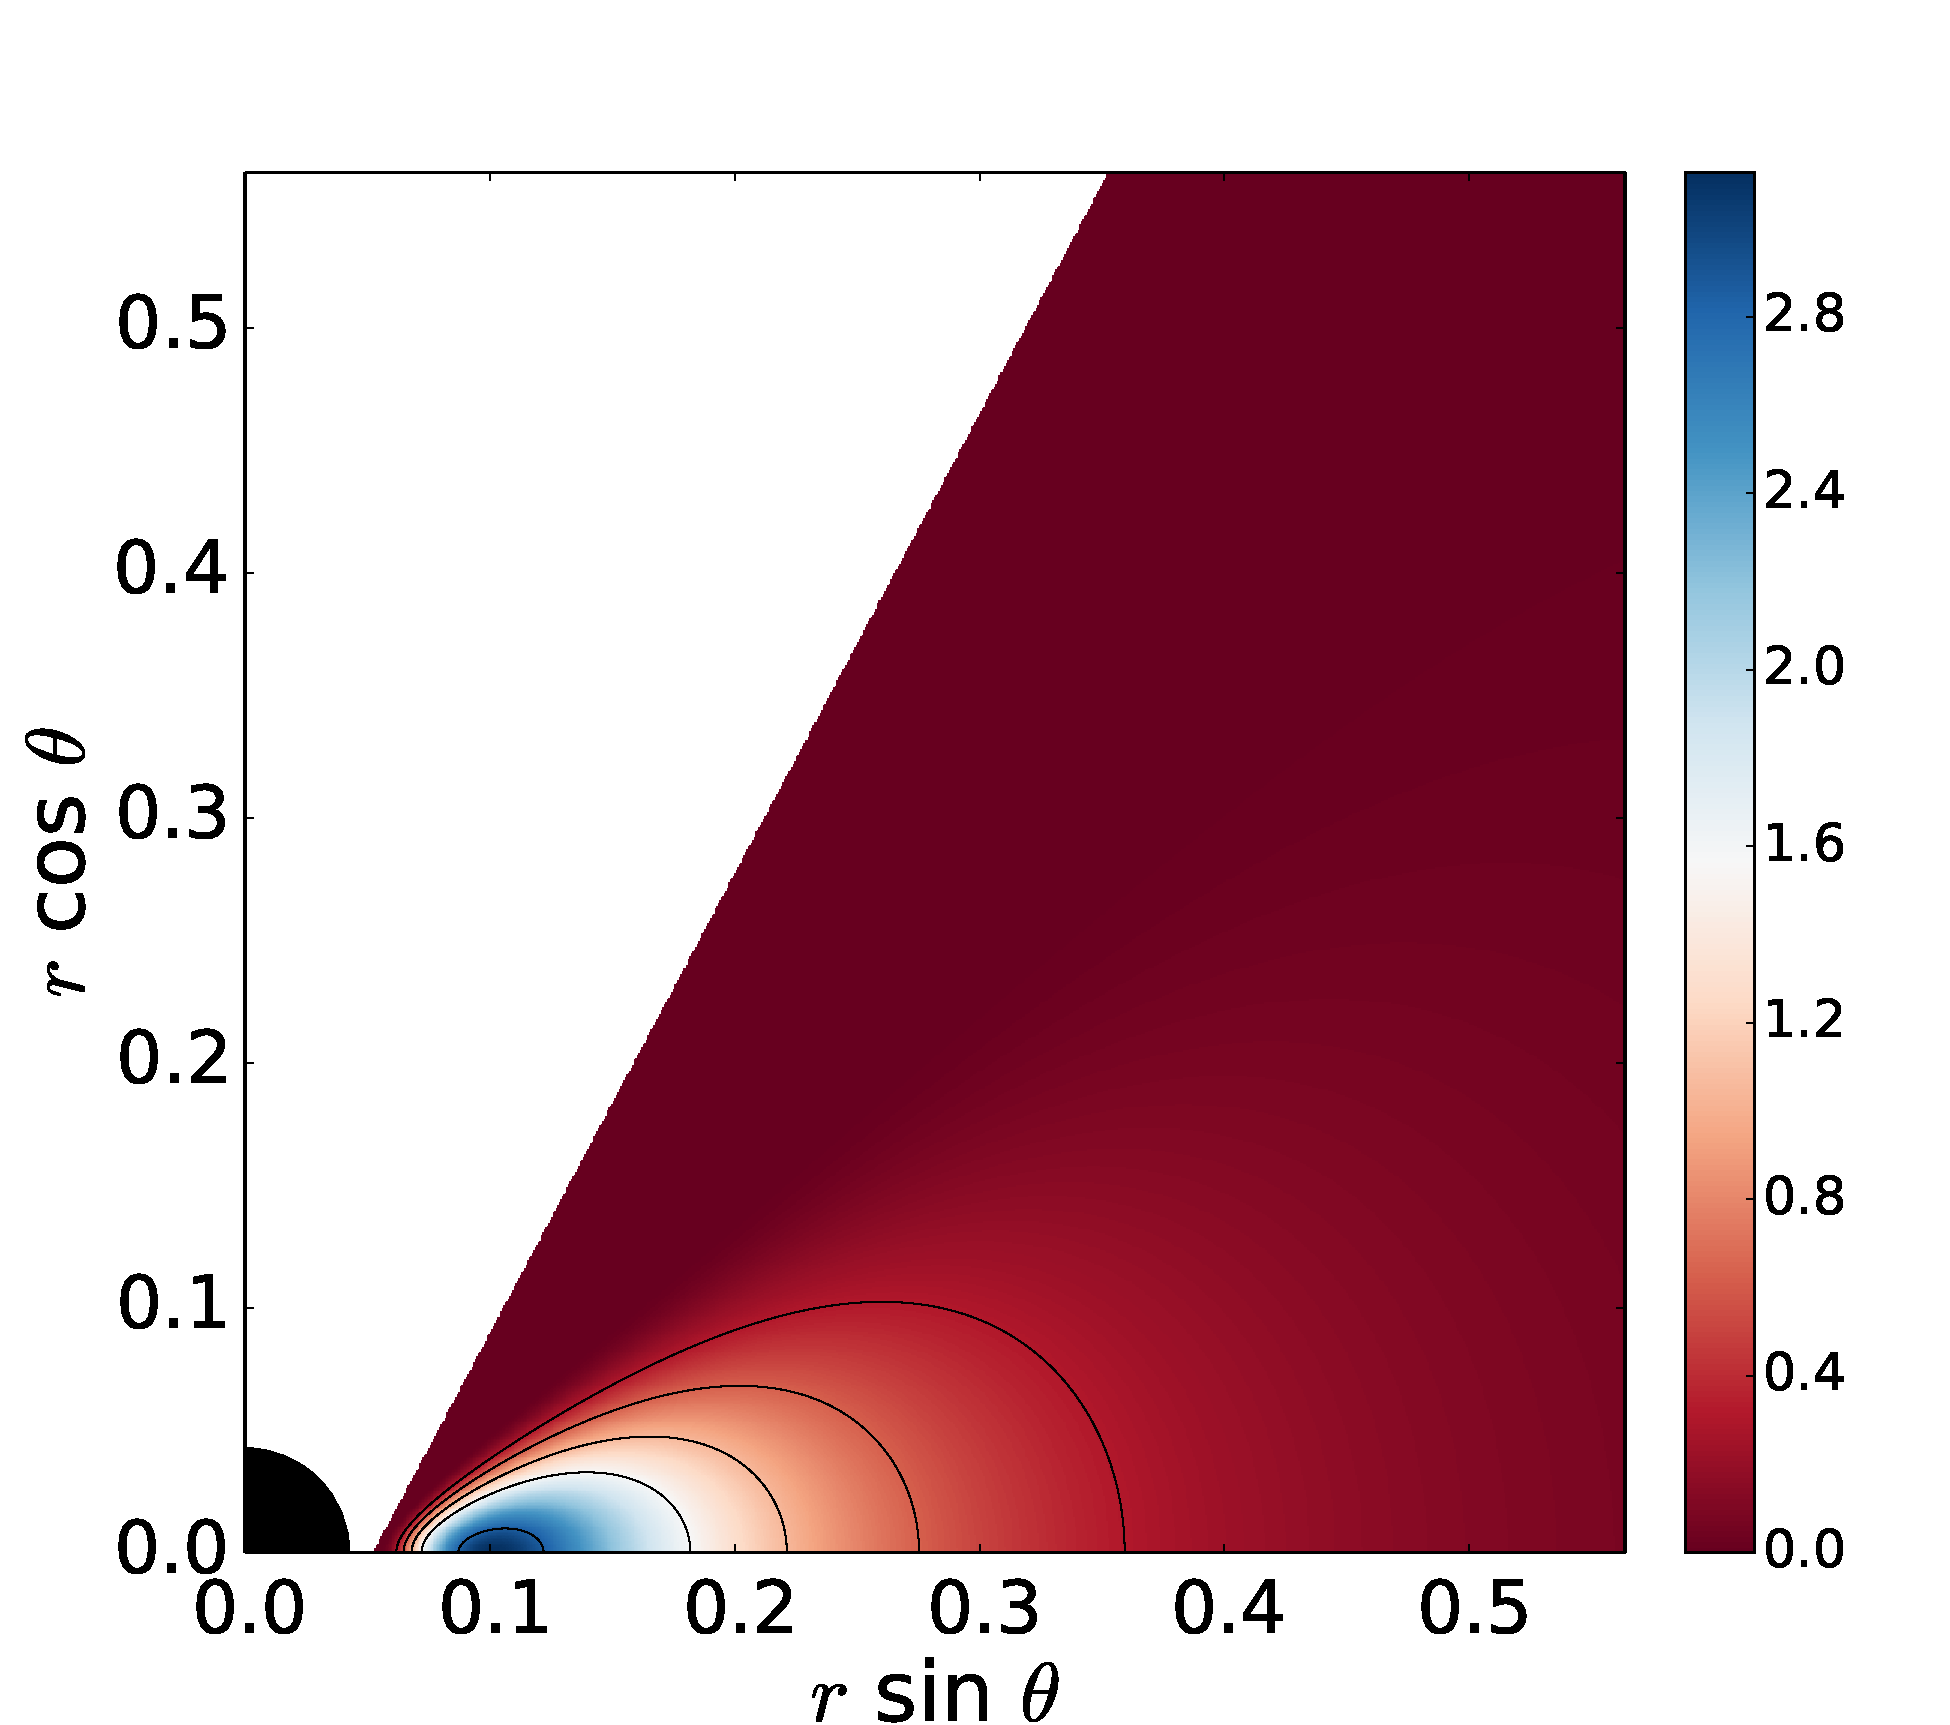
\includegraphics[scale=0.2]{figures/fig2_III_ADM__3.pdf}
\hspace{-0.2cm}
\caption{Rest-mass density distribution for the model I. From top to bottom the rows correspond to the different values of the magnetization parameter, namely non-magnetized ($\beta_{\mathrm{m}_{\mathrm{c}}} = 10^{3}$), mildly magnetized ($\beta_{\mathrm{m}_{\mathrm{c}}} = 1$) and strongly magnetized ($\beta_{\mathrm{m}_{\mathrm{c}}} = 10^{-3}$). The left column correspond to the KBHsSH model and the right column correspond to the corresponding KBH with the same ADM quantities.}
\label{comparison_mag_1}
\end{figure*}

\begin{figure*}
\centering
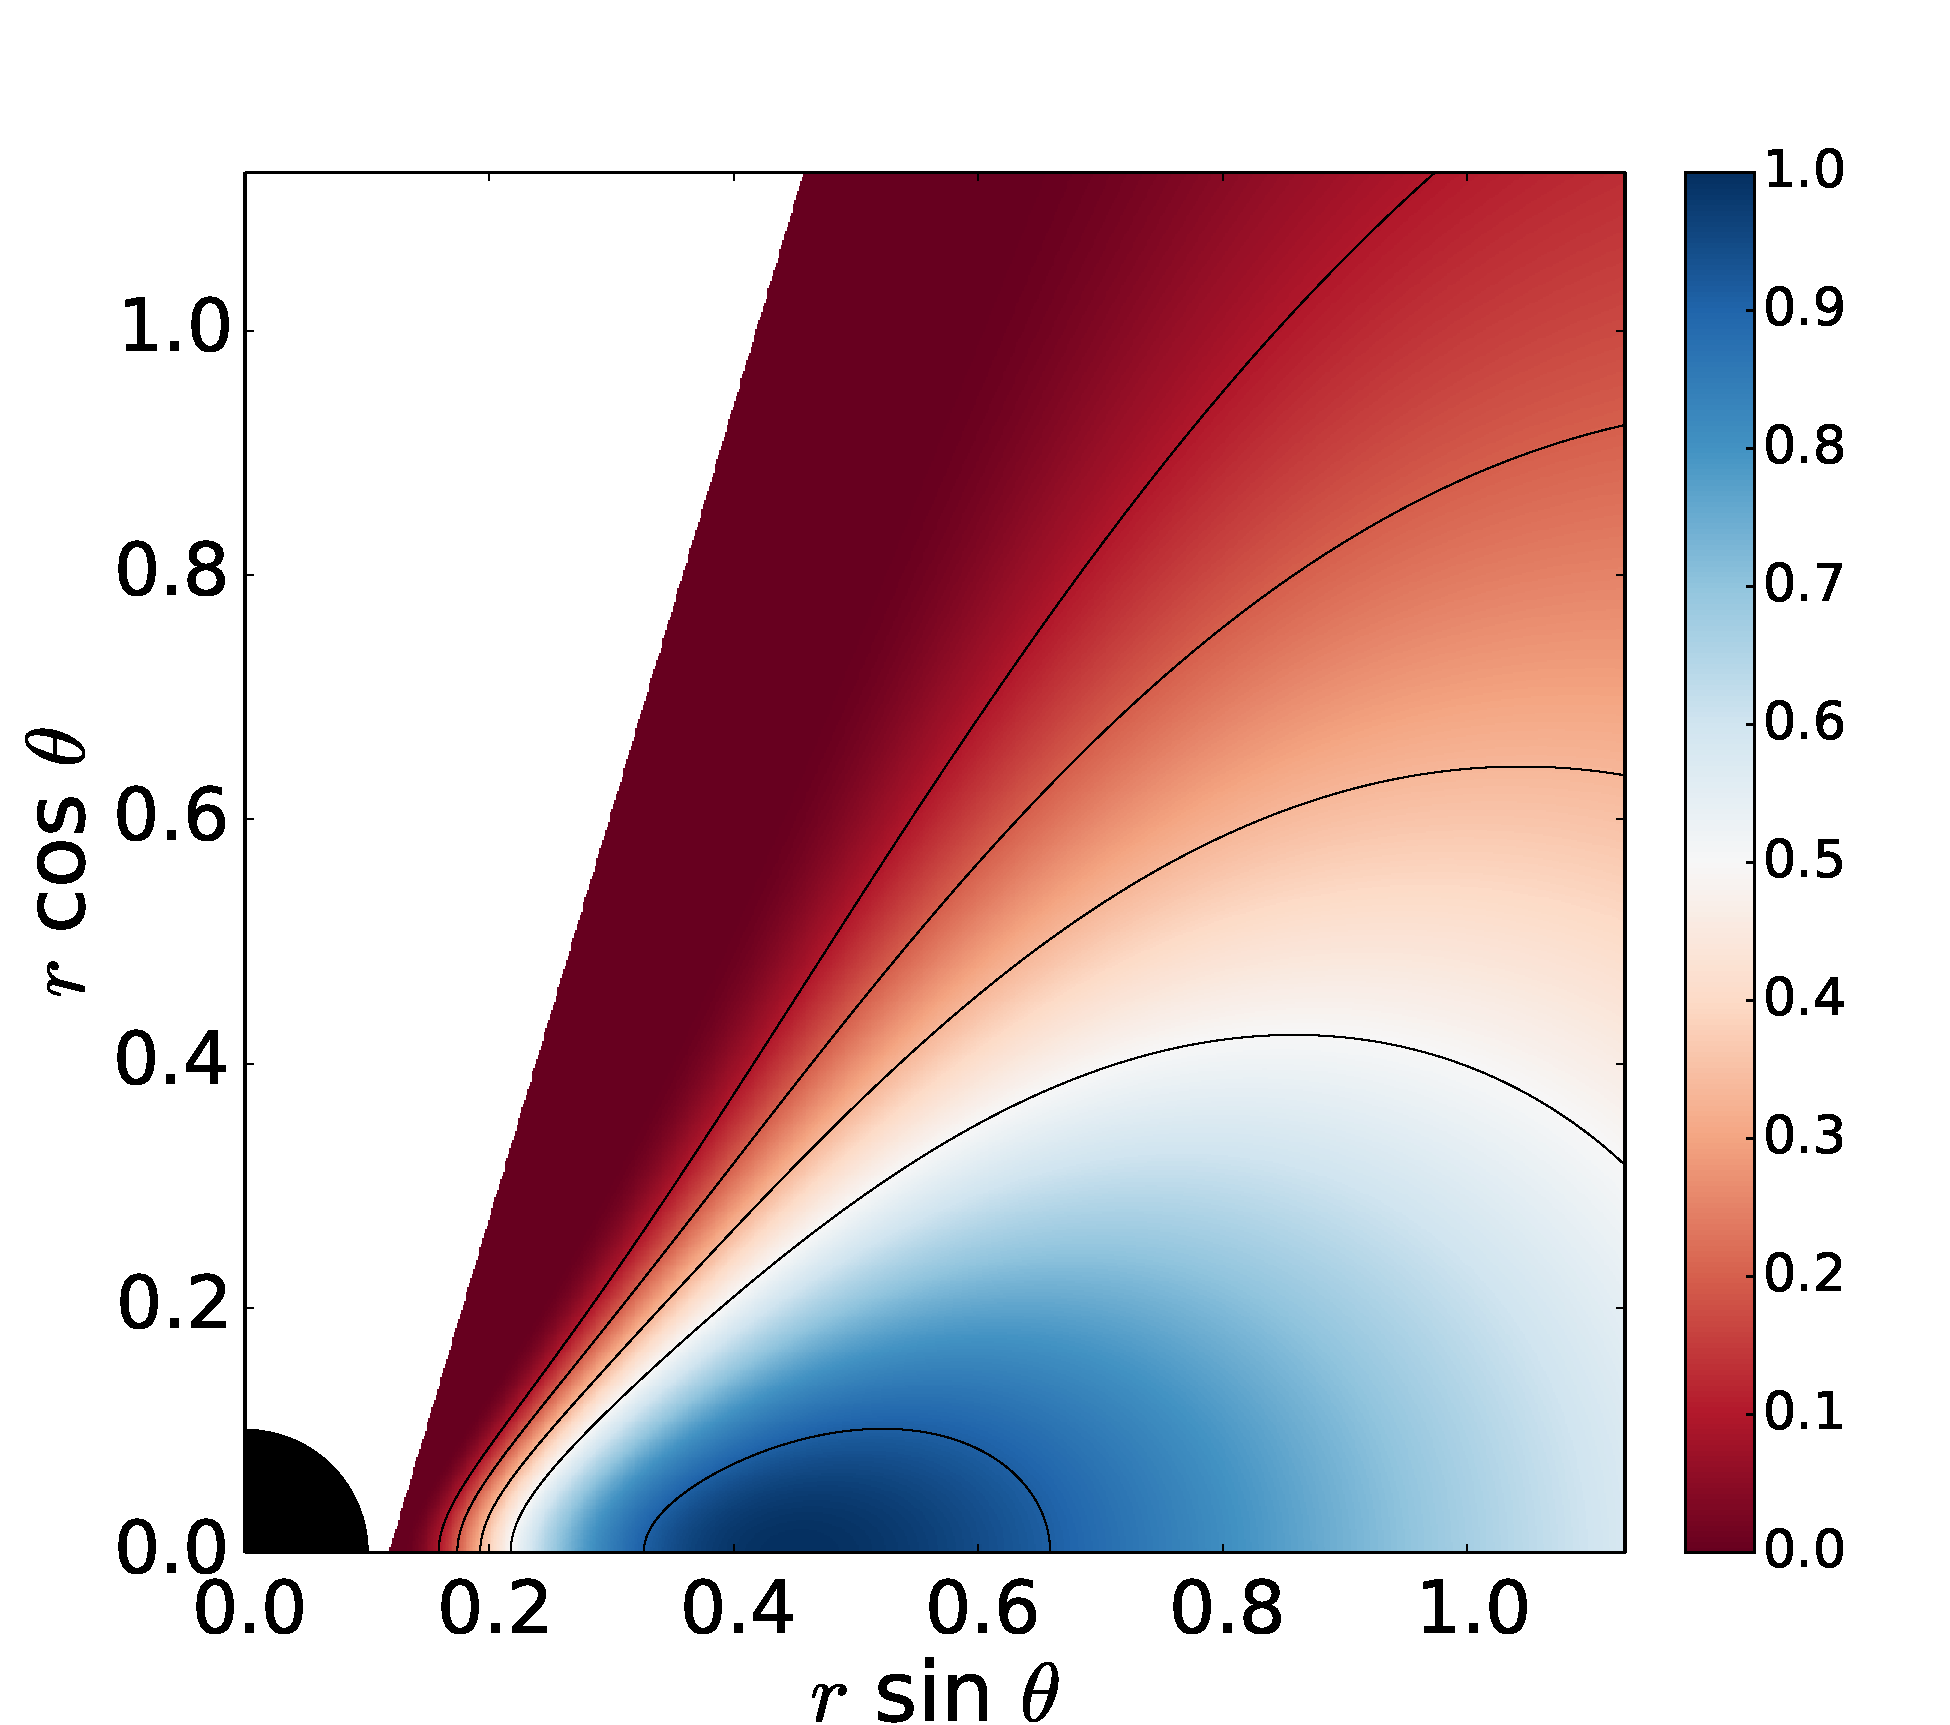
\includegraphics[scale=0.2]{figures/fig3_IV_HBH_3.pdf}
\hspace{-0.3cm}
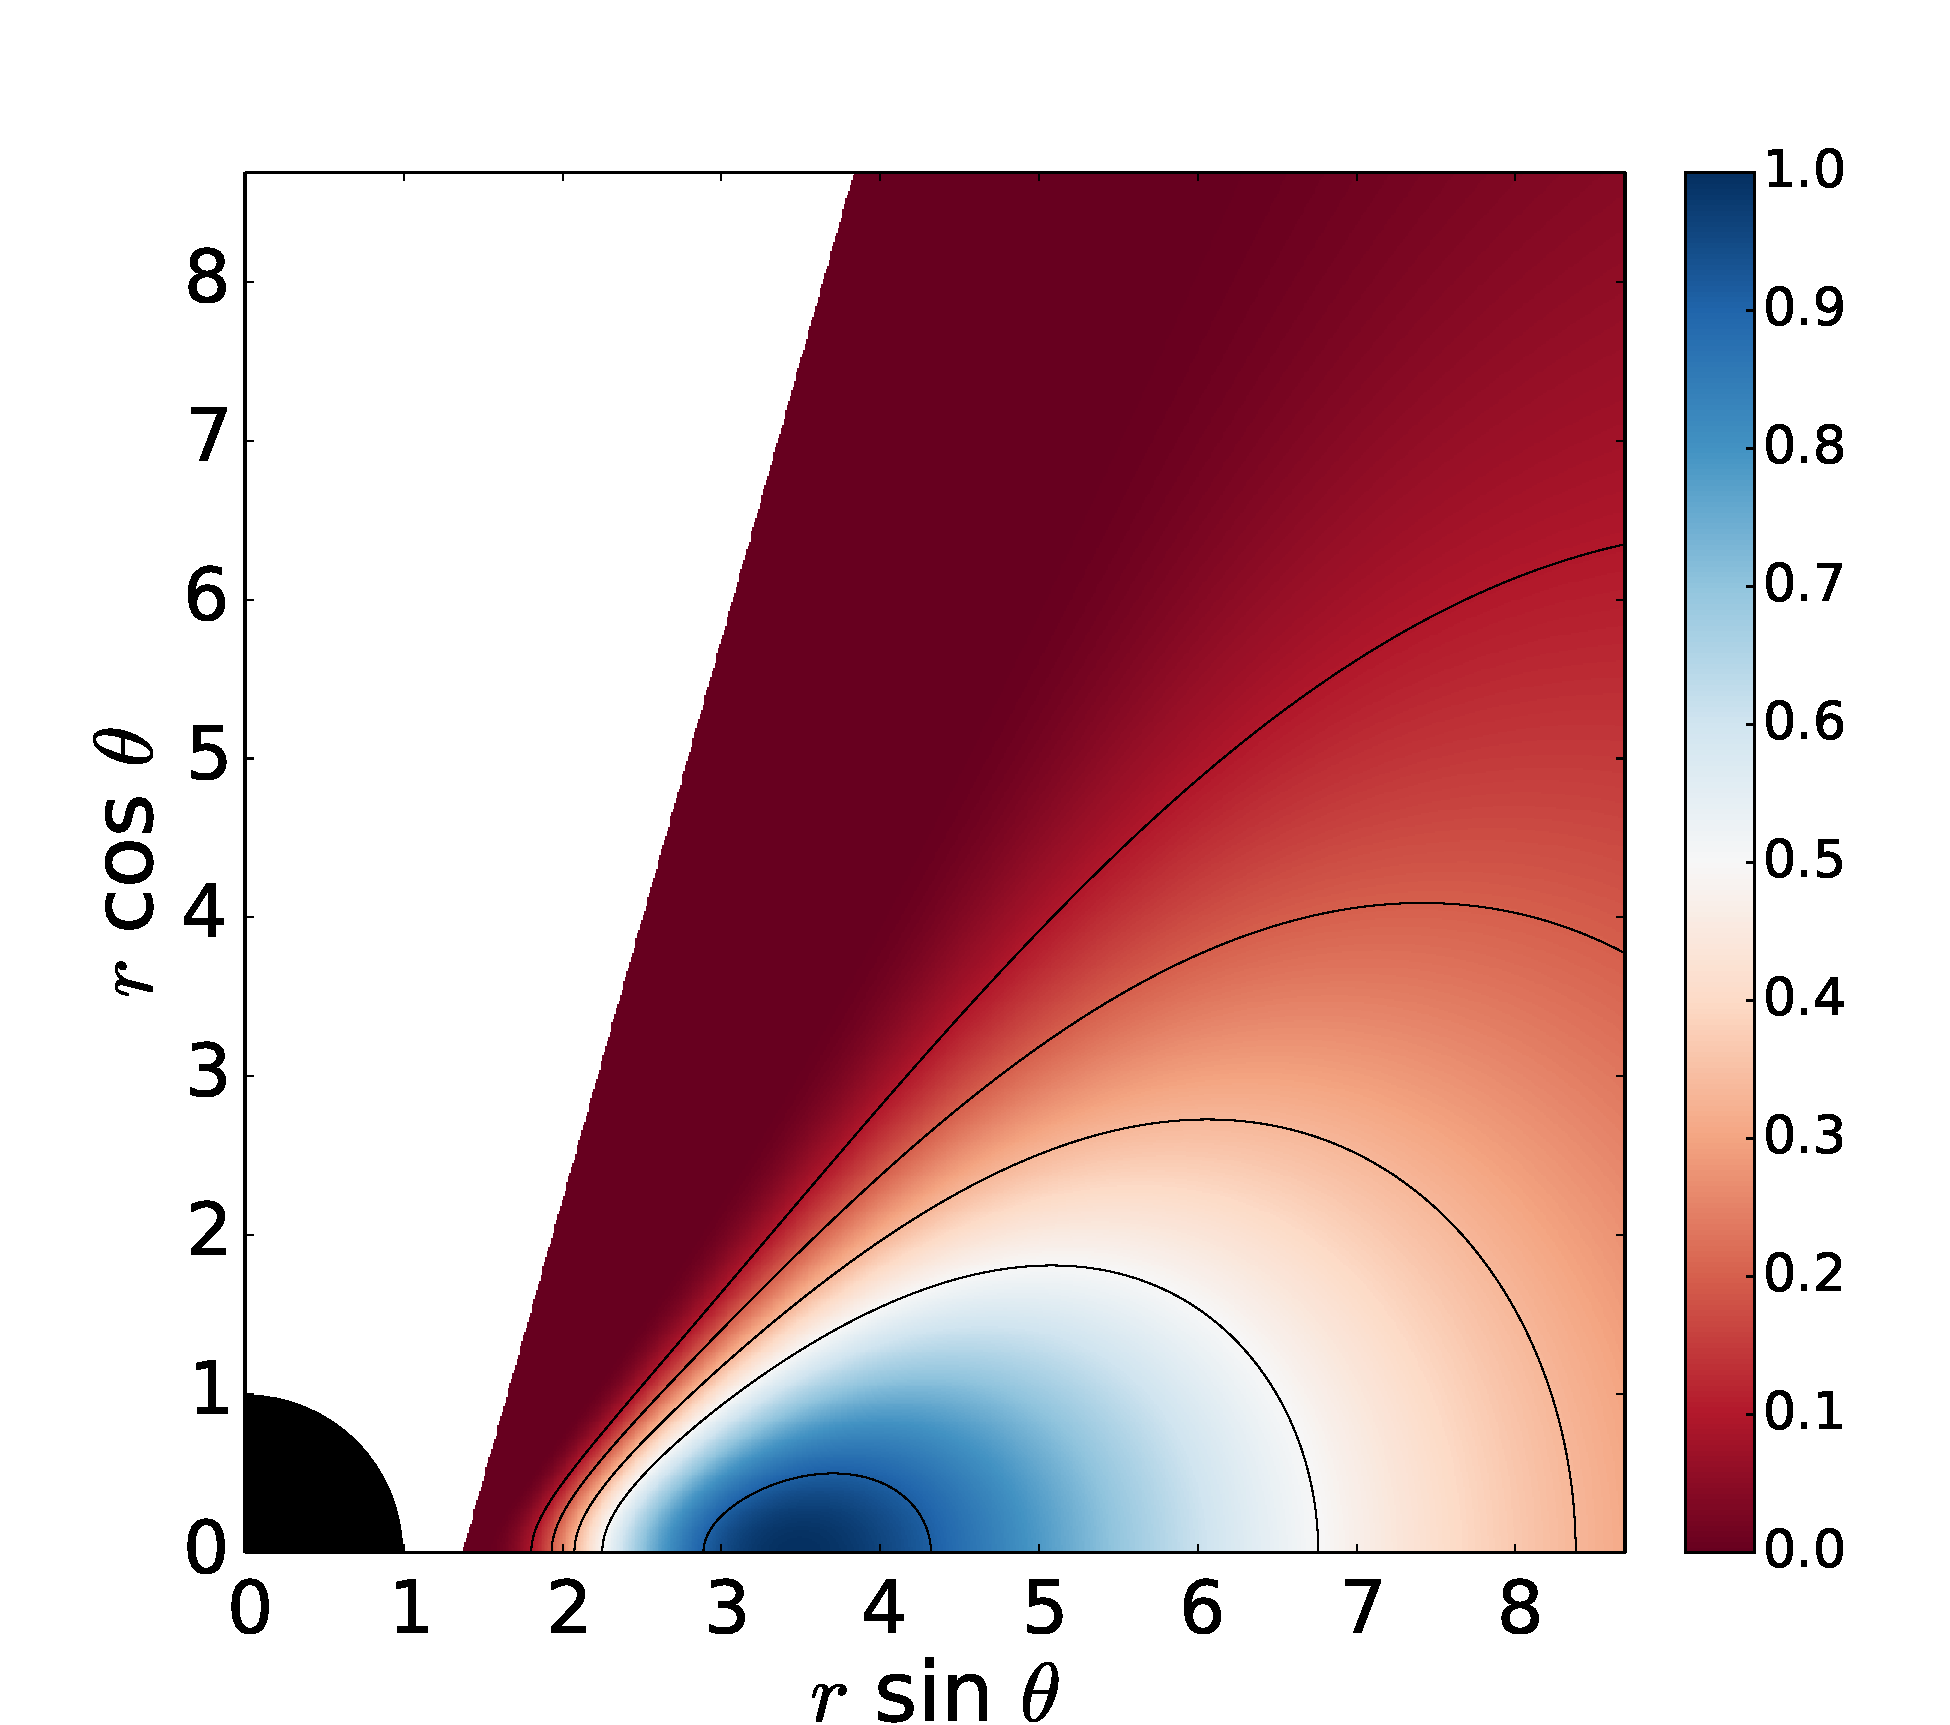
\includegraphics[scale=0.2]{figures/fig3_IV_ADM_3.pdf}
\hspace{-0.2cm}
\\
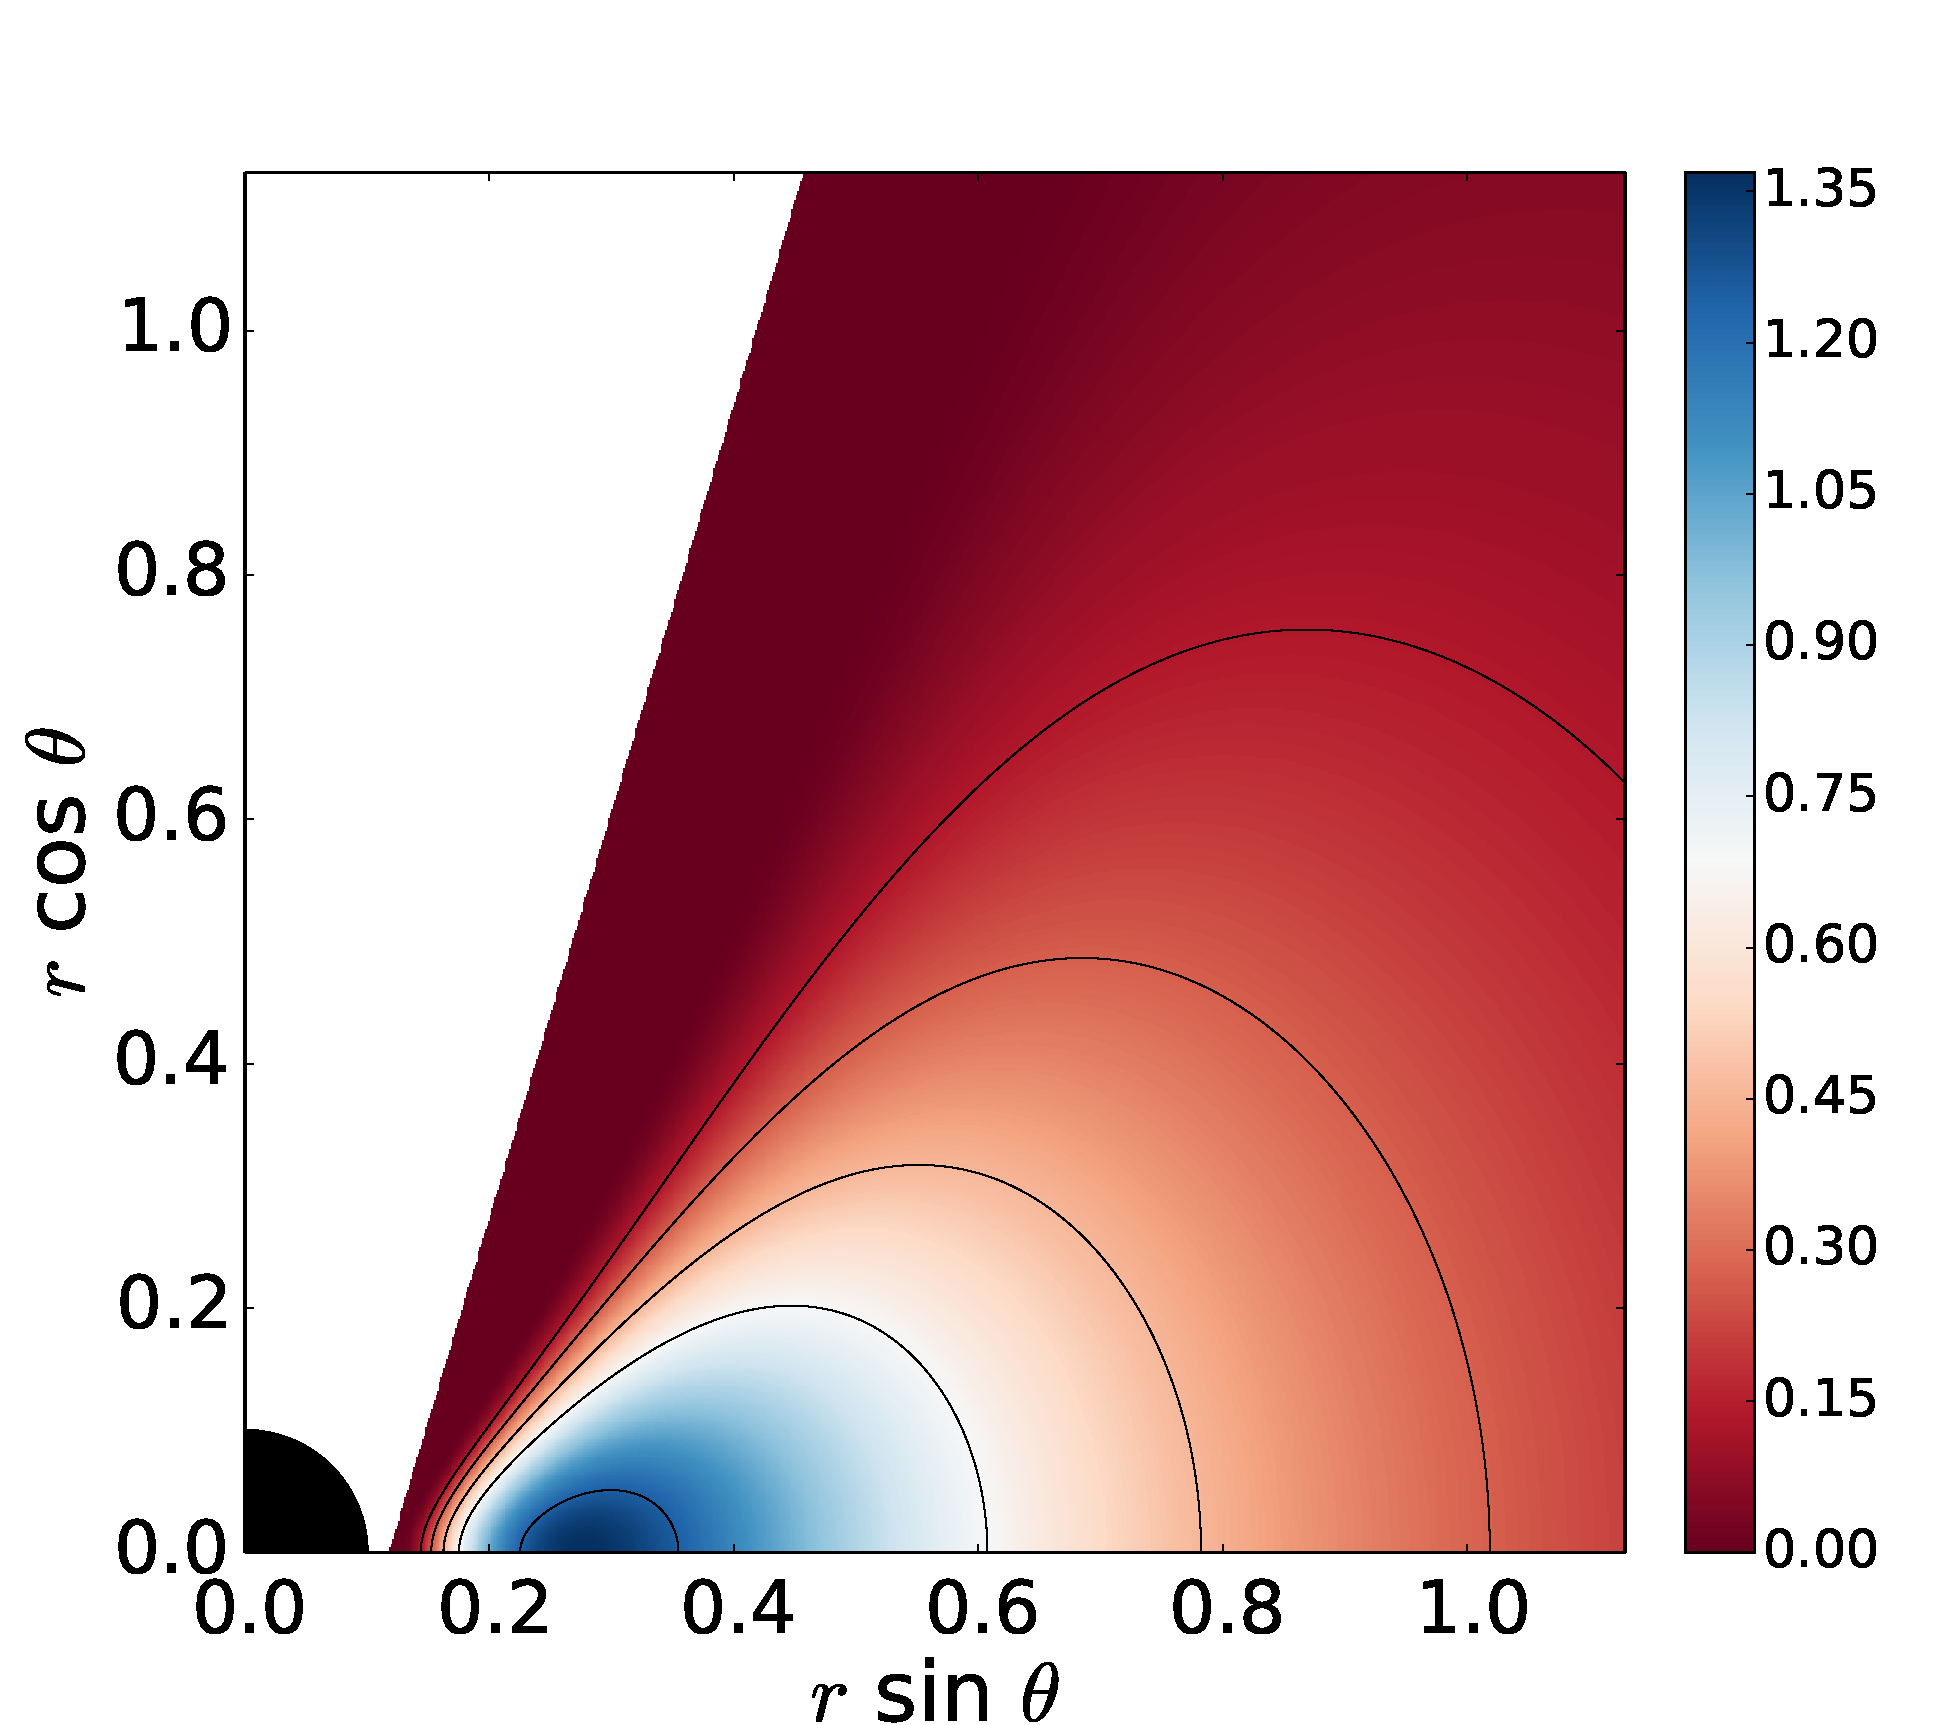
\includegraphics[scale=0.2]{figures/fig3_IV_HBH_0.pdf}
\hspace{-0.3cm}
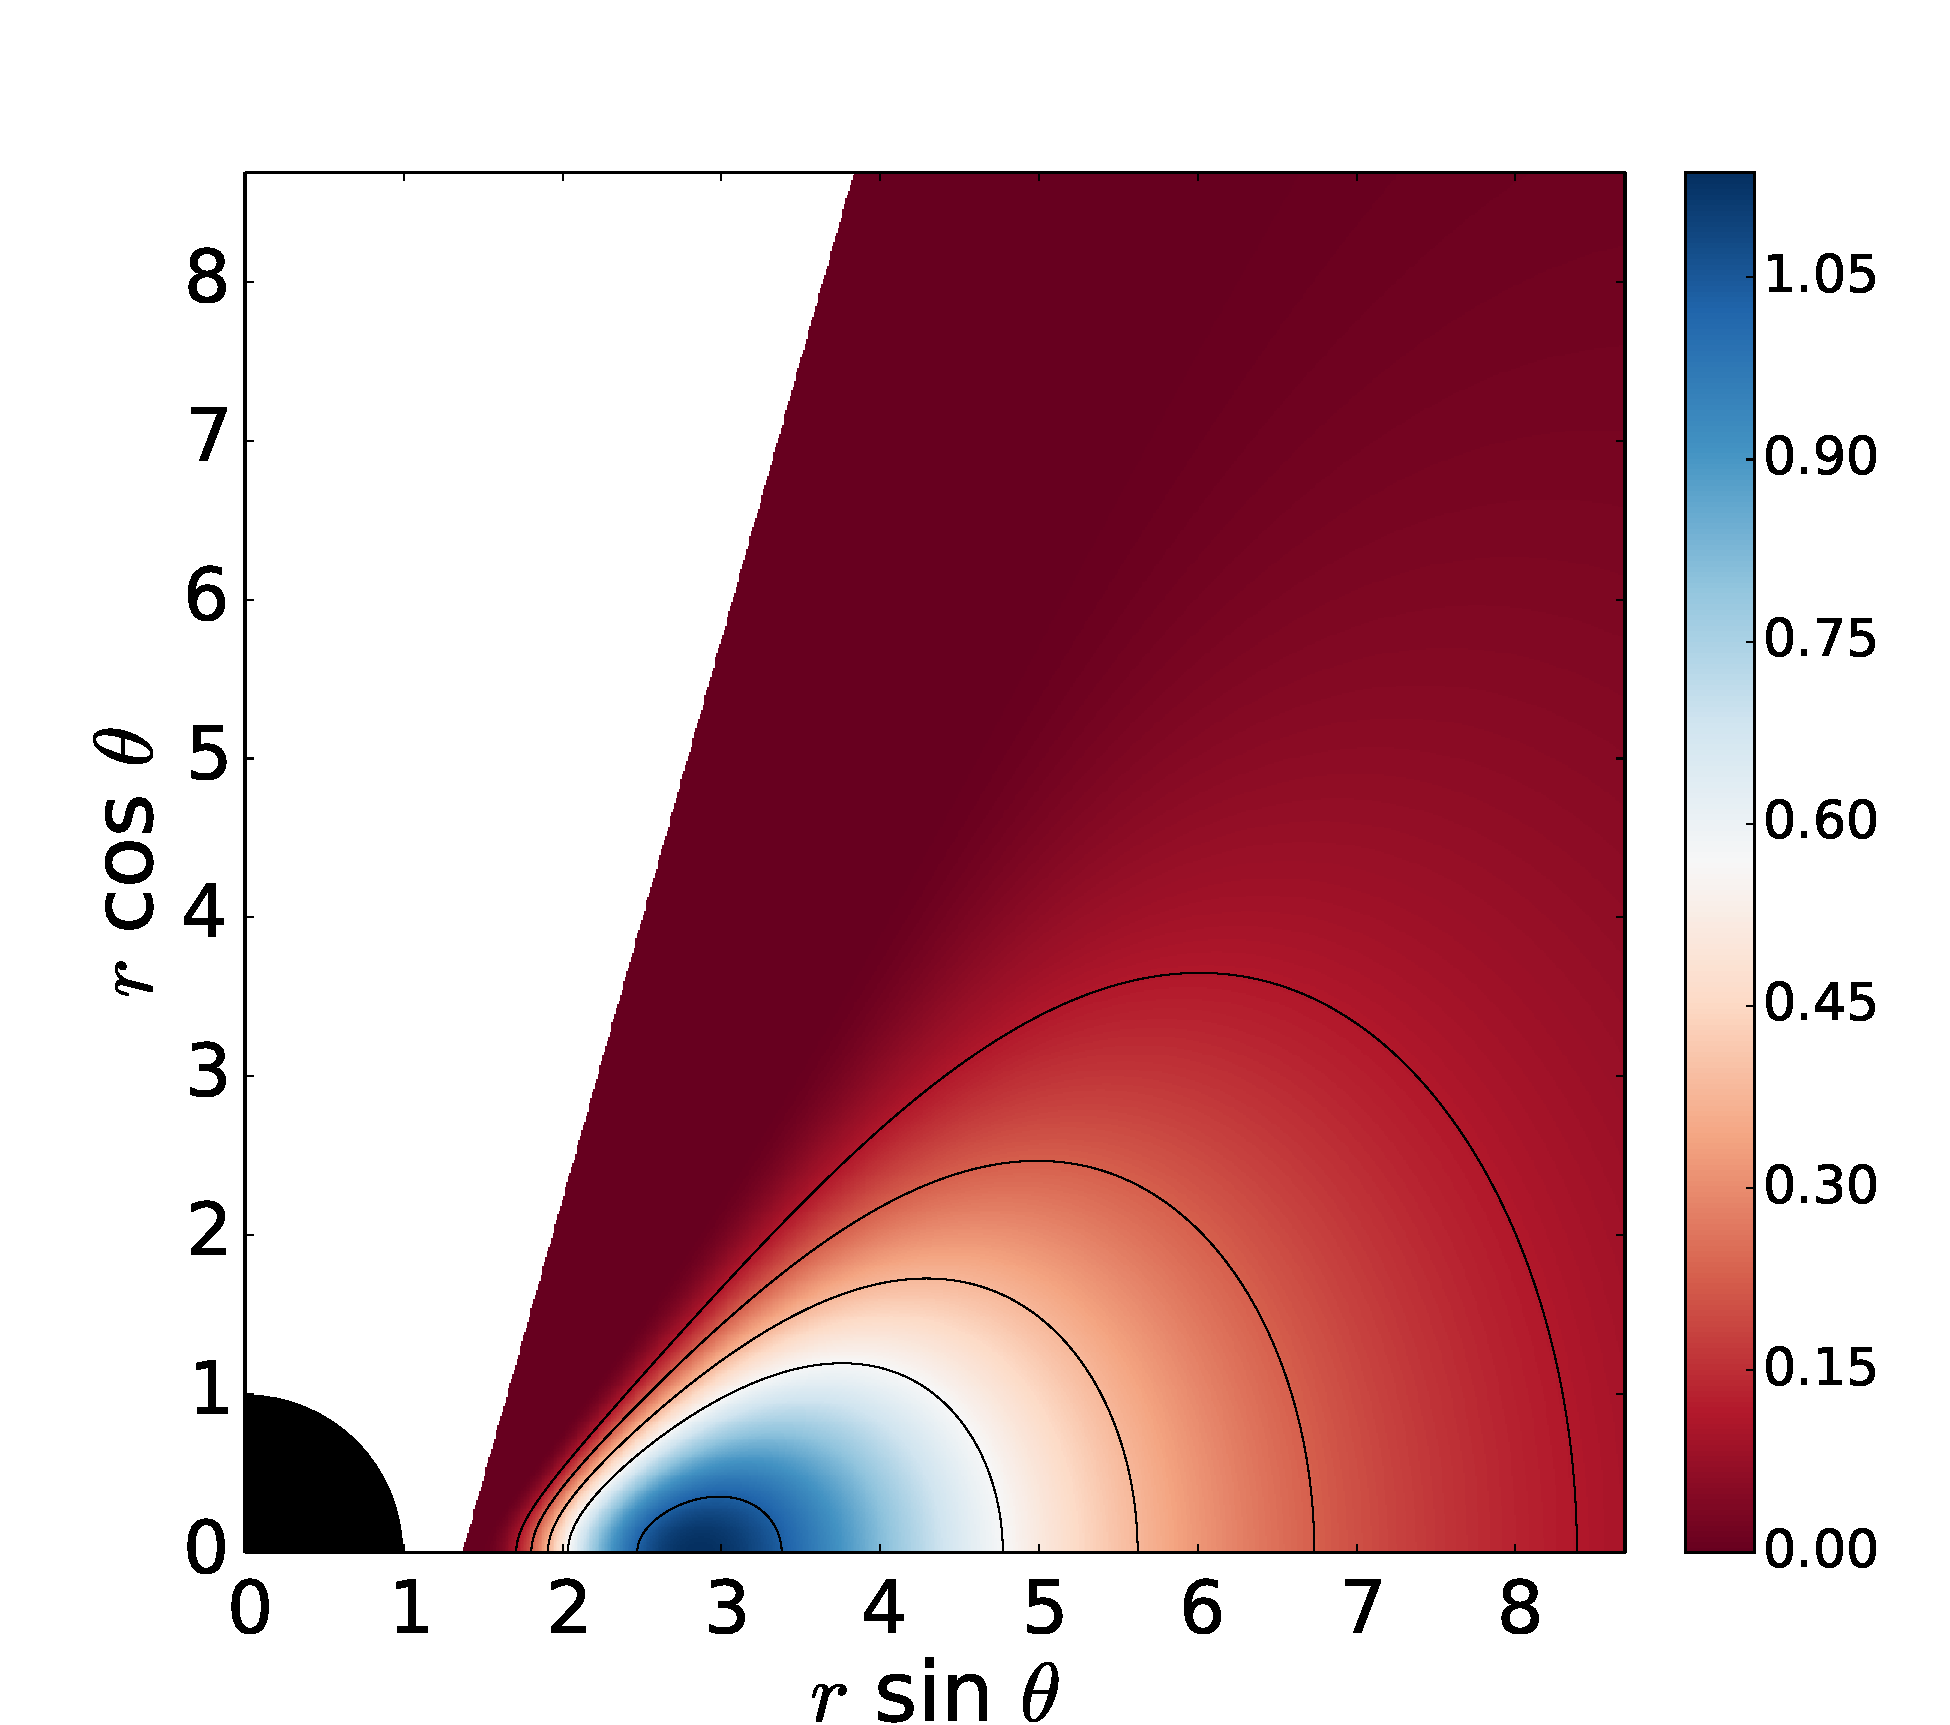
\includegraphics[scale=0.2]{figures/fig3_IV_ADM_0.pdf}
\hspace{-0.2cm}
\\
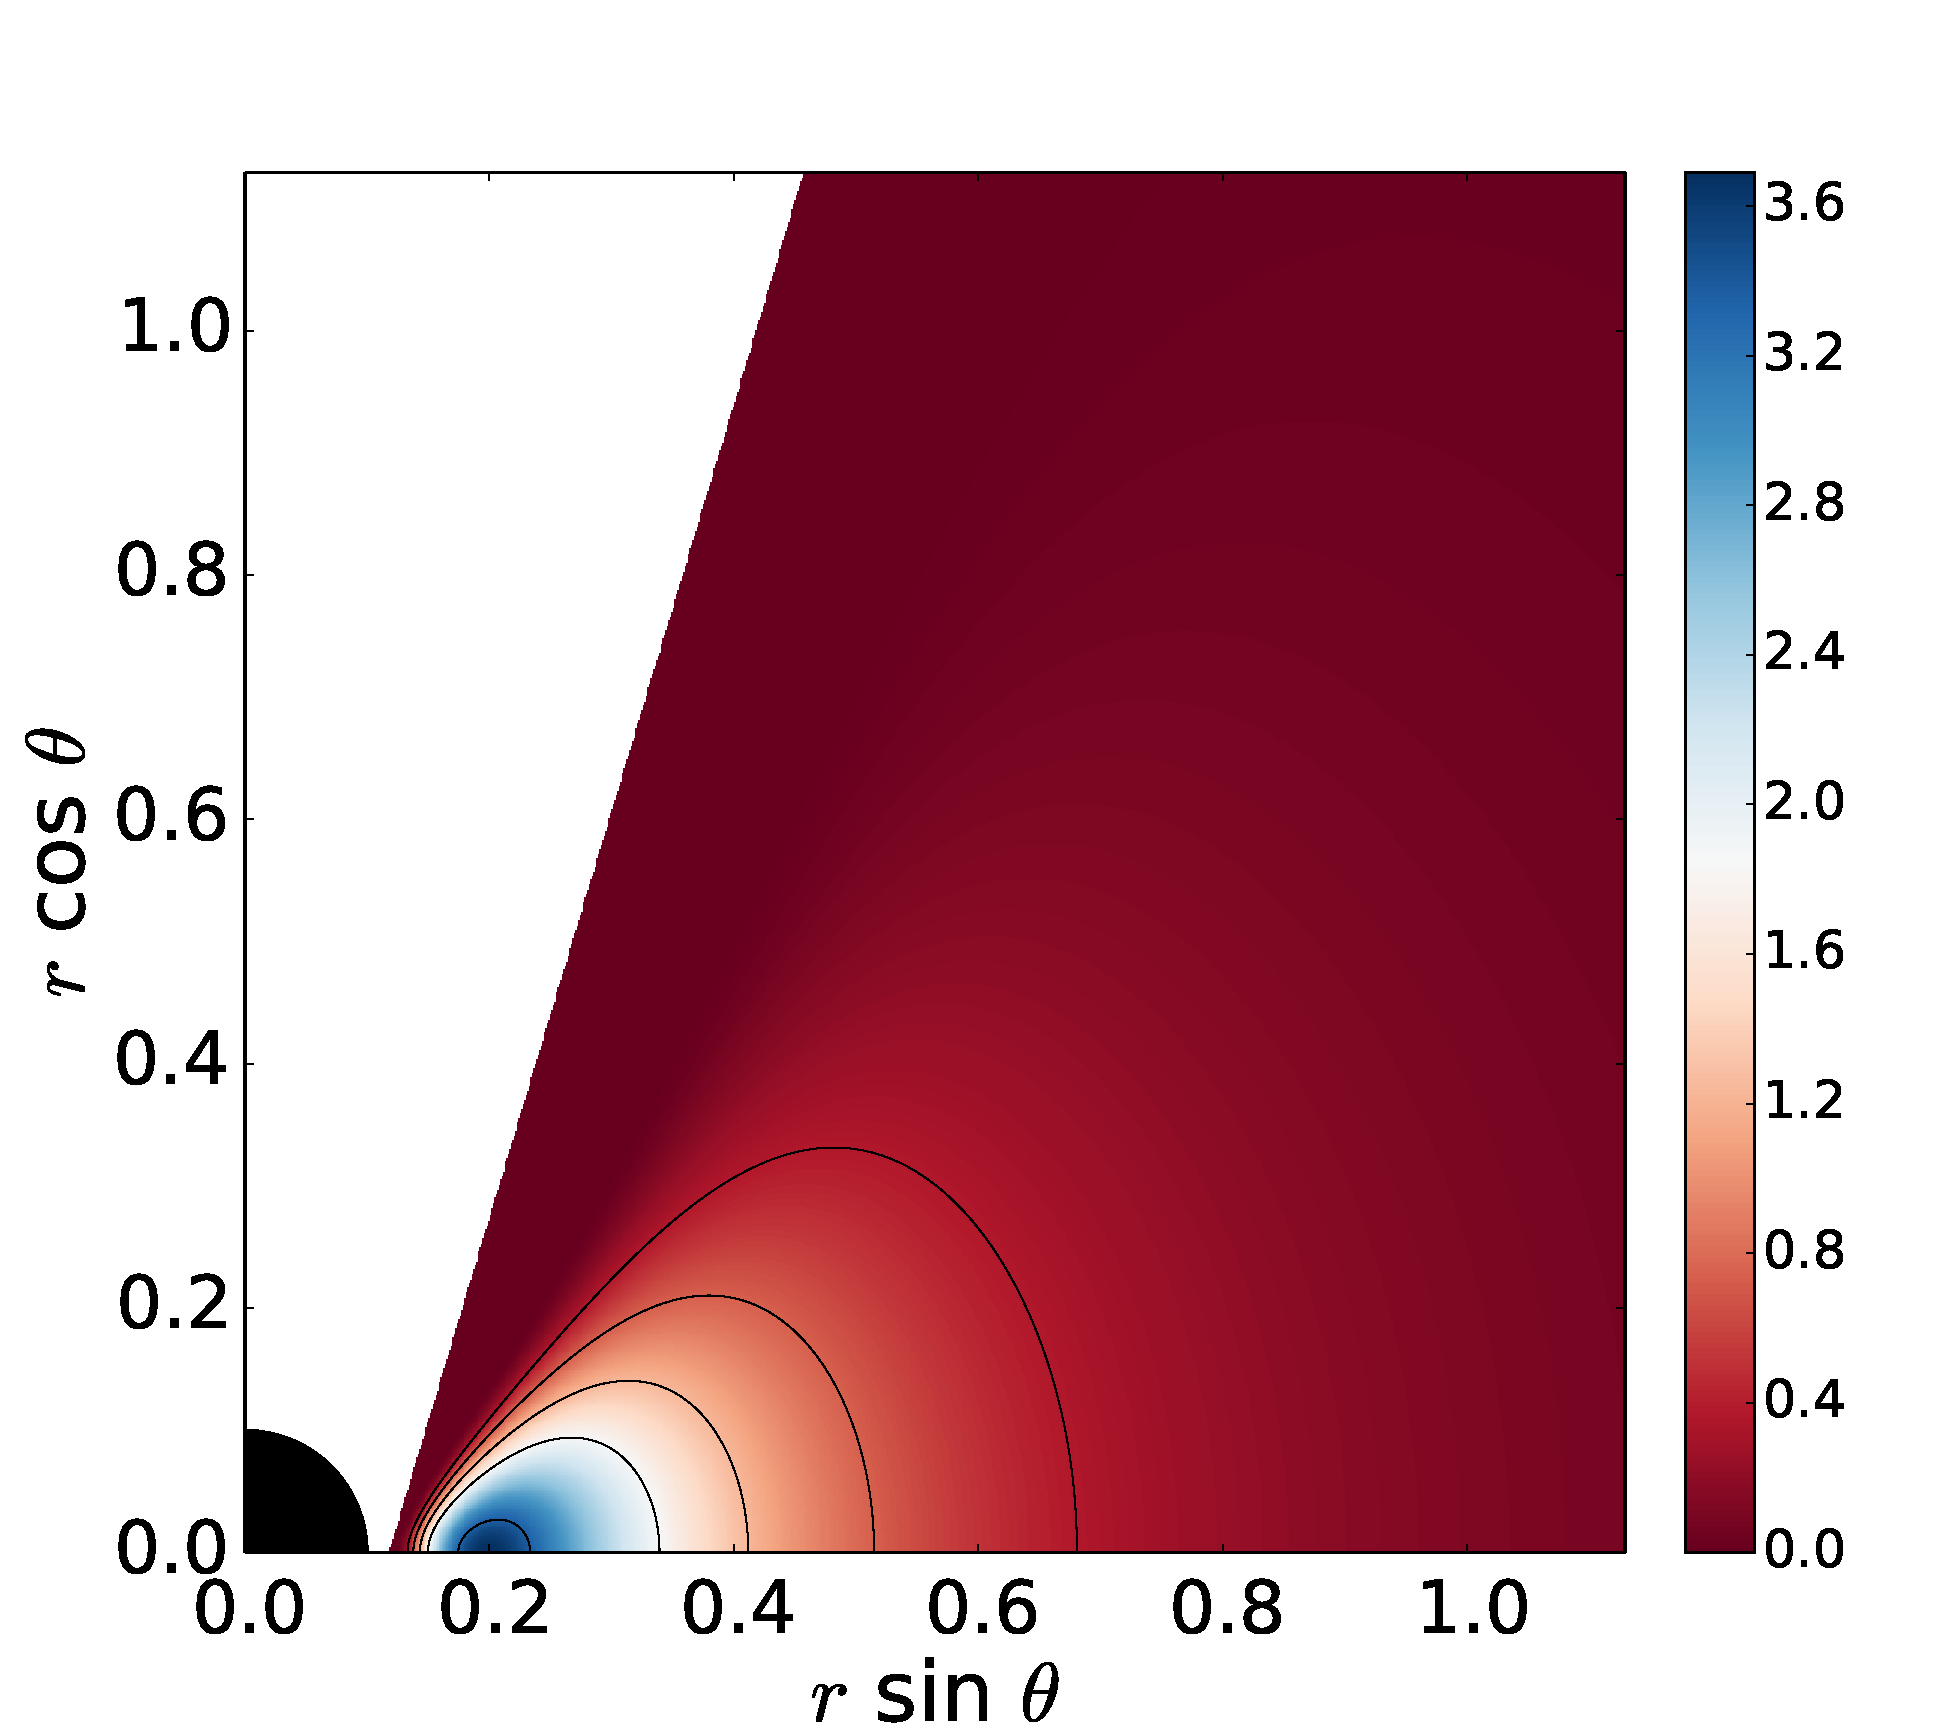
\includegraphics[scale=0.2]{figures/fig3_IV_HBH__3.pdf}
\hspace{-0.3cm}
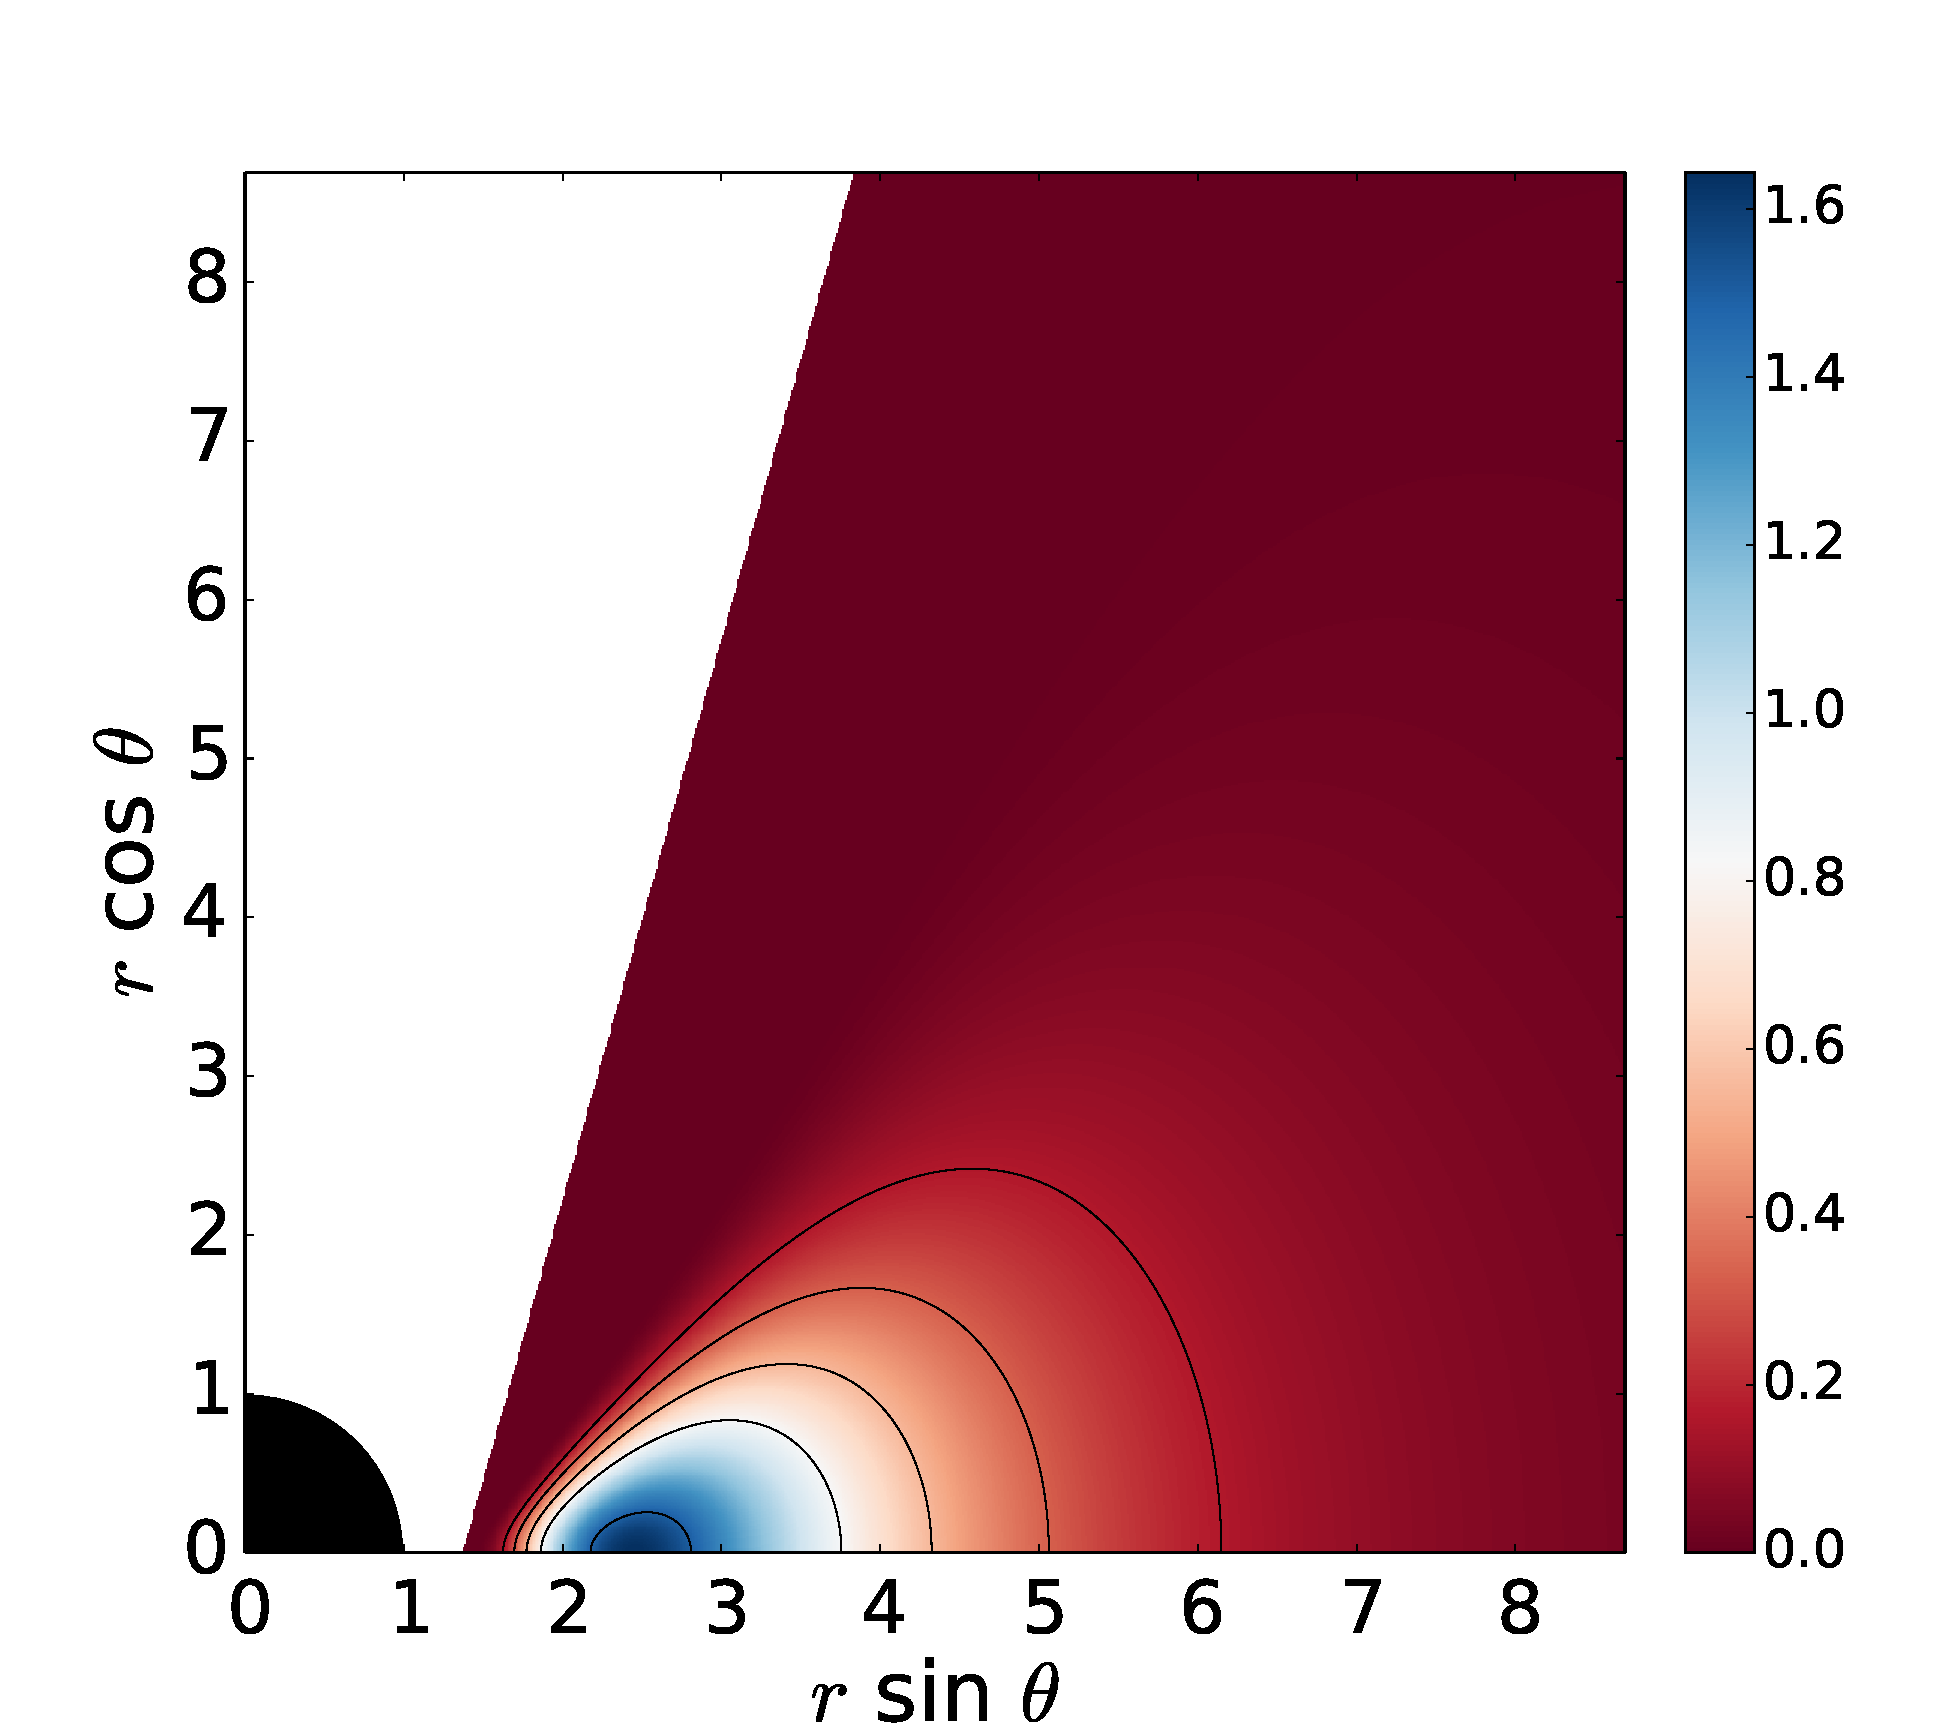
\includegraphics[scale=0.2]{figures/fig3_IV_ADM__3.pdf}
\hspace{-0.2cm}
\caption{Rest-mass density distribution for the model II. From top to bottom the rows correspond to the different values of the magnetization parameter, namely non-magnetized ($\beta_{\mathrm{m}_{\mathrm{c}}} = 10^{3}$), mildly magnetized ($\beta_{\mathrm{m}_{\mathrm{c}}} = 1$) and strongly magnetized ($\beta_{\mathrm{m}_{\mathrm{c}}} = 10^{-3}$). The left column correspond to the KBHsSH model and the right column correspond to the corresponding KBH with the same ADM quantities.}
\label{comparison_mag_2}
\end{figure*}

\begin{figure*}
\centering
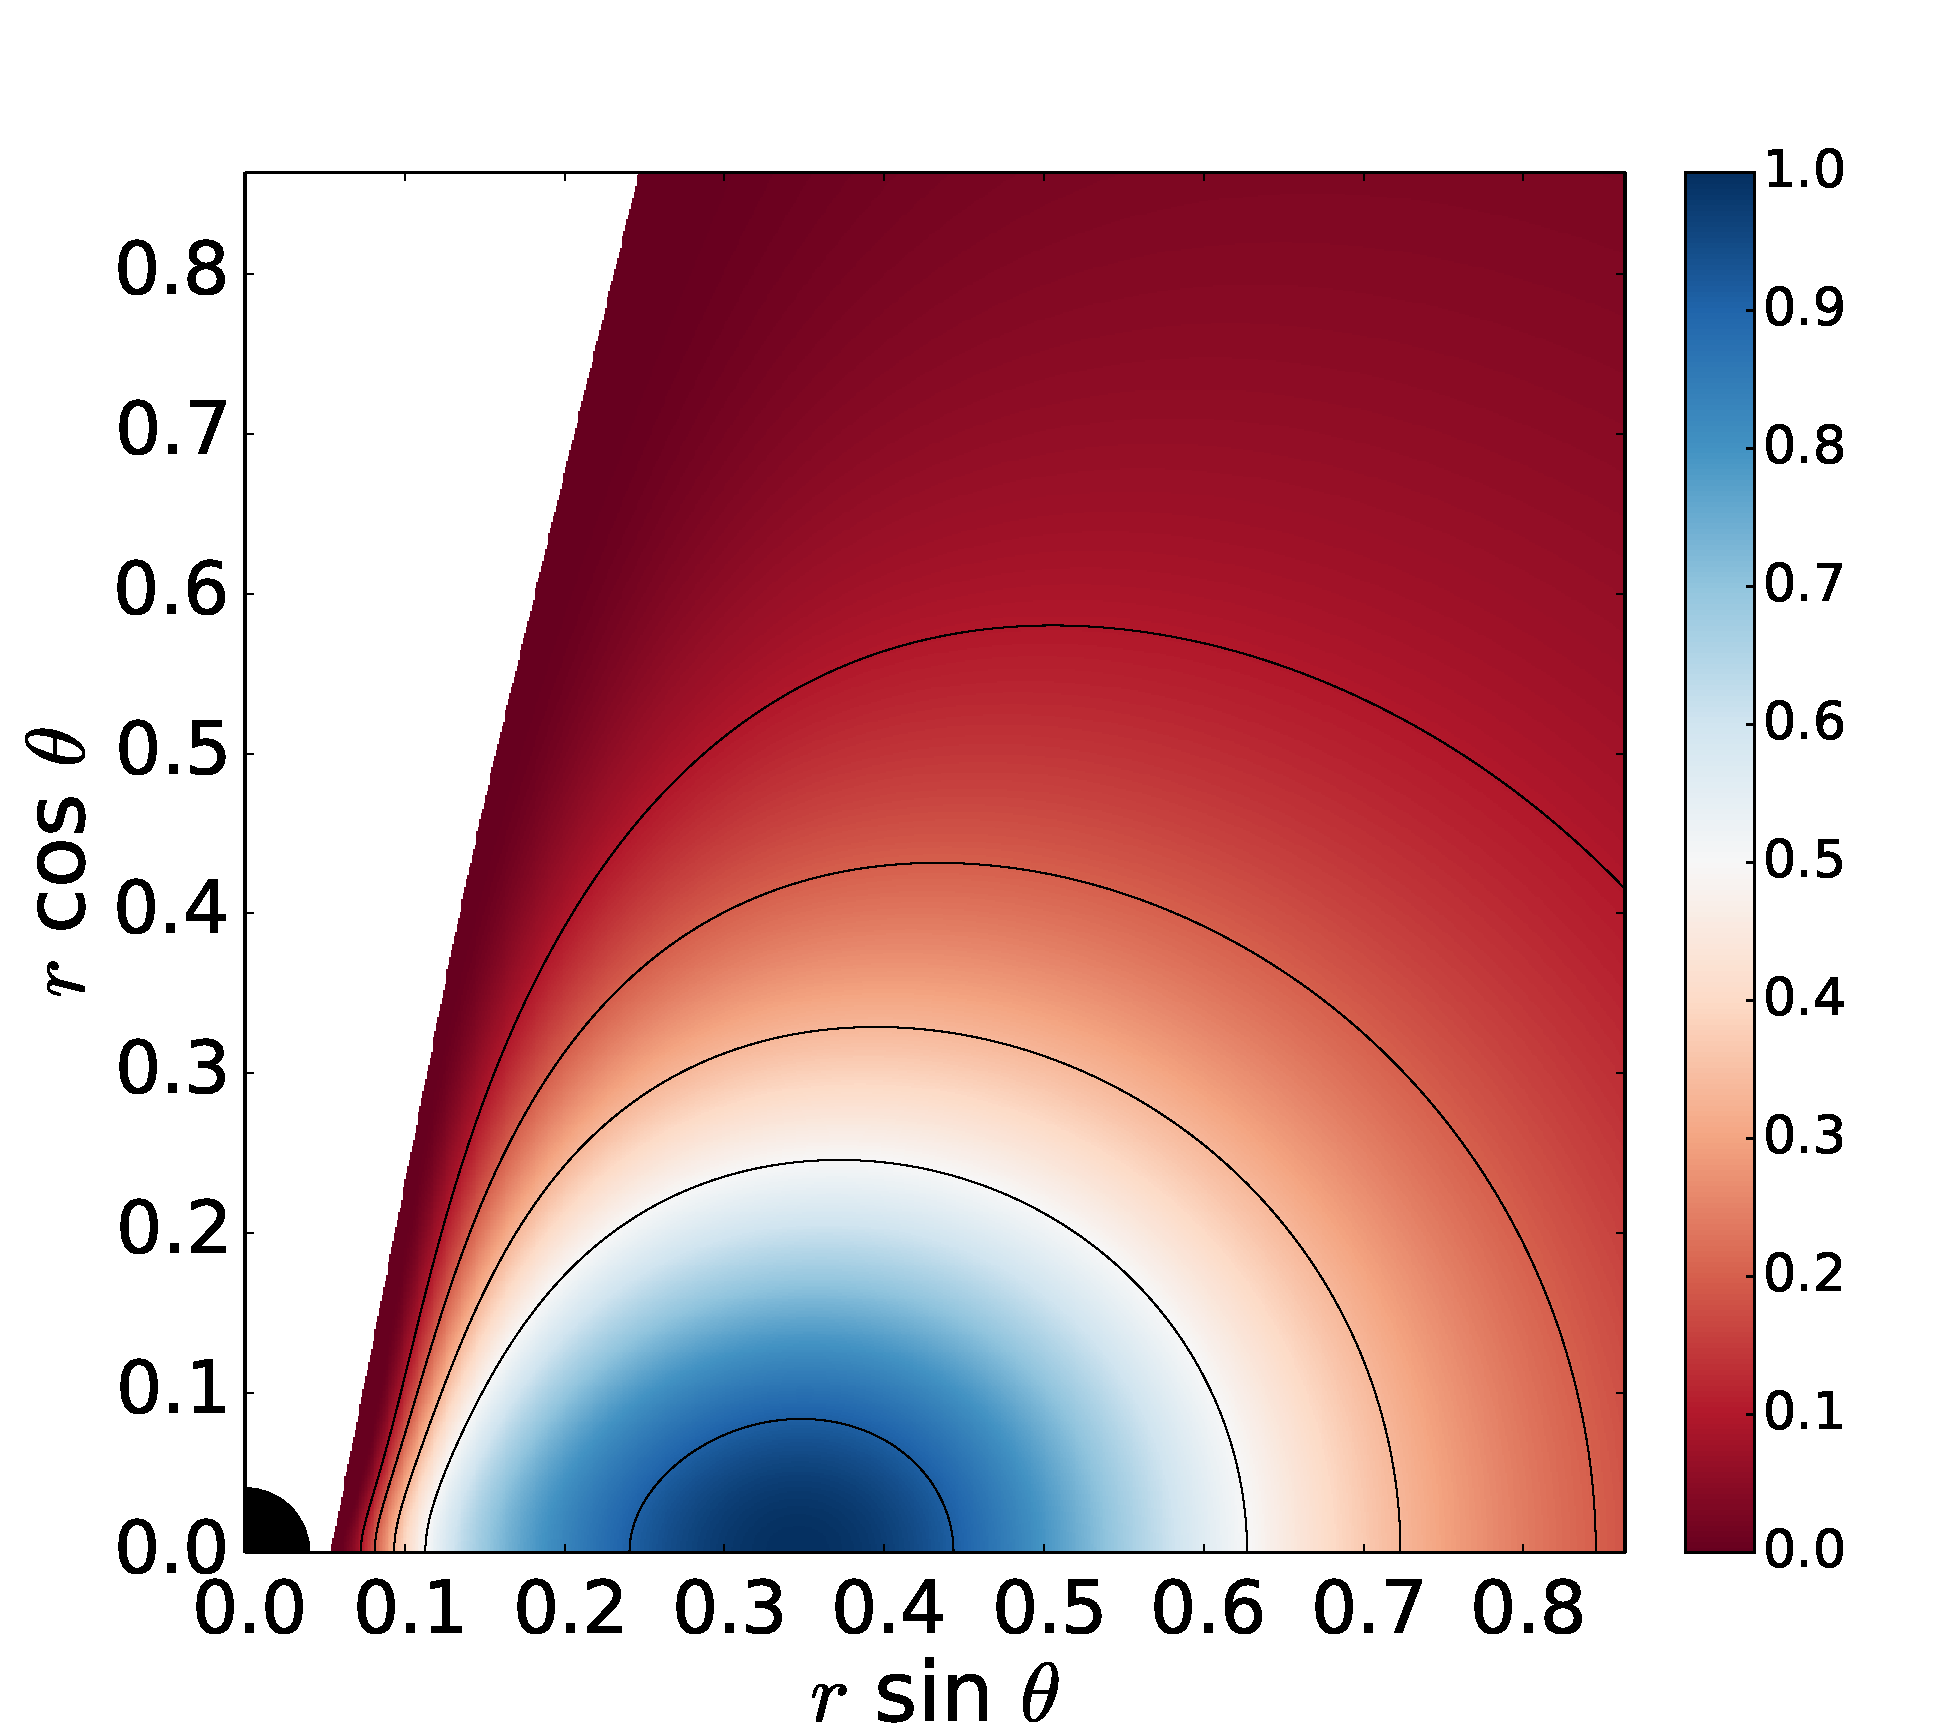
\includegraphics[scale=0.2]{figures/fig4_V_HBH_3.pdf}
\hspace{-0.3cm}
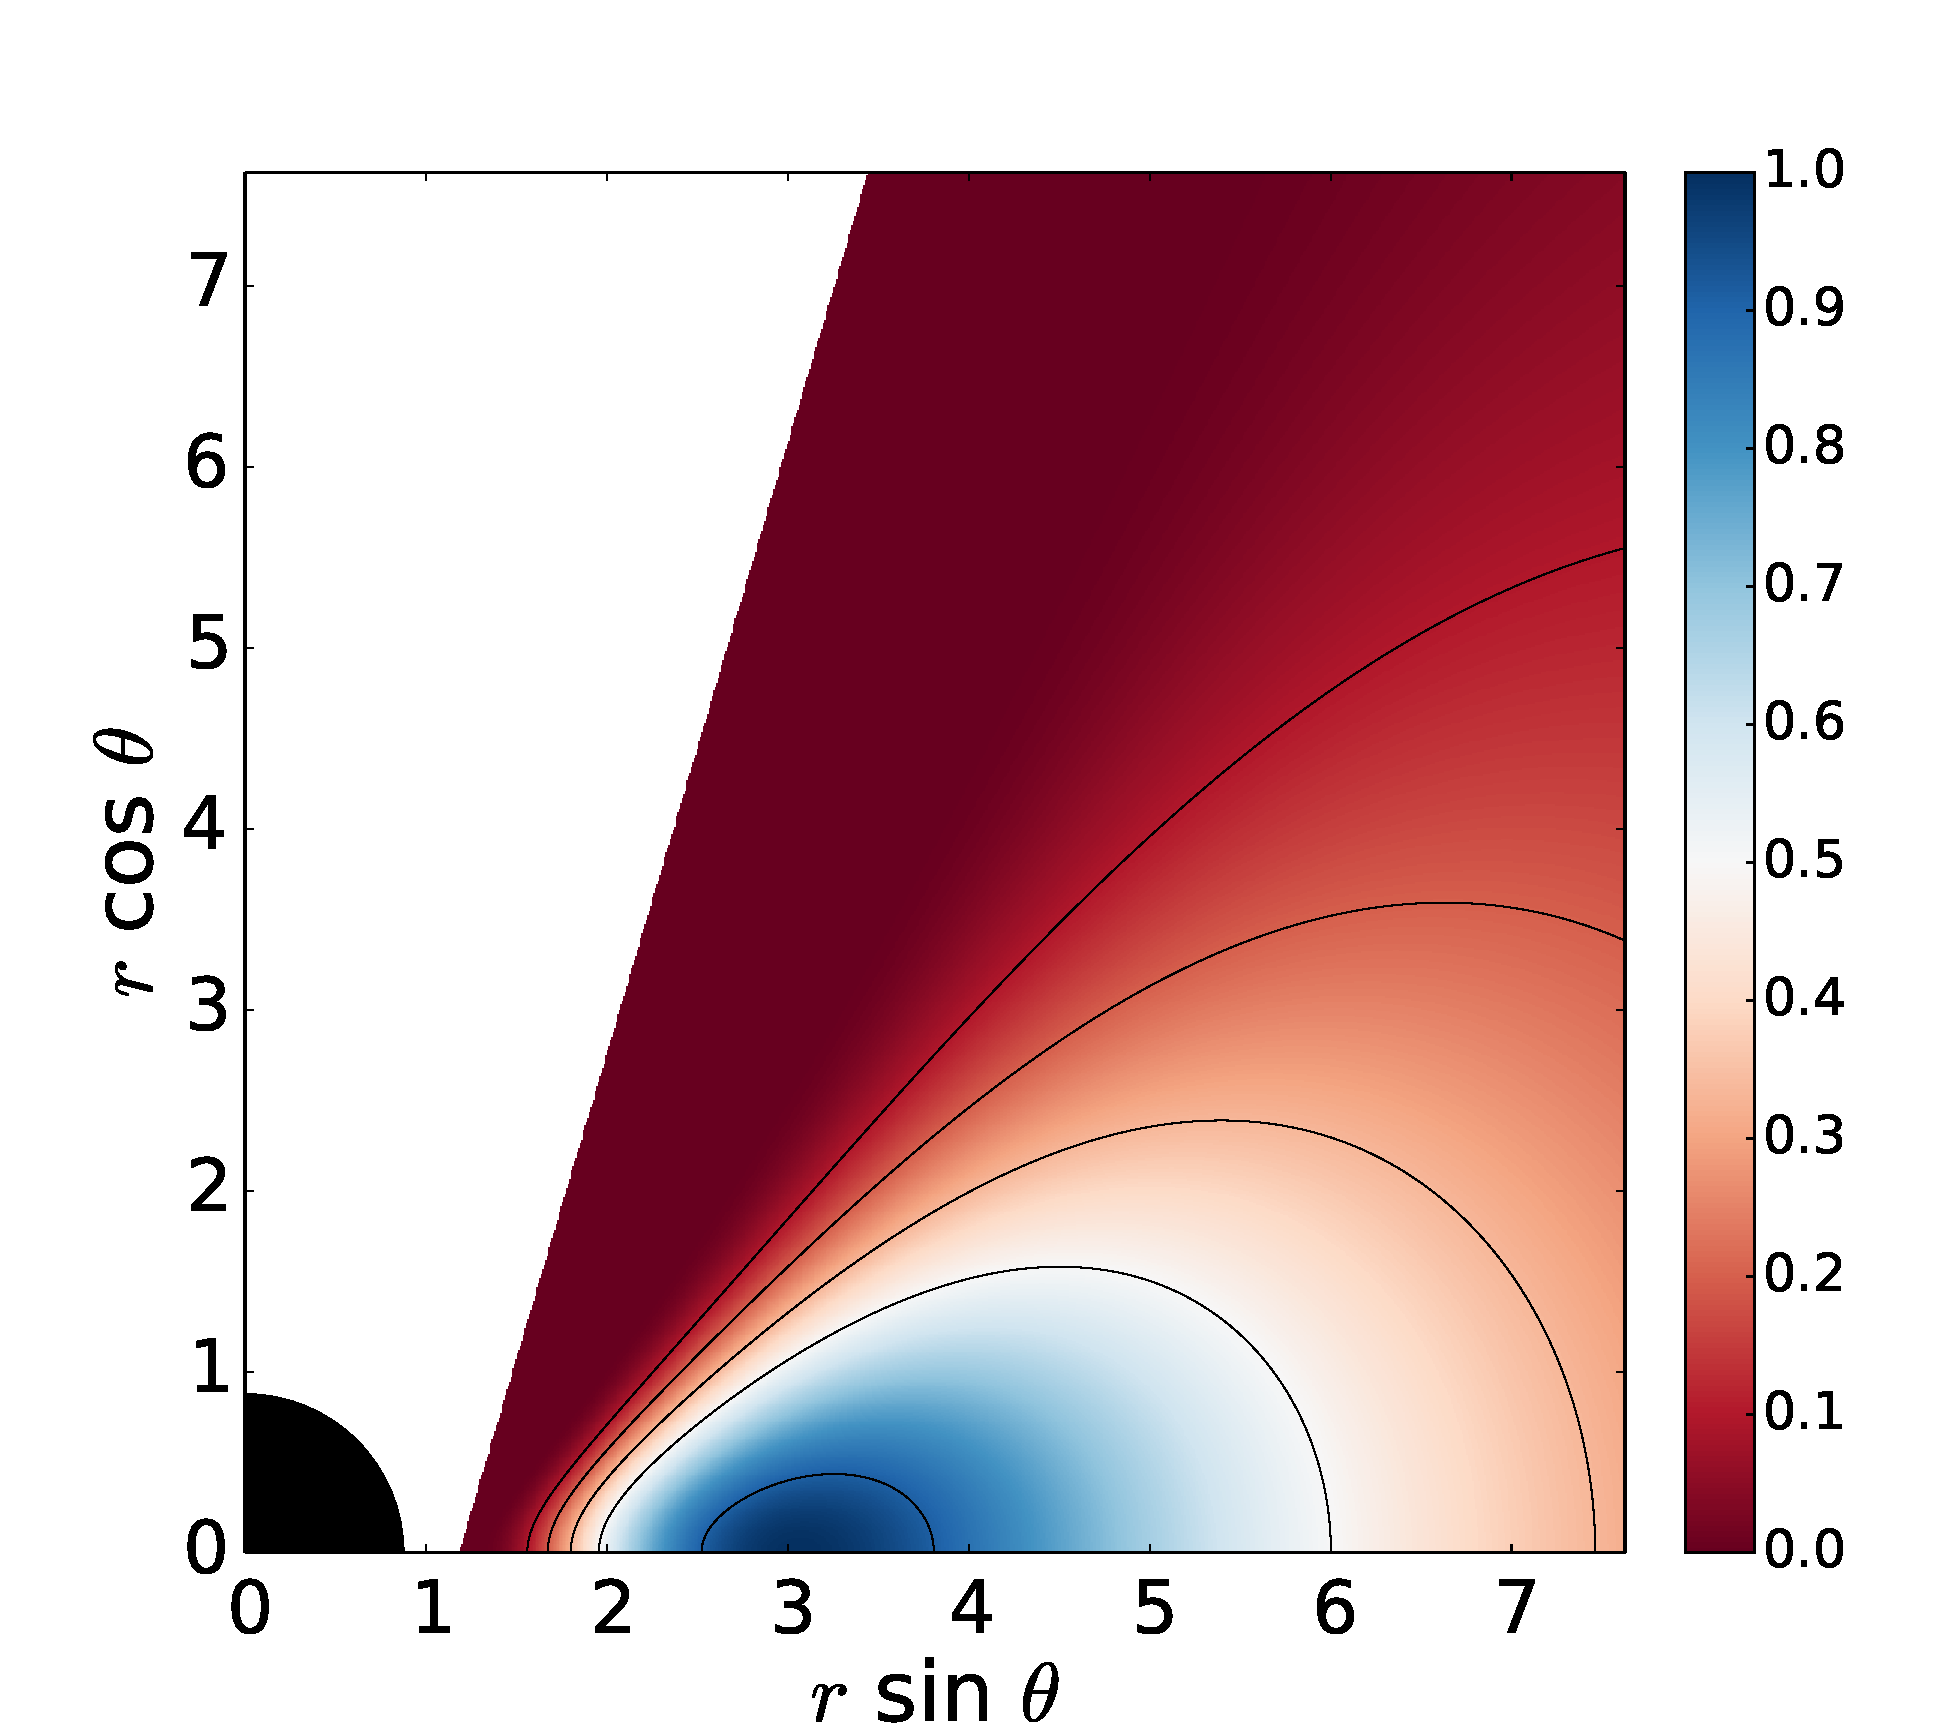
\includegraphics[scale=0.2]{figures/fig4_V_ADM_3.pdf}
\hspace{-0.2cm}
\\
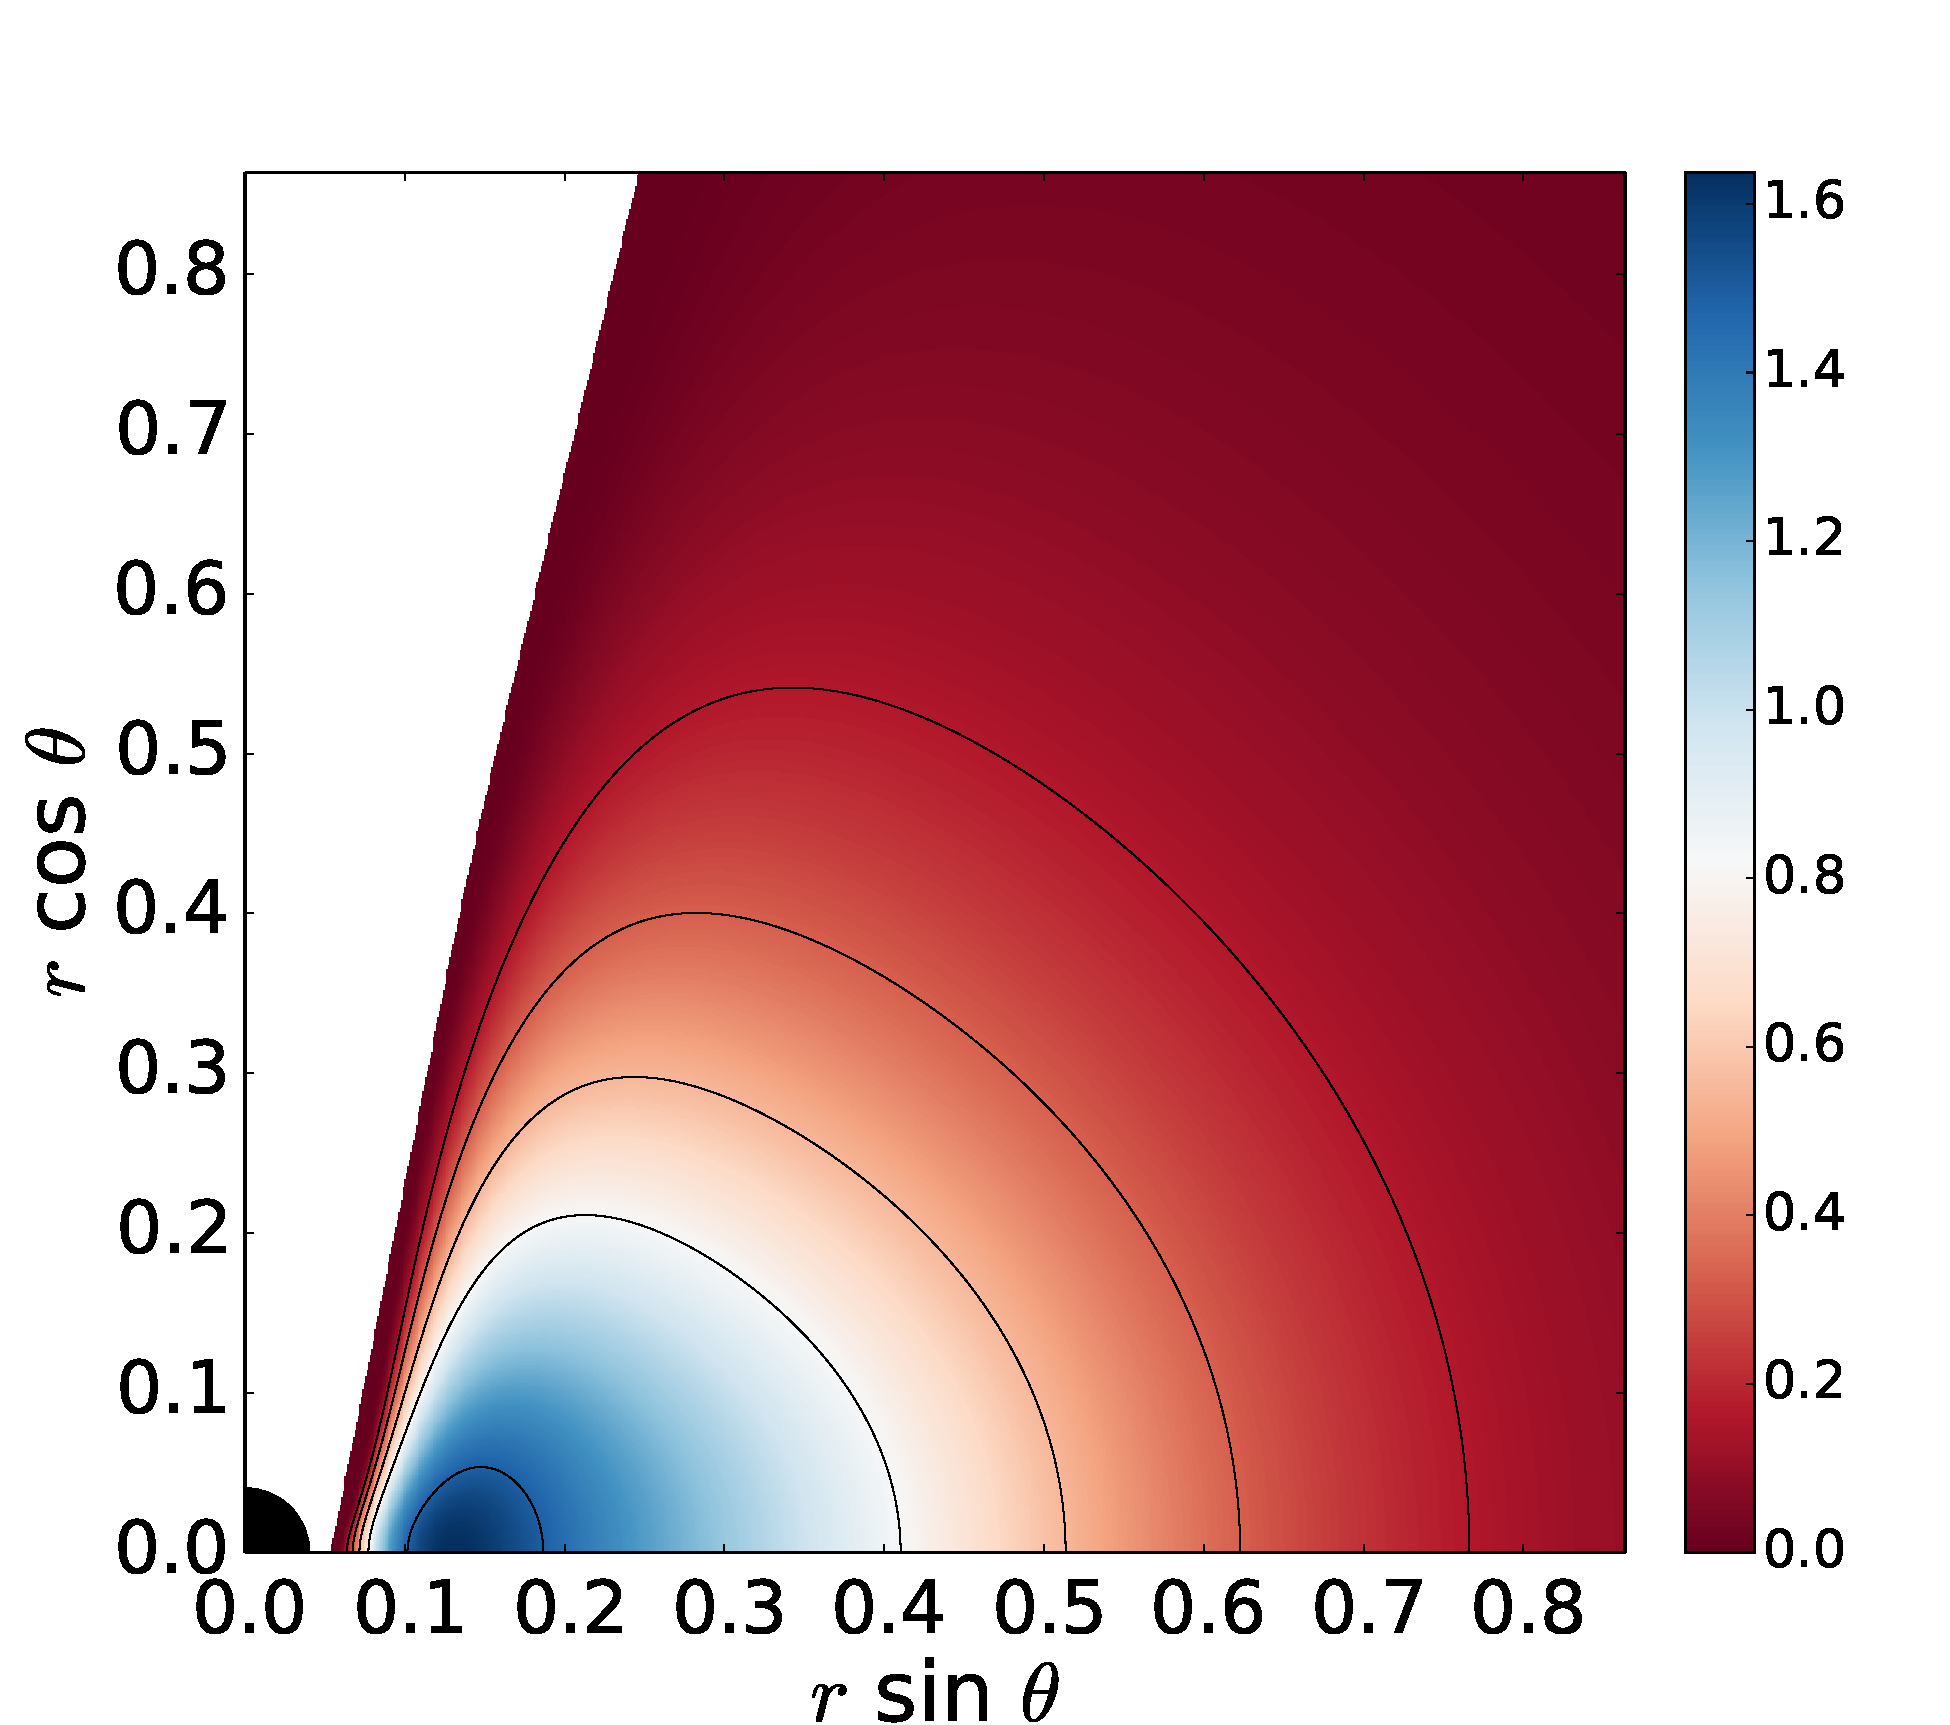
\includegraphics[scale=0.2]{figures/fig4_V_HBH_0.pdf}
\hspace{-0.3cm}
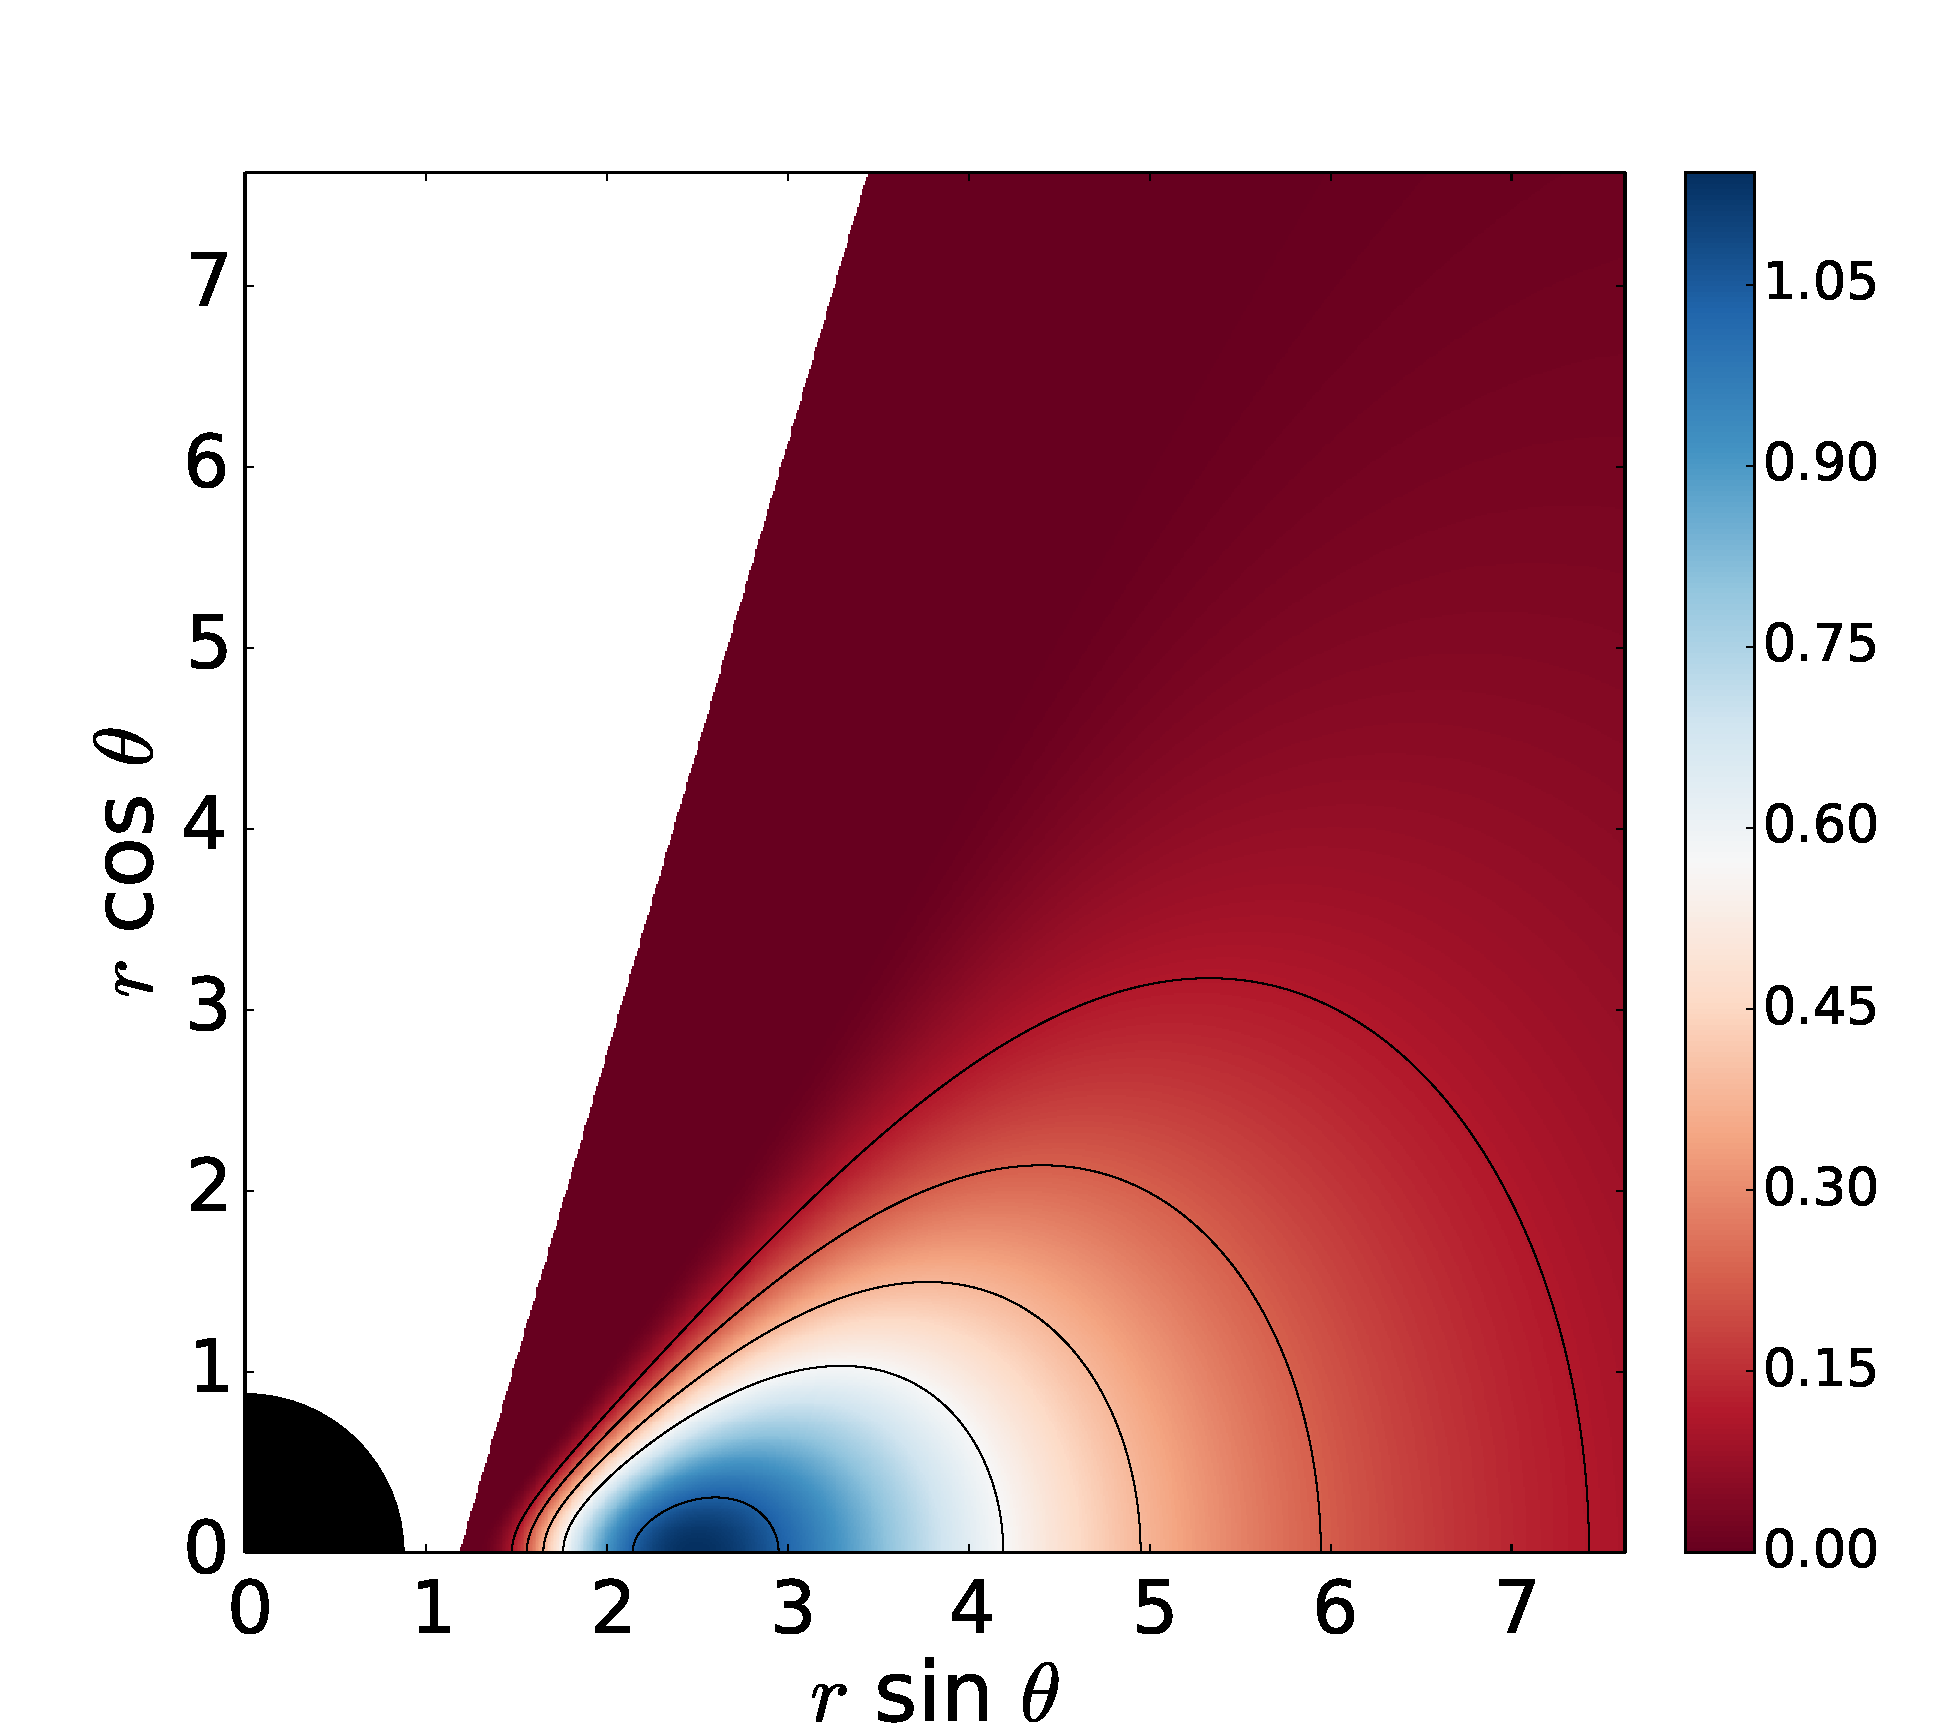
\includegraphics[scale=0.2]{figures/fig4_V_ADM_0.pdf}
\hspace{-0.2cm}
\\
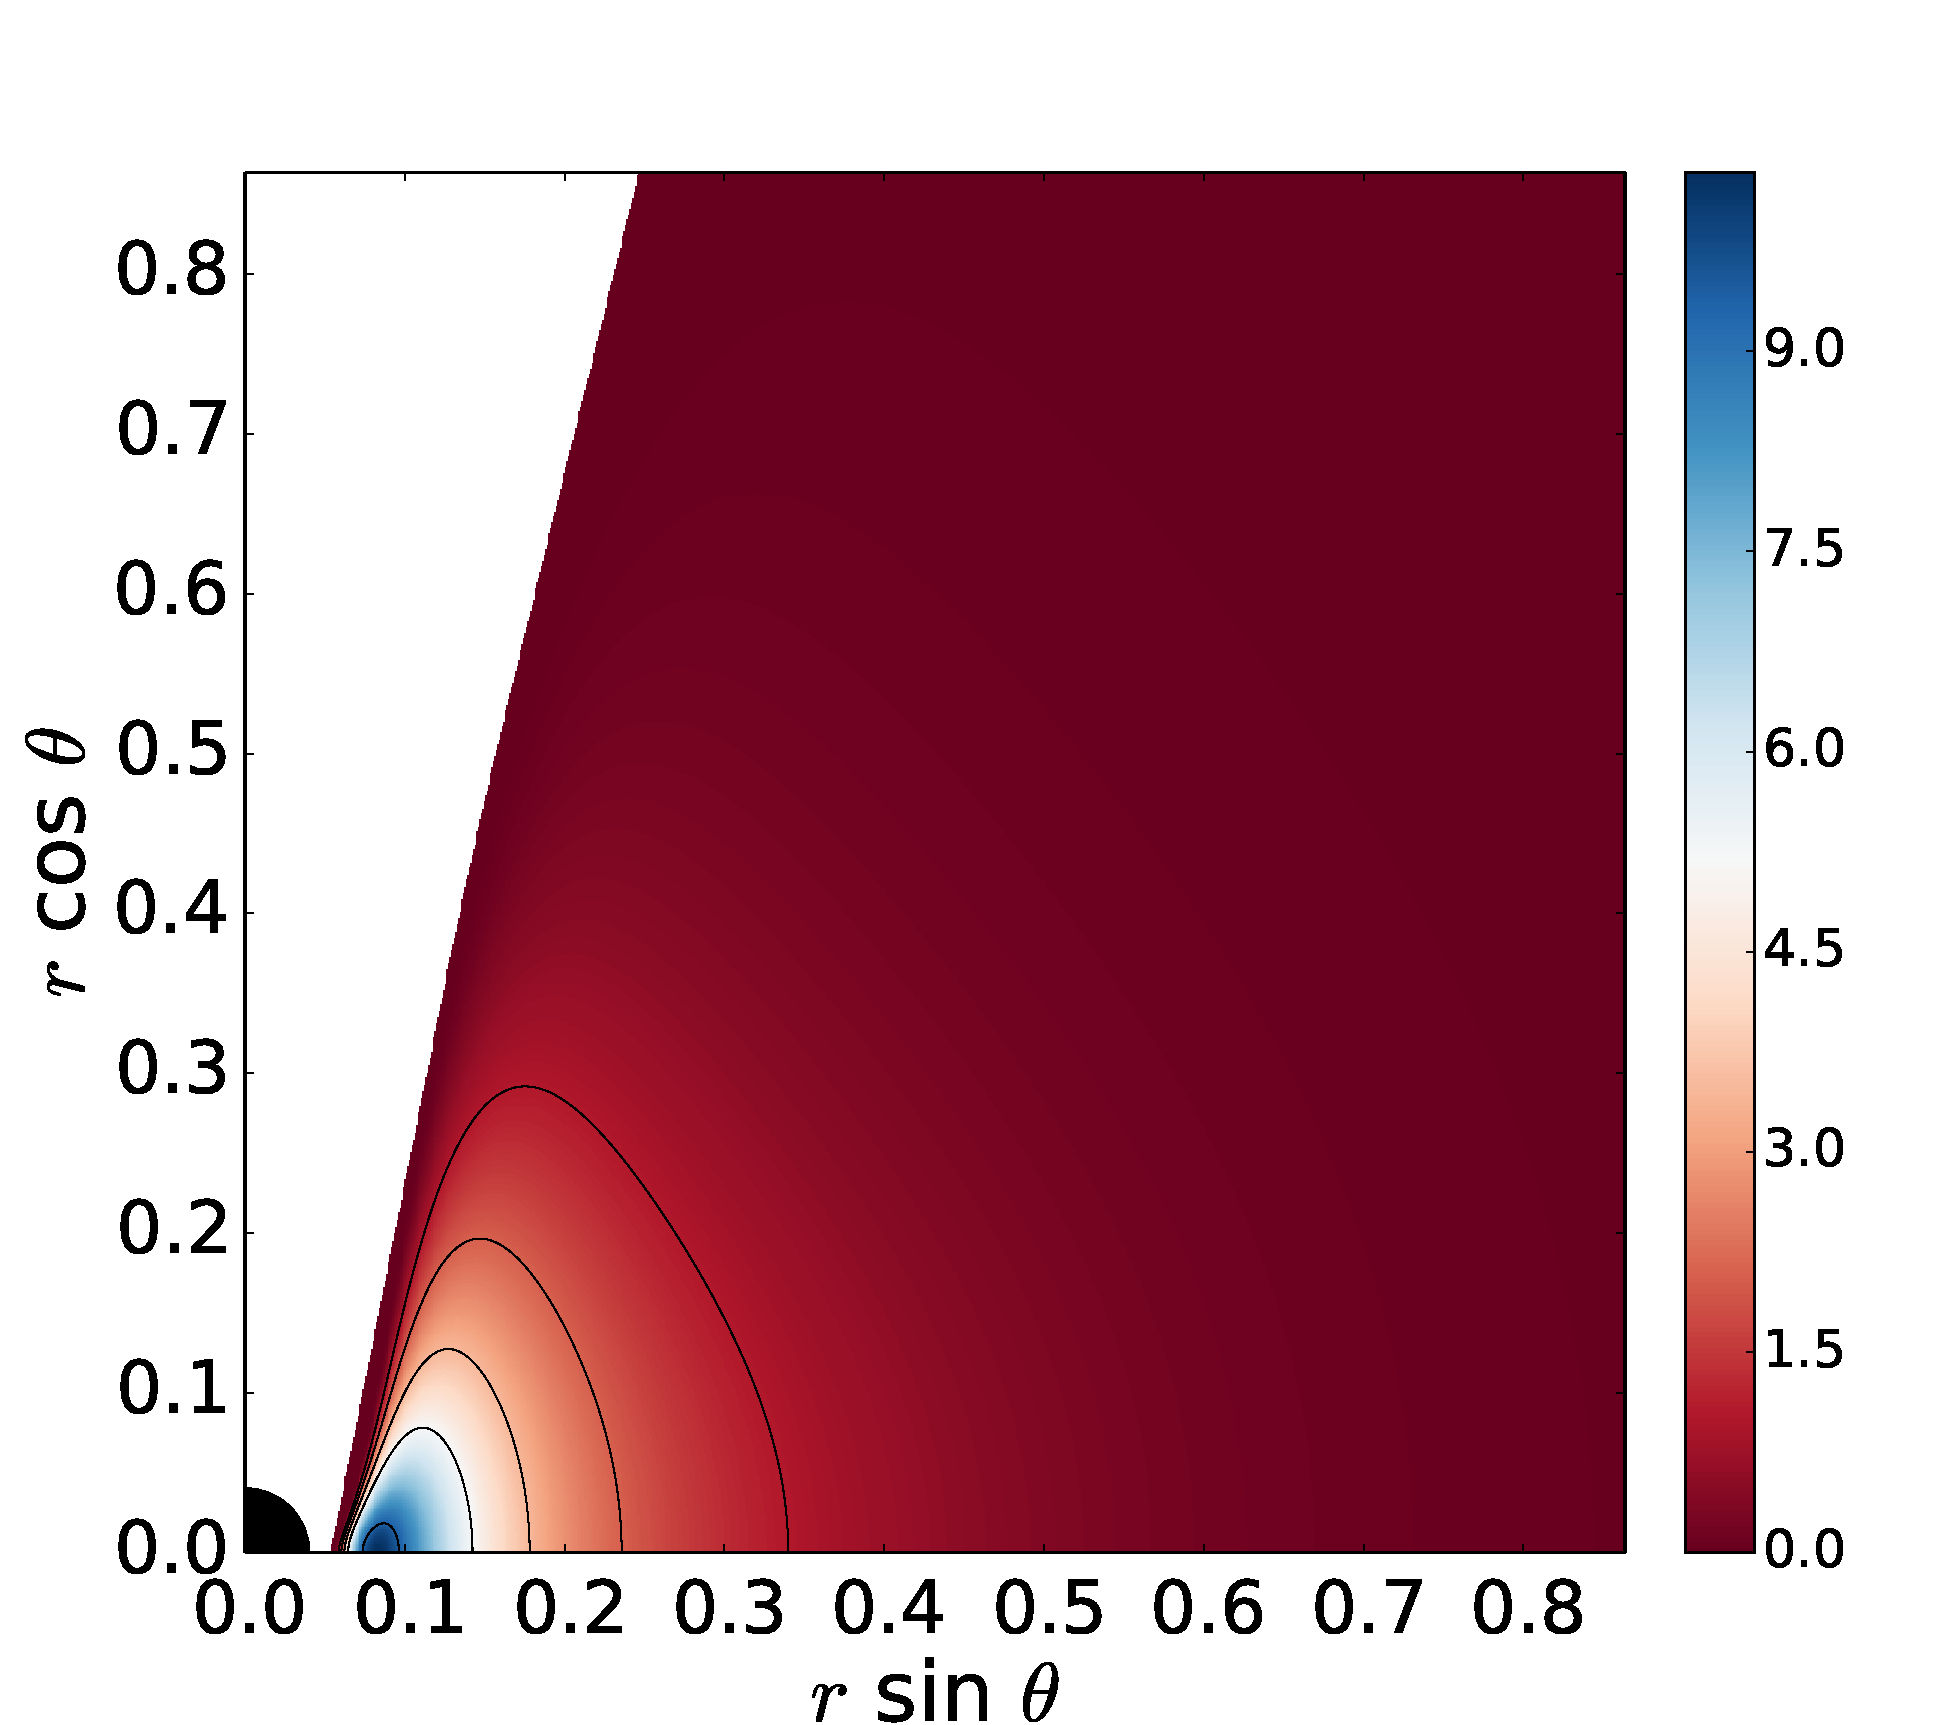
\includegraphics[scale=0.2]{figures/fig4_V_HBH__3.pdf}
\hspace{-0.3cm}
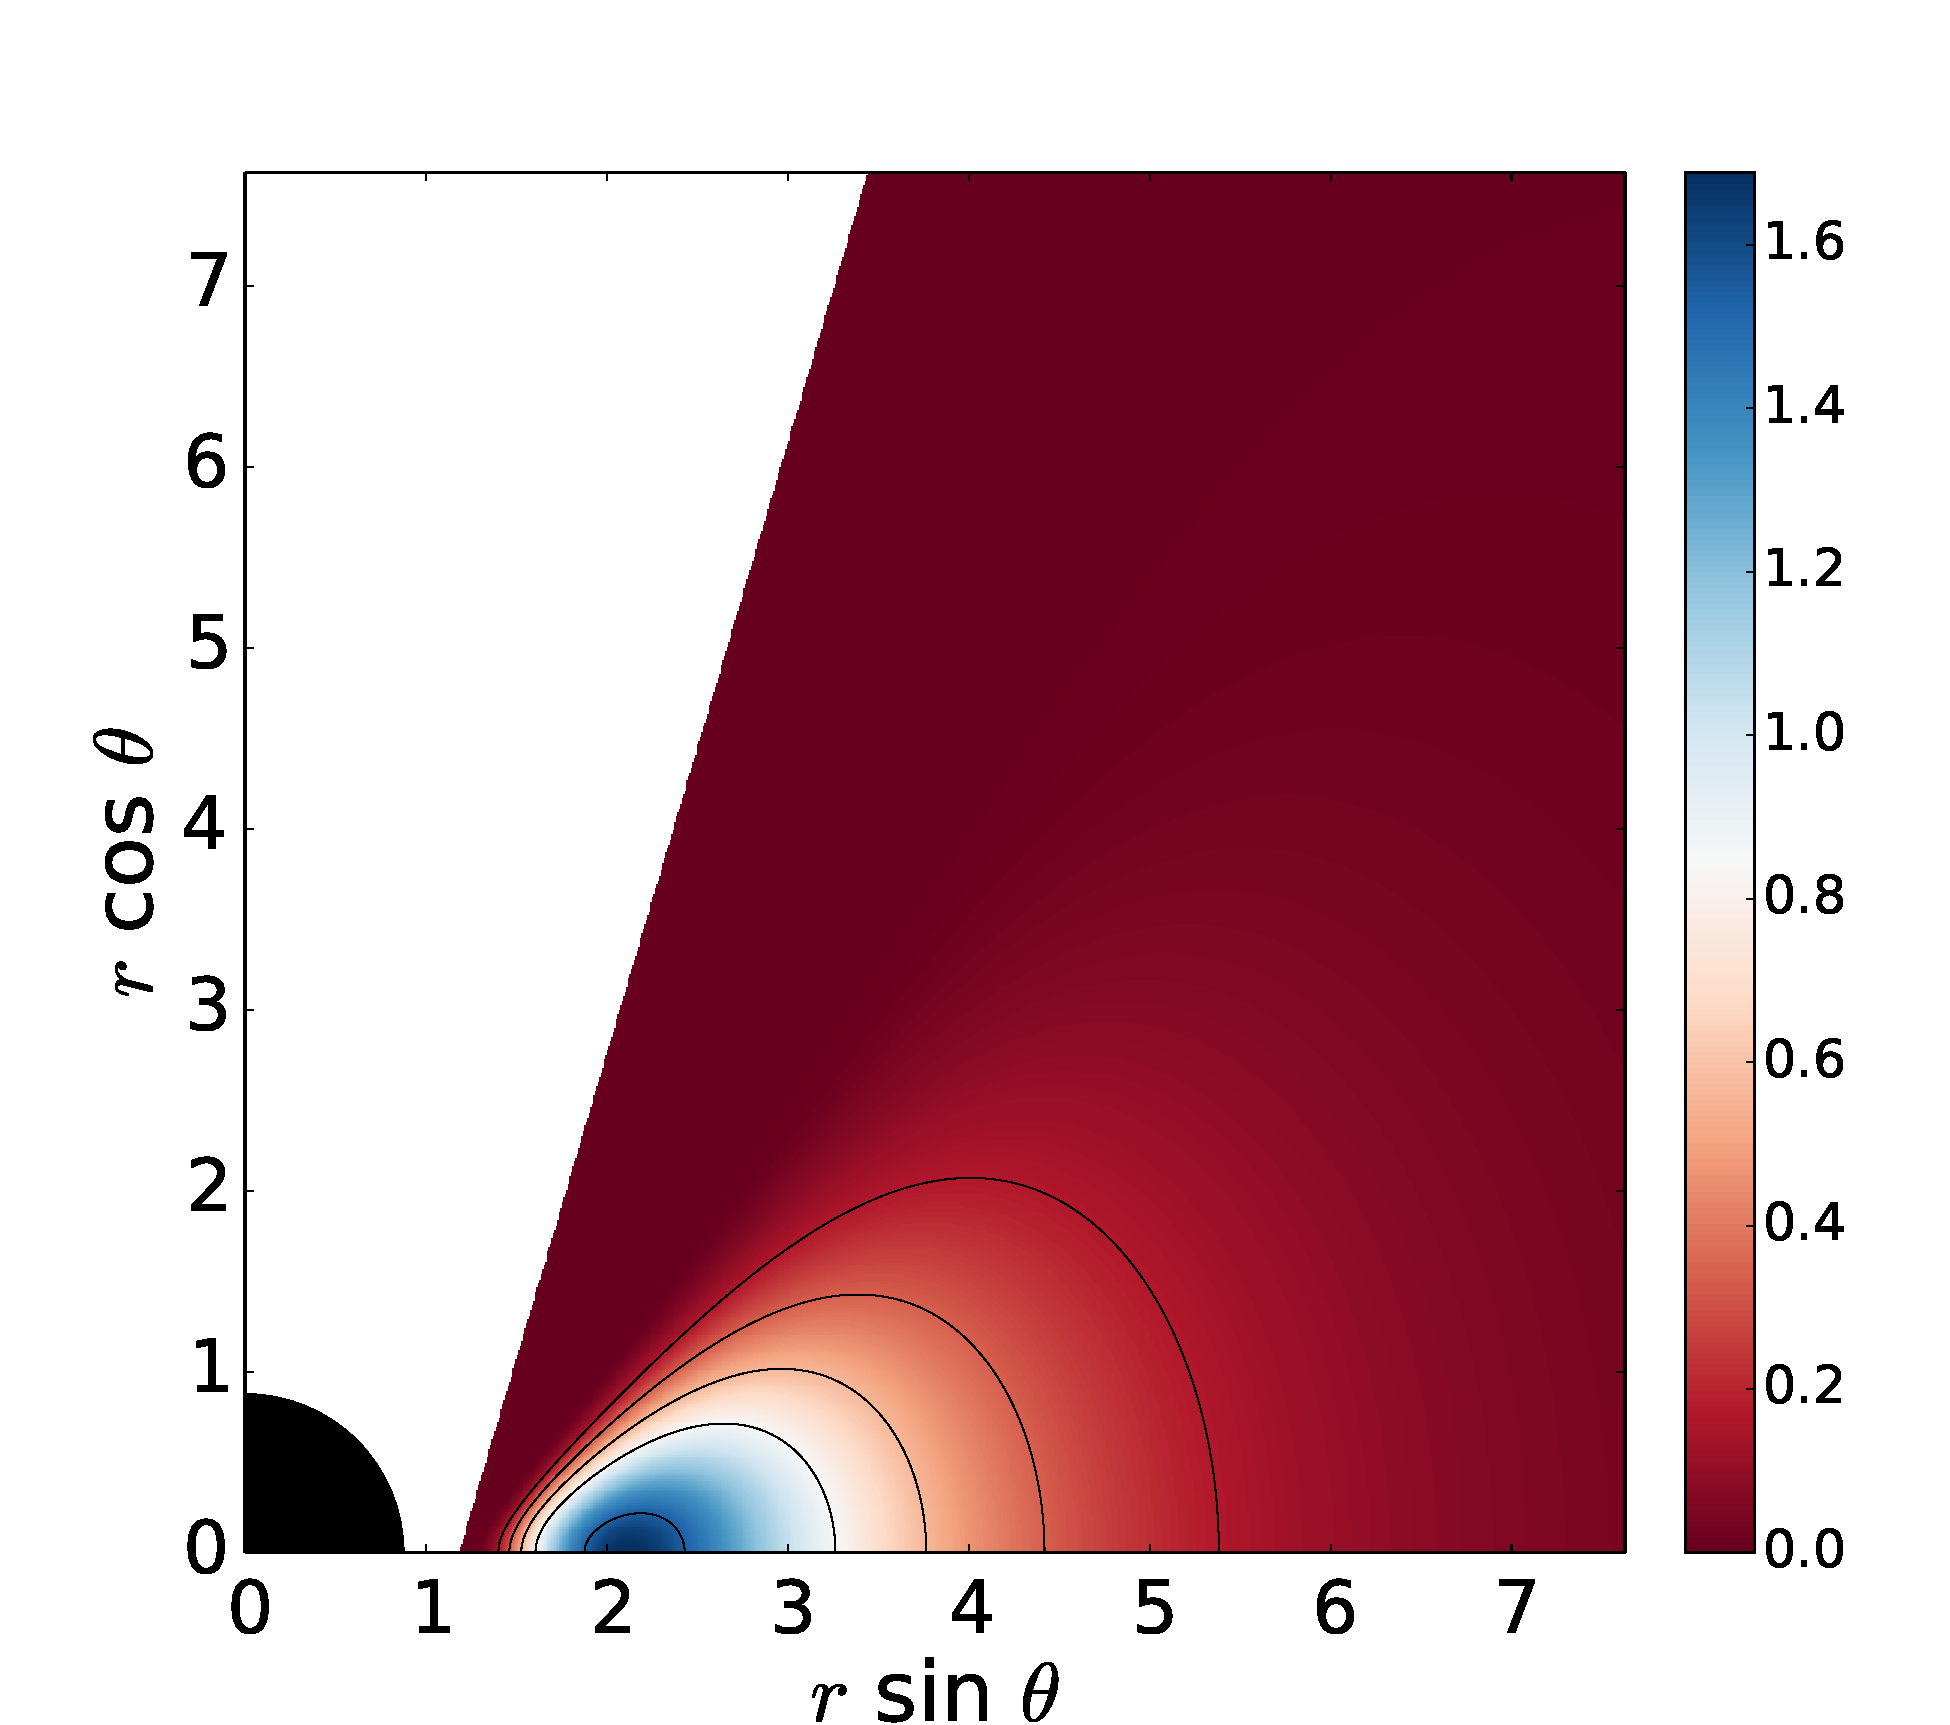
\includegraphics[scale=0.2]{figures/fig4_V_ADM__3.pdf}
\hspace{-0.2cm}
\caption{Rest-mass density distribution for the model III. From top to bottom the rows correspond to the different values of the magnetization parameter, namely non-magnetized ($\beta_{\mathrm{m}_{\mathrm{c}}} = 10^{3}$), mildly magnetized ($\beta_{\mathrm{m}_{\mathrm{c}}} = 1$) and strongly magnetized ($\beta_{\mathrm{m}_{\mathrm{c}}} = 10^{-3}$). The left column correspond to the KBHsSH model and the right column correspond to the corresponding KBH with the same ADM quantities.}
\label{comparison_mag_3}
\end{figure*}

\begin{figure*}
\centering
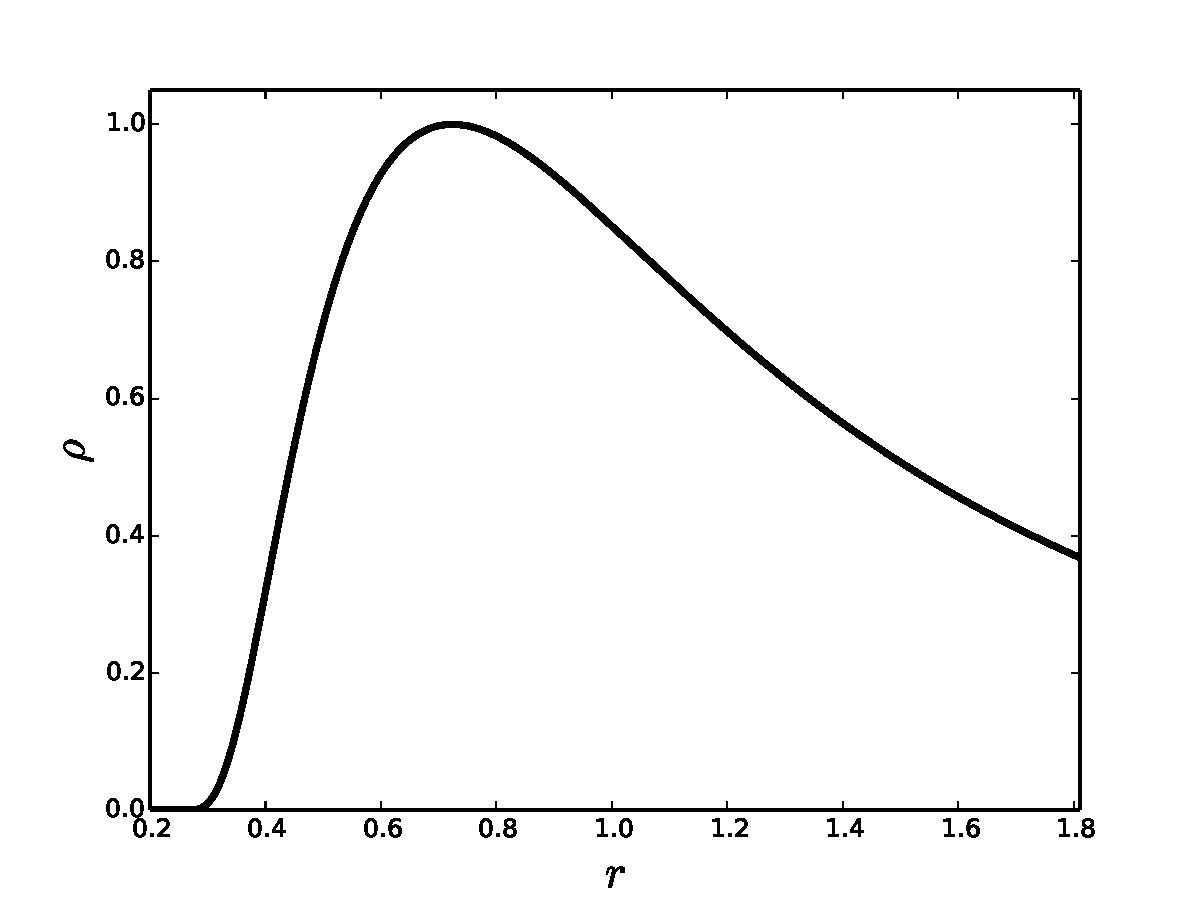
\includegraphics[scale=0.3]{figures/radial_III_HBH_3.pdf}
\hspace{-0.3cm}
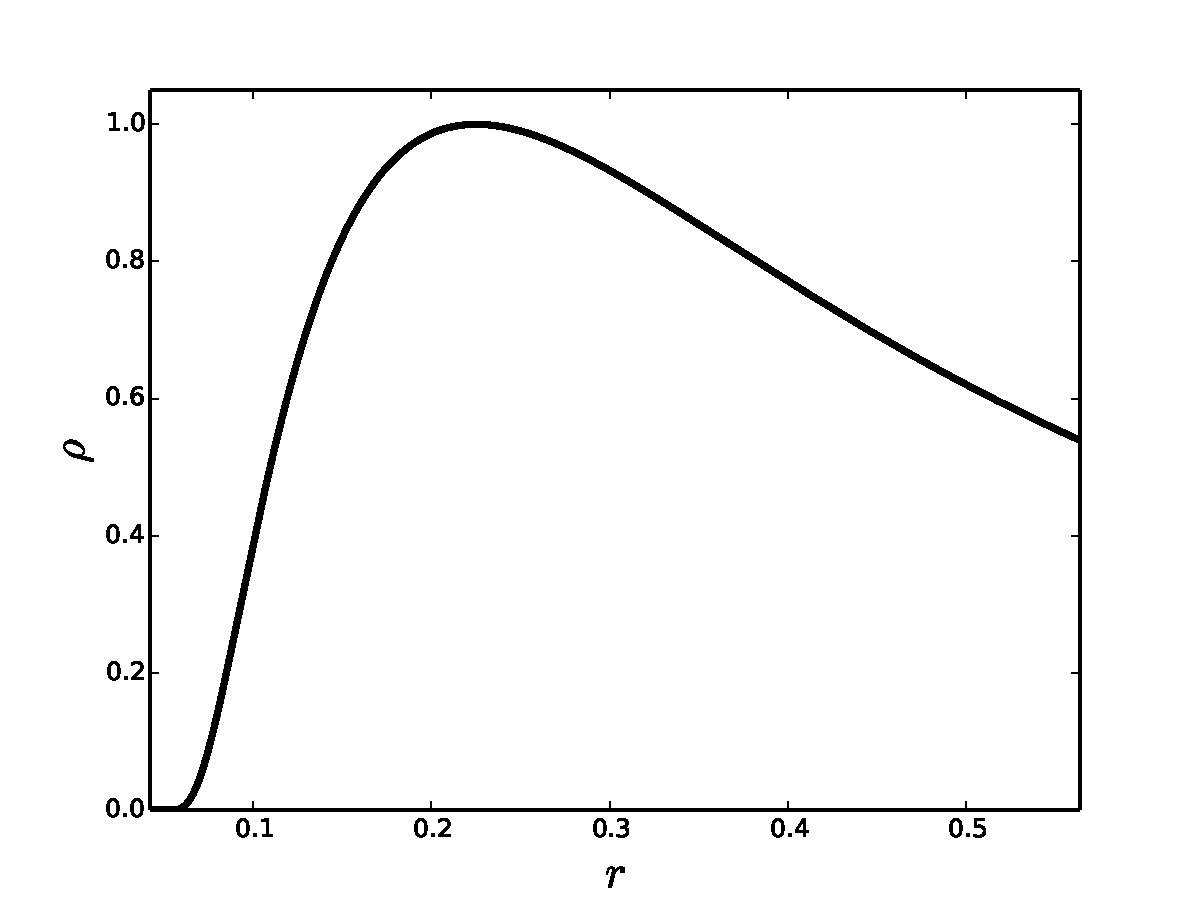
\includegraphics[scale=0.3]{figures/radial_III_ADM_3.pdf}
\hspace{-0.2cm}
\\
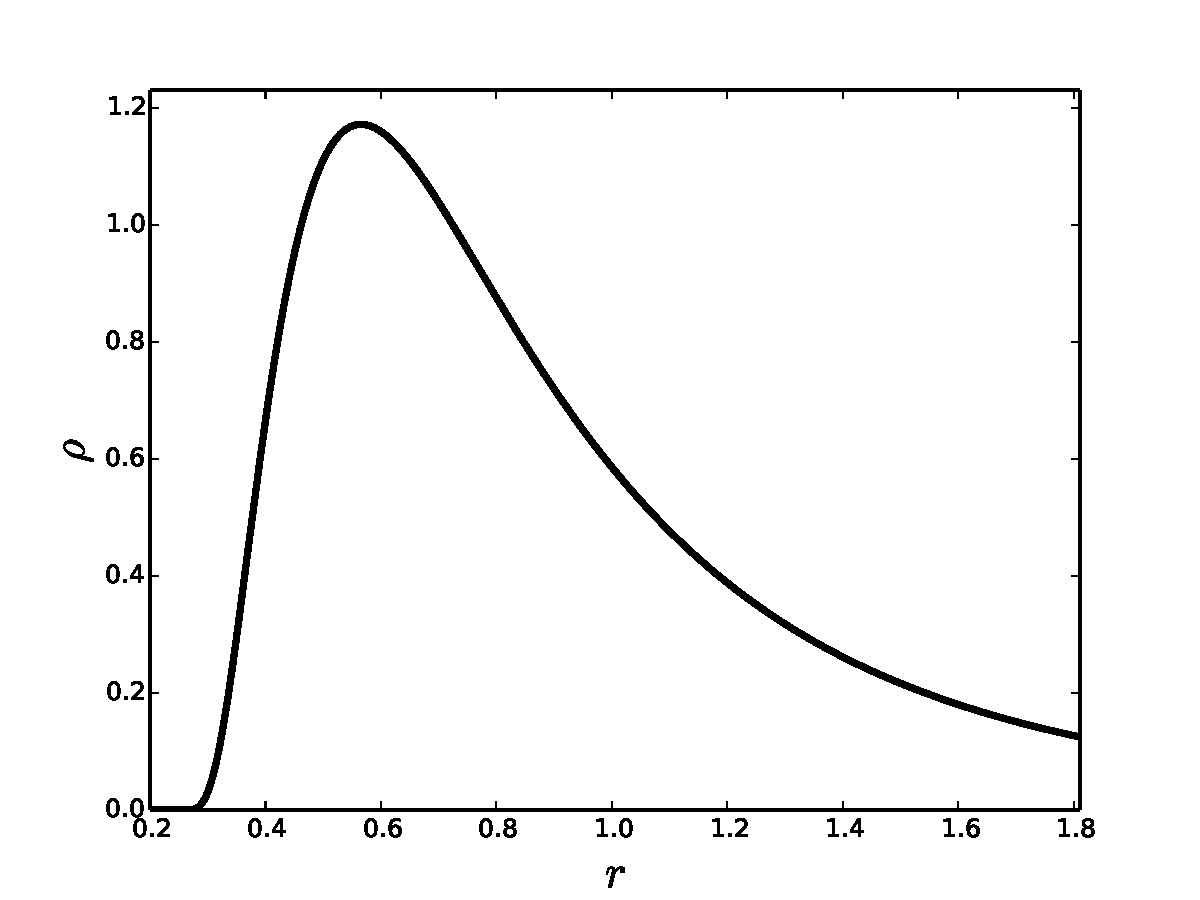
\includegraphics[scale=0.3]{figures/radial_III_HBH_0.pdf}
\hspace{-0.3cm}
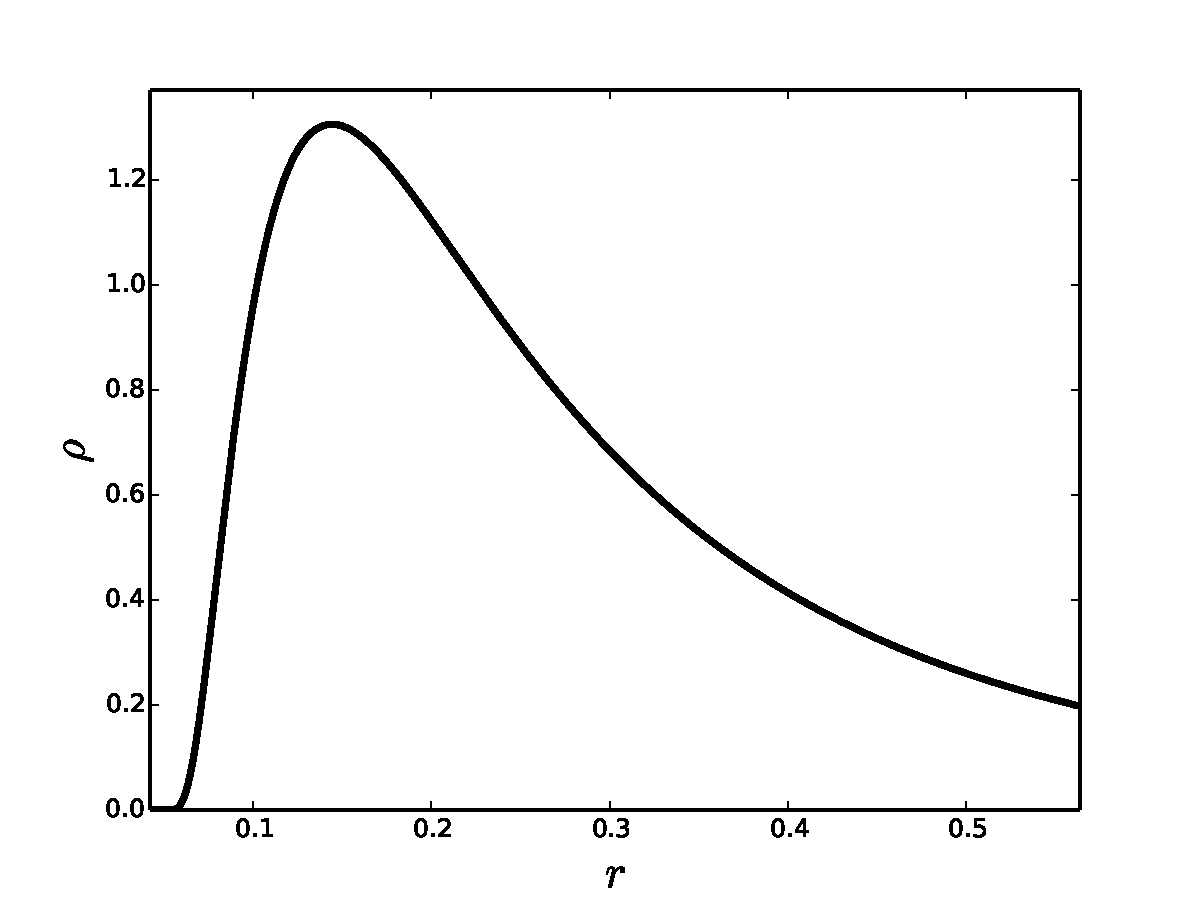
\includegraphics[scale=0.3]{figures/radial_III_ADM_0.pdf}
\hspace{-0.2cm}
\\
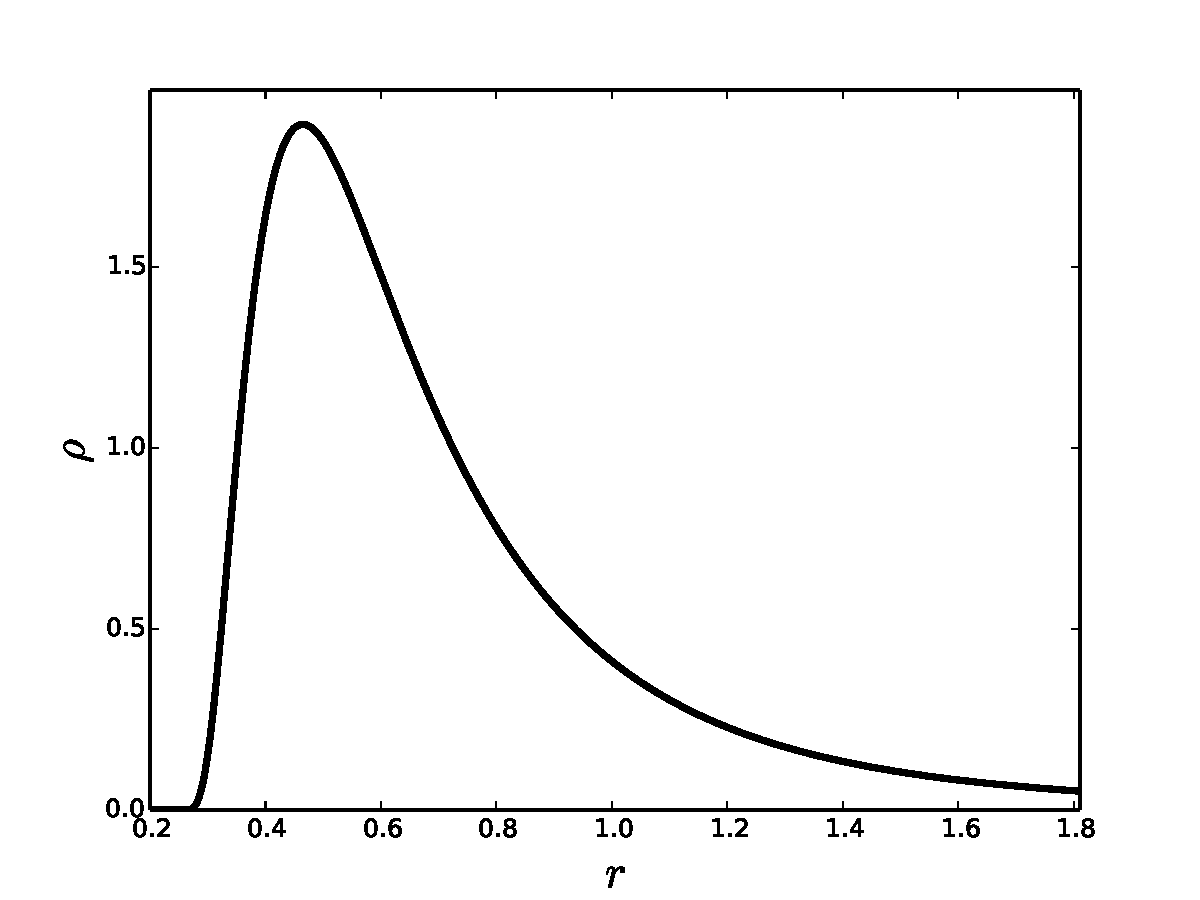
\includegraphics[scale=0.3]{figures/radial_III_HBH__3.pdf}
\hspace{-0.3cm}
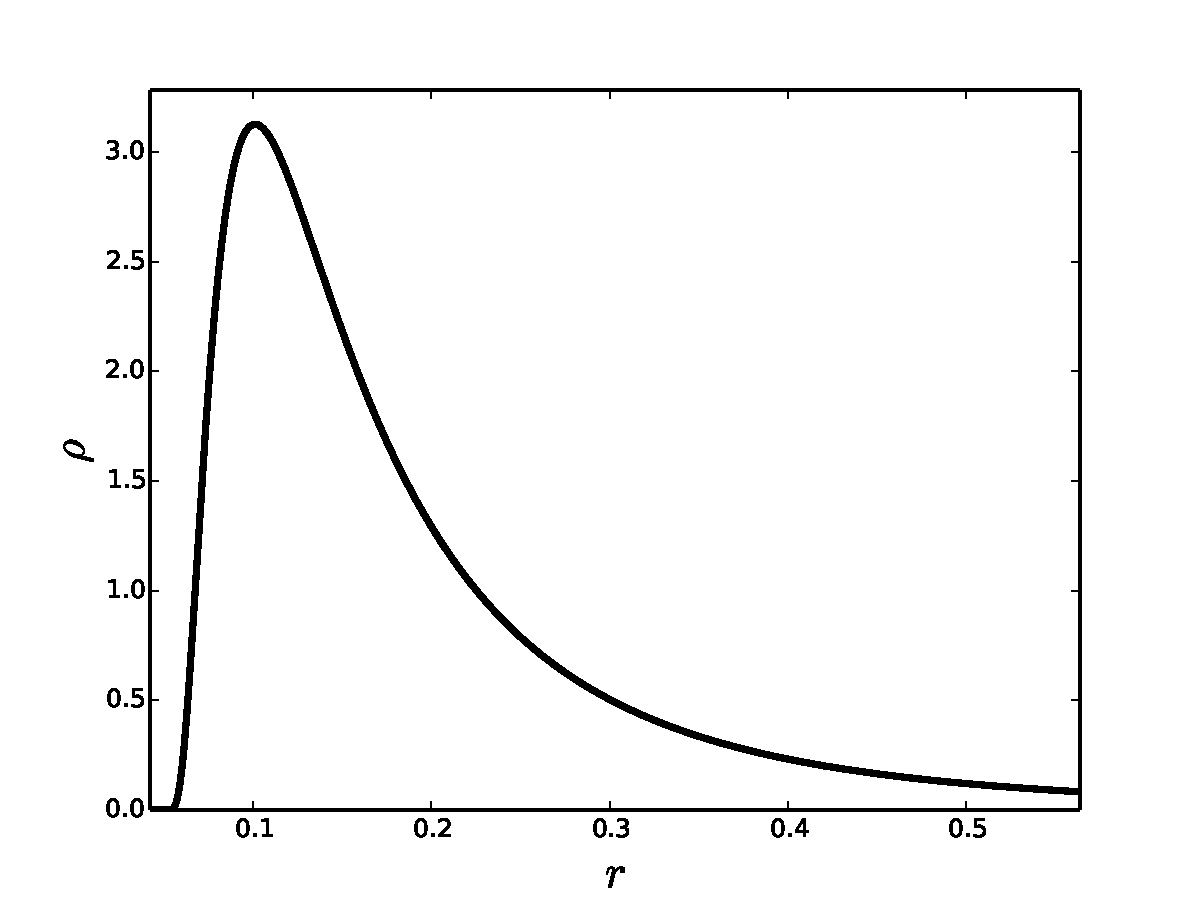
\includegraphics[scale=0.3]{figures/radial_III_ADM__3.pdf}
\hspace{-0.2cm}
\caption{Radial rest-mass density distribution for the model I at the equatorial plane. From top to bottom the rows correspond to the different values of the magnetization parameter, namely non-magnetized ($\beta_{\mathrm{m}_{\mathrm{c}}} = 10^{3}$), mildly magnetized ($\beta_{\mathrm{m}_{\mathrm{c}}} = 1$) and strongly magnetized ($\beta_{\mathrm{m}_{\mathrm{c}}} = 10^{-3}$). The left column correspond to the KBHsSH model and the right column correspond to the corresponding KBH with the same ADM quantities.}
\label{comparison_radial_1}
\end{figure*}

\begin{figure*}
\centering
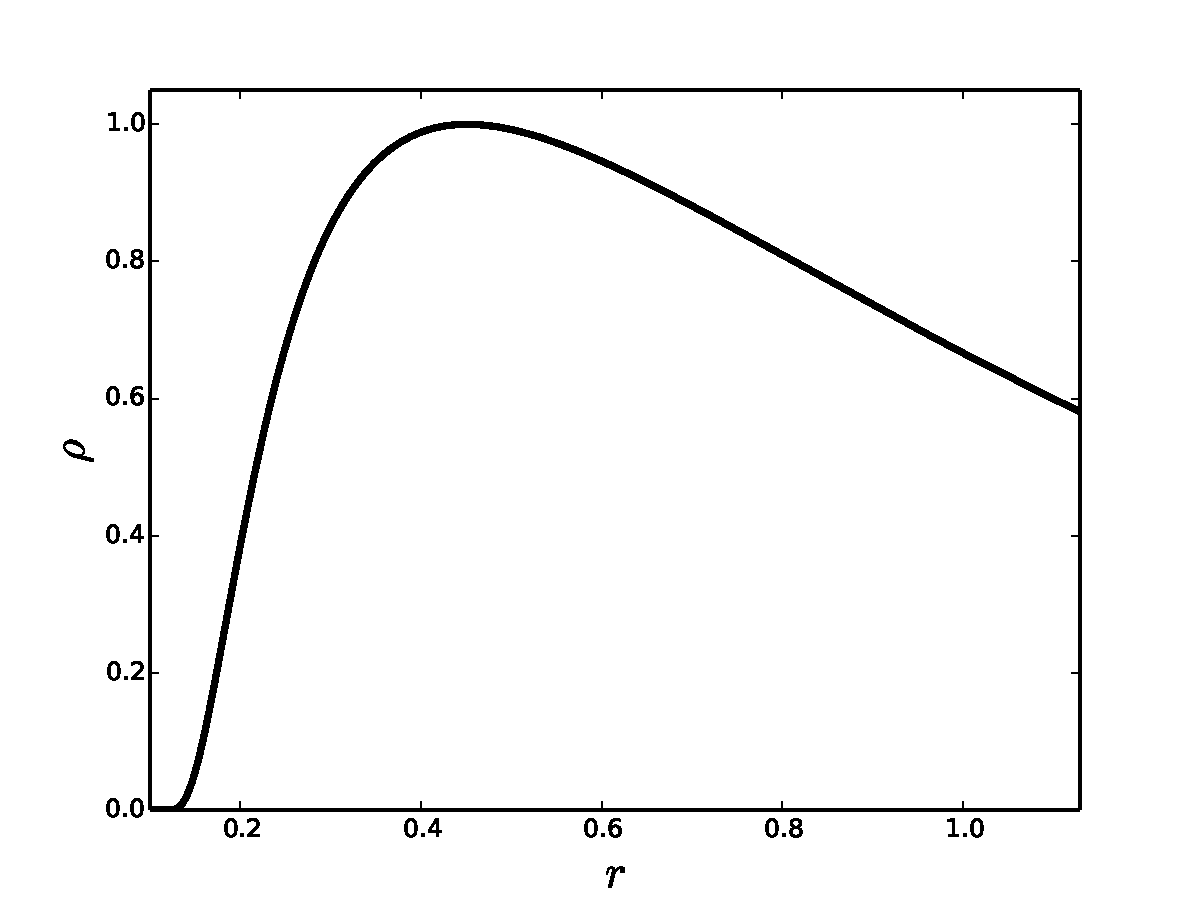
\includegraphics[scale=0.3]{figures/radial_IV_HBH_3.pdf}
\hspace{-0.3cm}
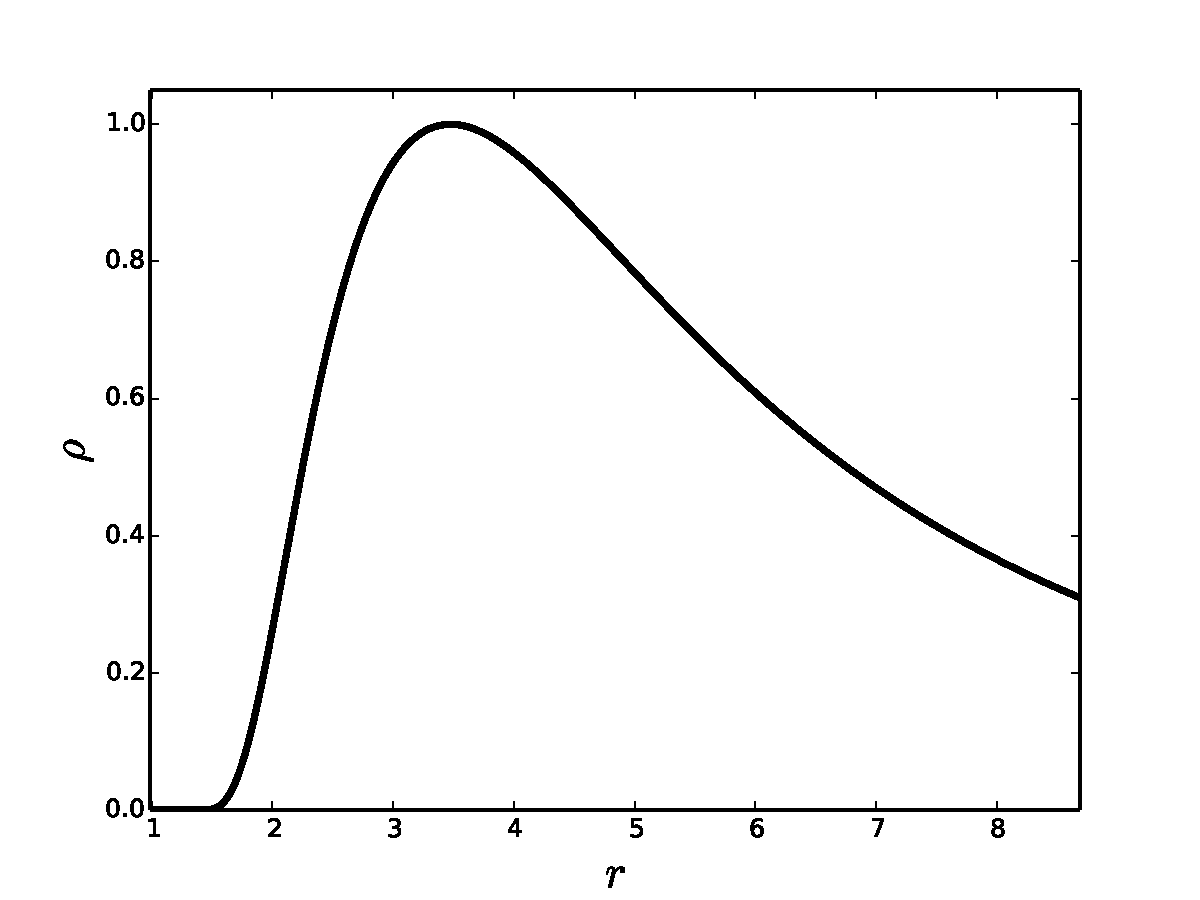
\includegraphics[scale=0.3]{figures/radial_IV_ADM_3.pdf}
\hspace{-0.2cm}
\\
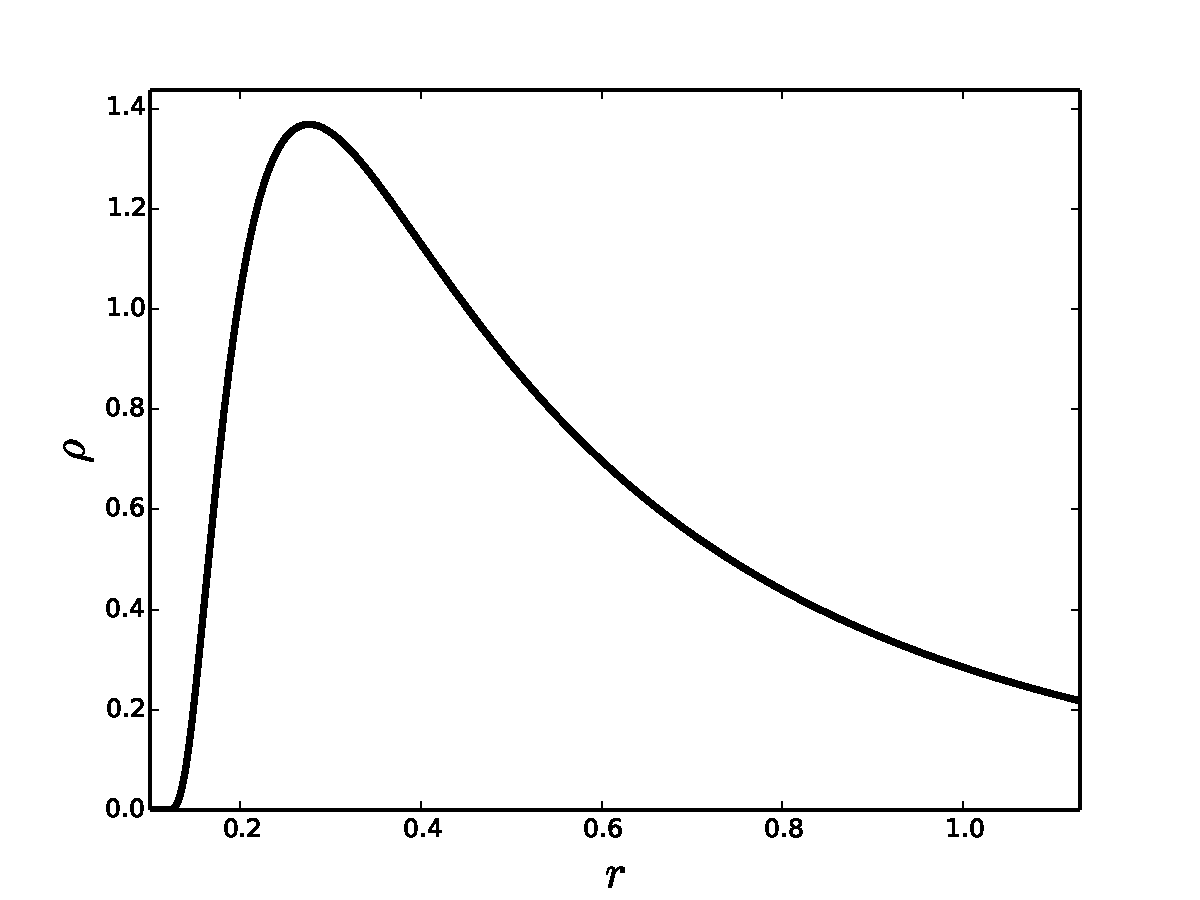
\includegraphics[scale=0.3]{figures/radial_IV_HBH_0.pdf}
\hspace{-0.3cm}
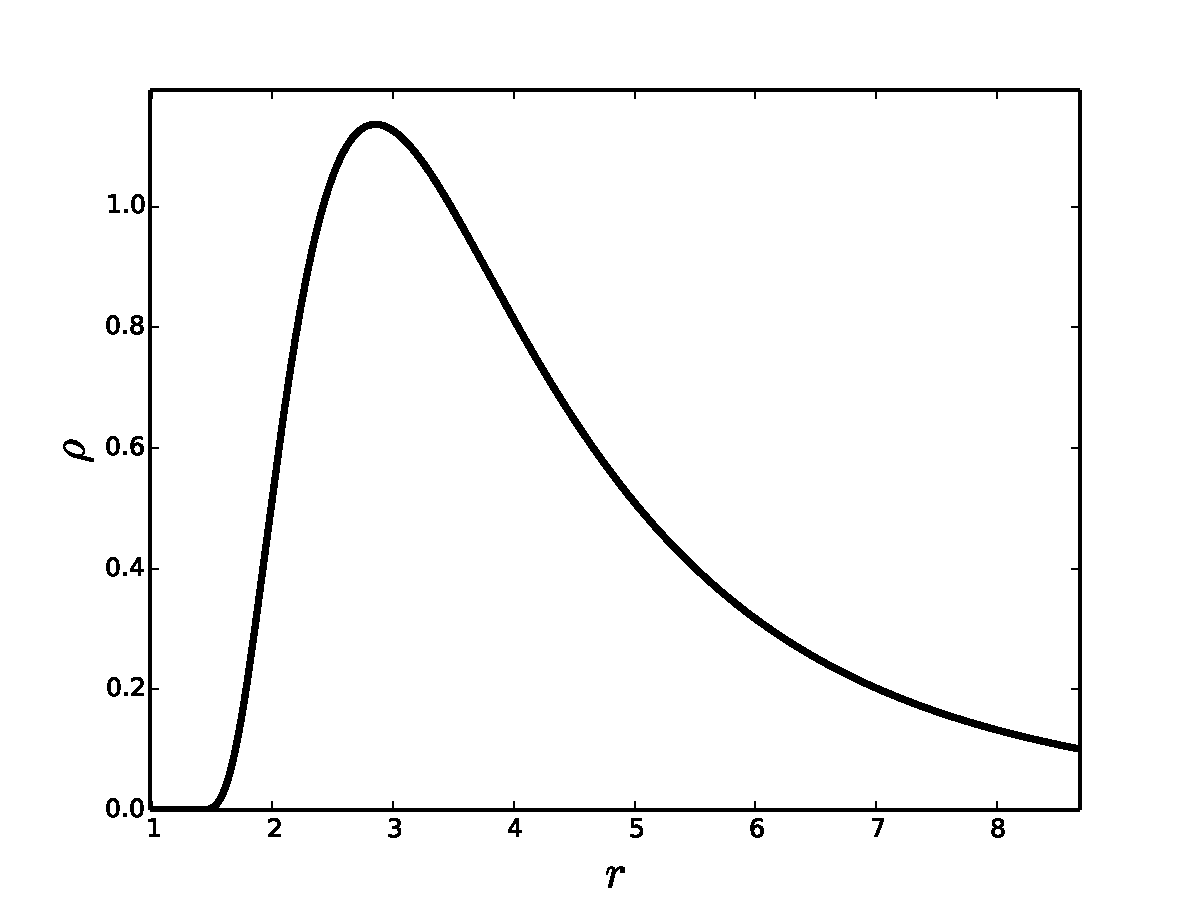
\includegraphics[scale=0.3]{figures/radial_IV_ADM_0.pdf}
\hspace{-0.2cm}
\\
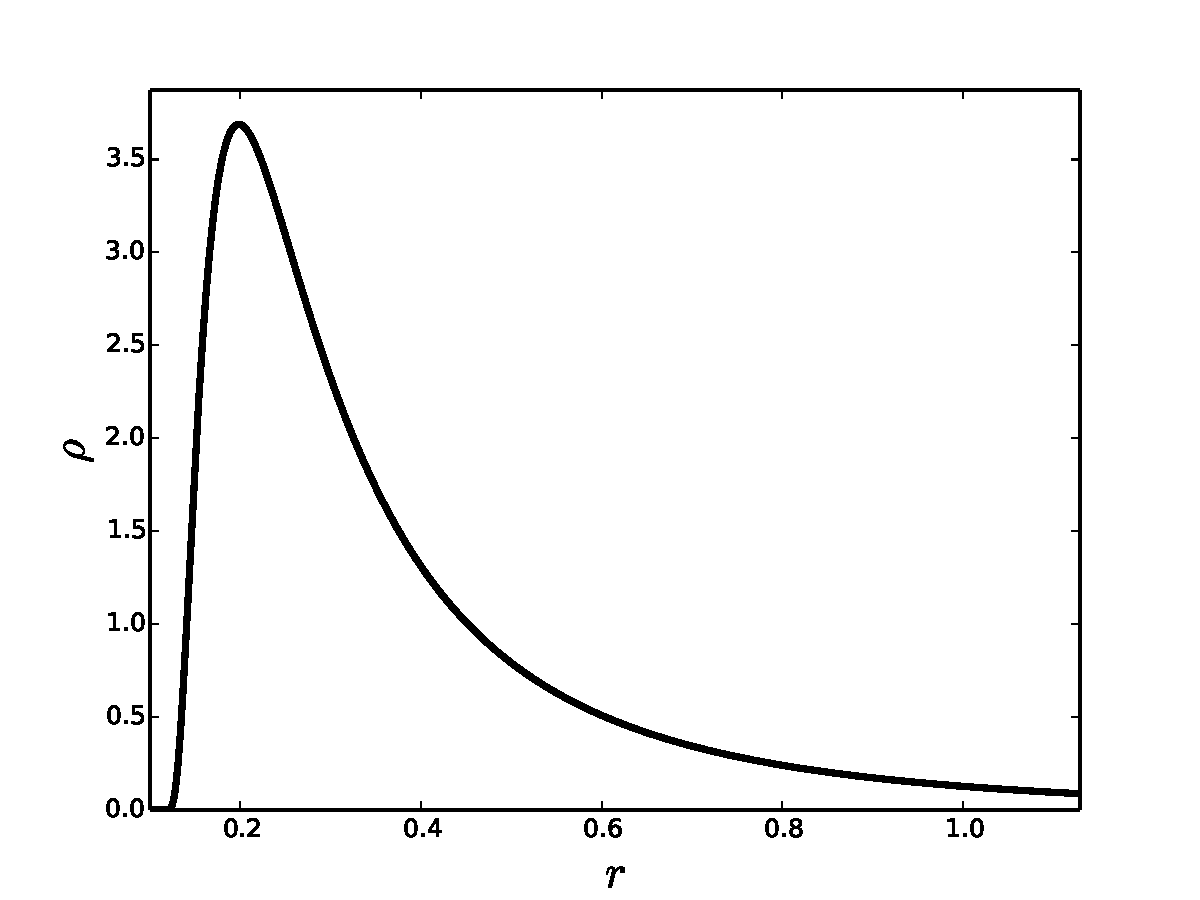
\includegraphics[scale=0.3]{figures/radial_IV_HBH__3.pdf}
\hspace{-0.3cm}
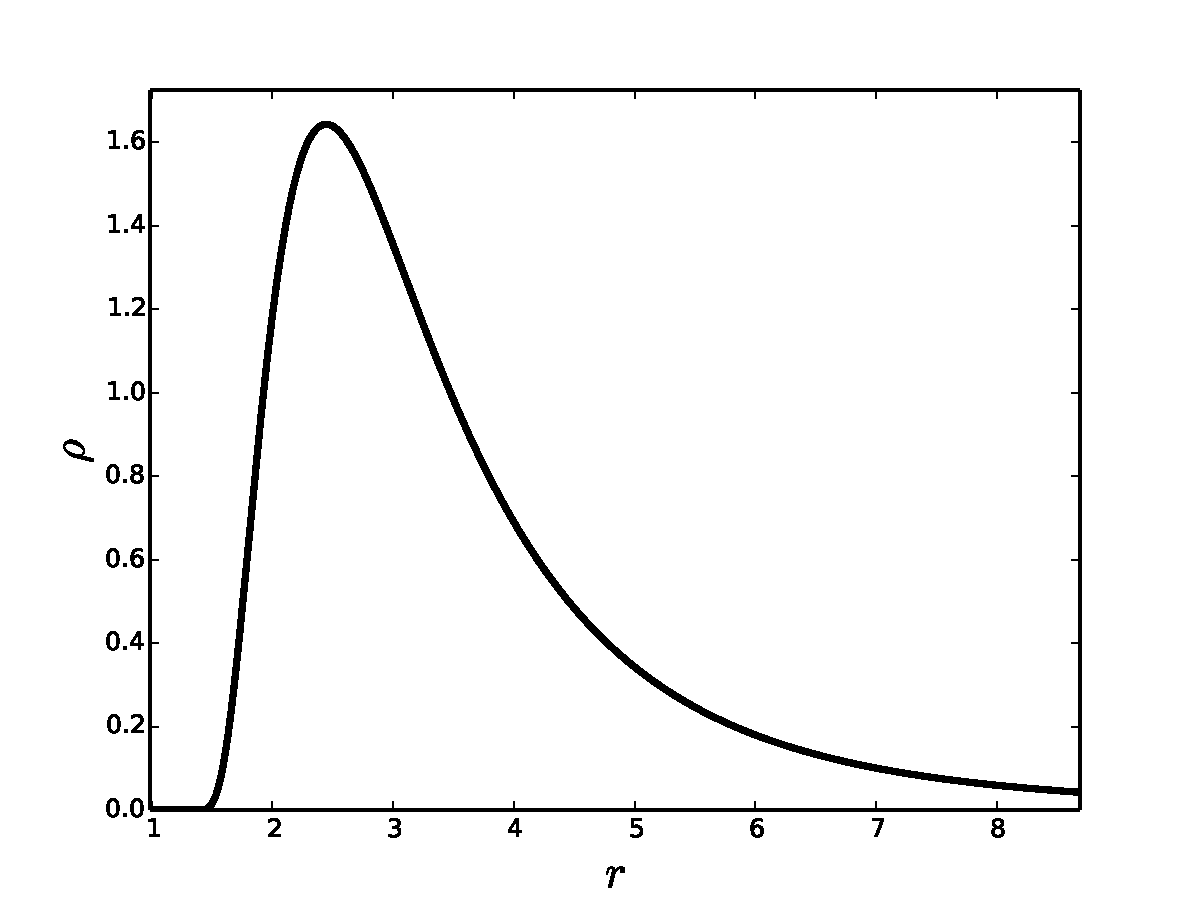
\includegraphics[scale=0.3]{figures/radial_IV_ADM__3.pdf}
\hspace{-0.2cm}
\caption{Radial rest-mass density distribution for the model II at the equatorial plane. From top to bottom the rows correspond to the different values of the magnetization parameter, namely non-magnetized ($\beta_{\mathrm{m}_{\mathrm{c}}} = 10^{3}$), mildly magnetized ($\beta_{\mathrm{m}_{\mathrm{c}}} = 1$) and strongly magnetized ($\beta_{\mathrm{m}_{\mathrm{c}}} = 10^{-3}$). The left column correspond to the KBHsSH model and the right column correspond to the corresponding KBH with the same ADM quantities.}
\label{comparison_radial_2}
\end{figure*}

\begin{figure*}
\centering
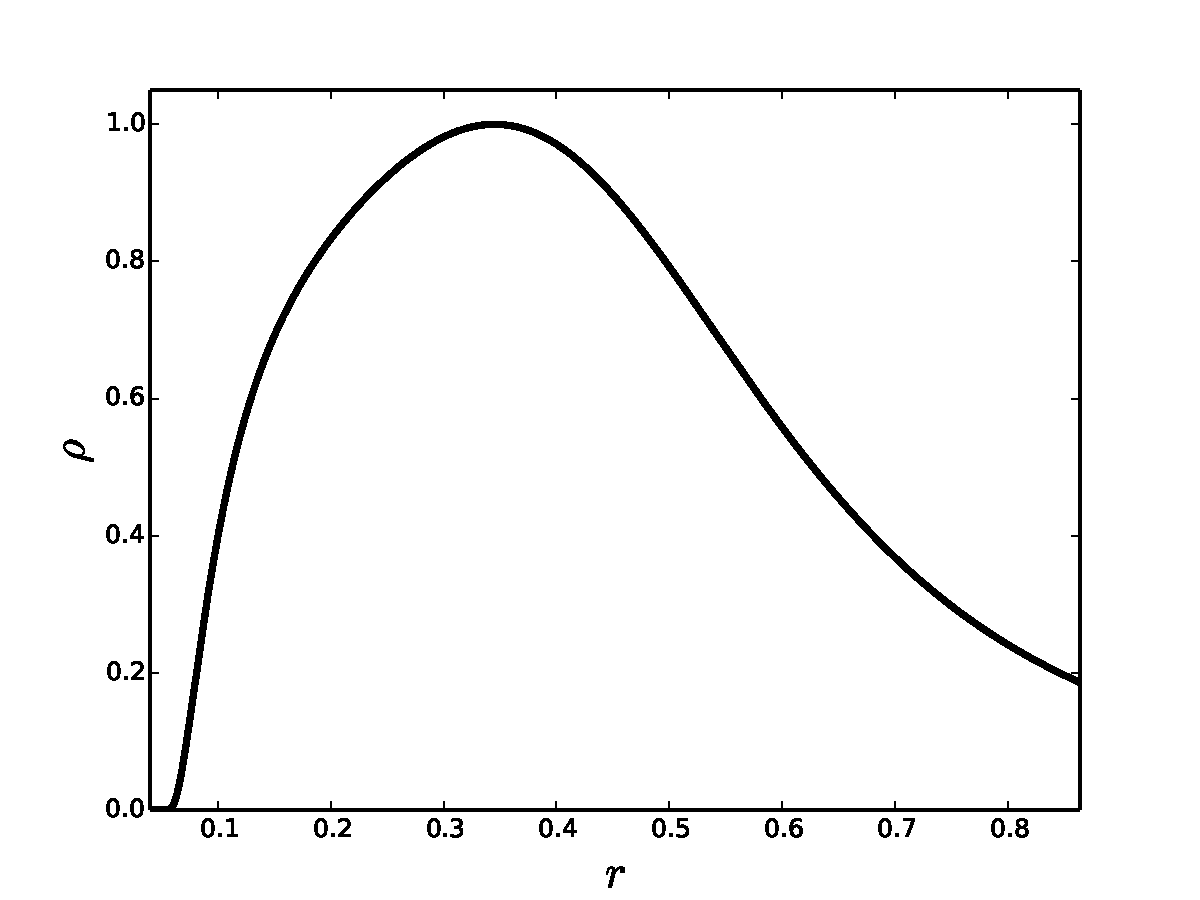
\includegraphics[scale=0.3]{figures/radial_V_HBH_3.pdf}
\hspace{-0.3cm}
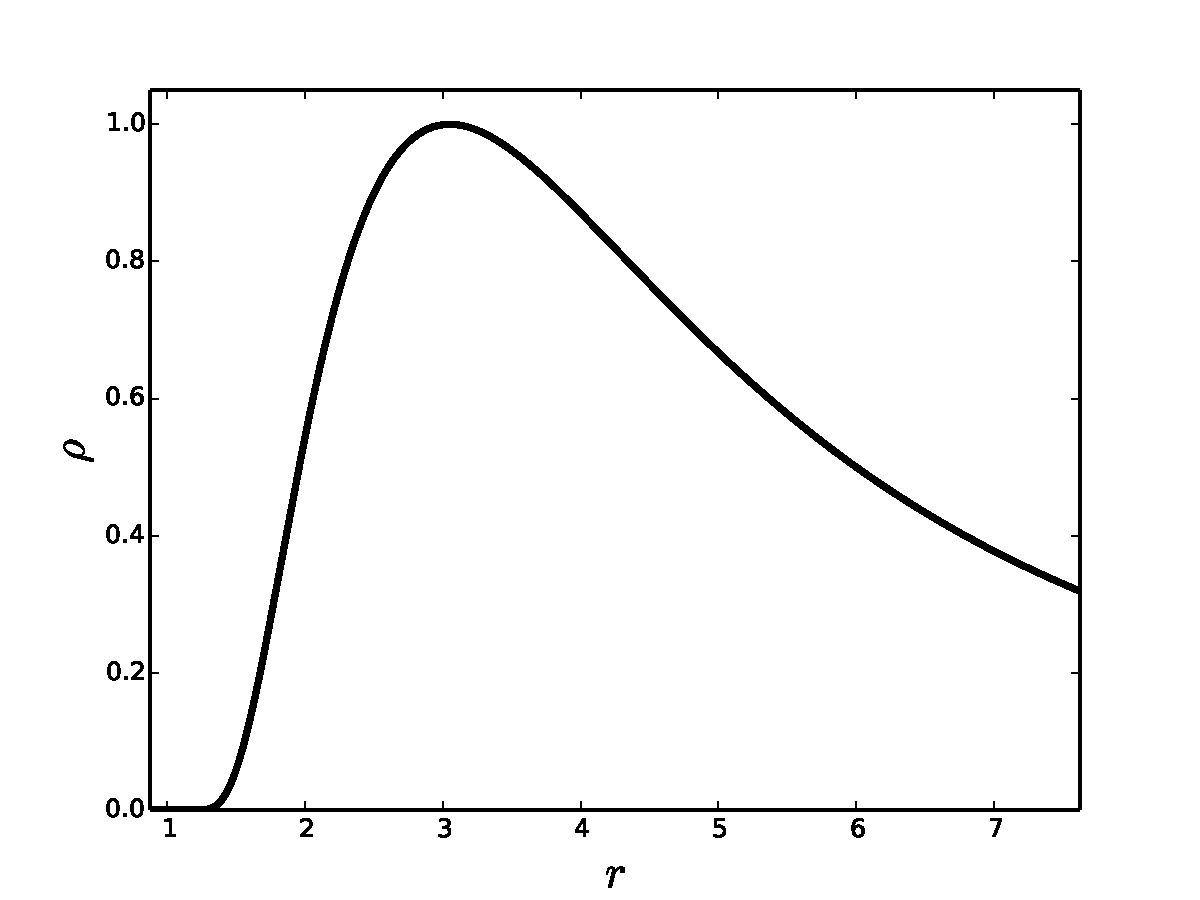
\includegraphics[scale=0.3]{figures/radial_V_ADM_3.pdf}
\hspace{-0.2cm}
\\
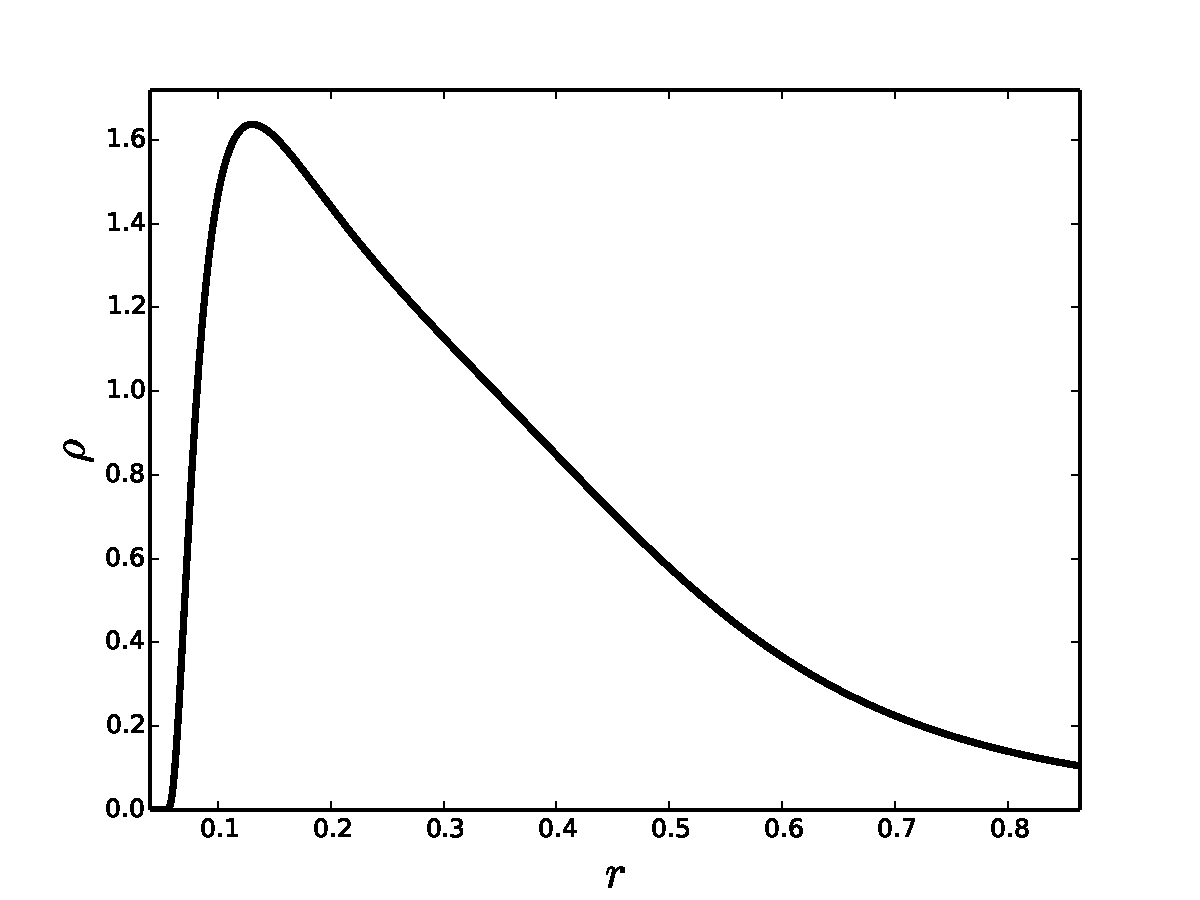
\includegraphics[scale=0.3]{figures/radial_V_HBH_0.pdf}
\hspace{-0.3cm}
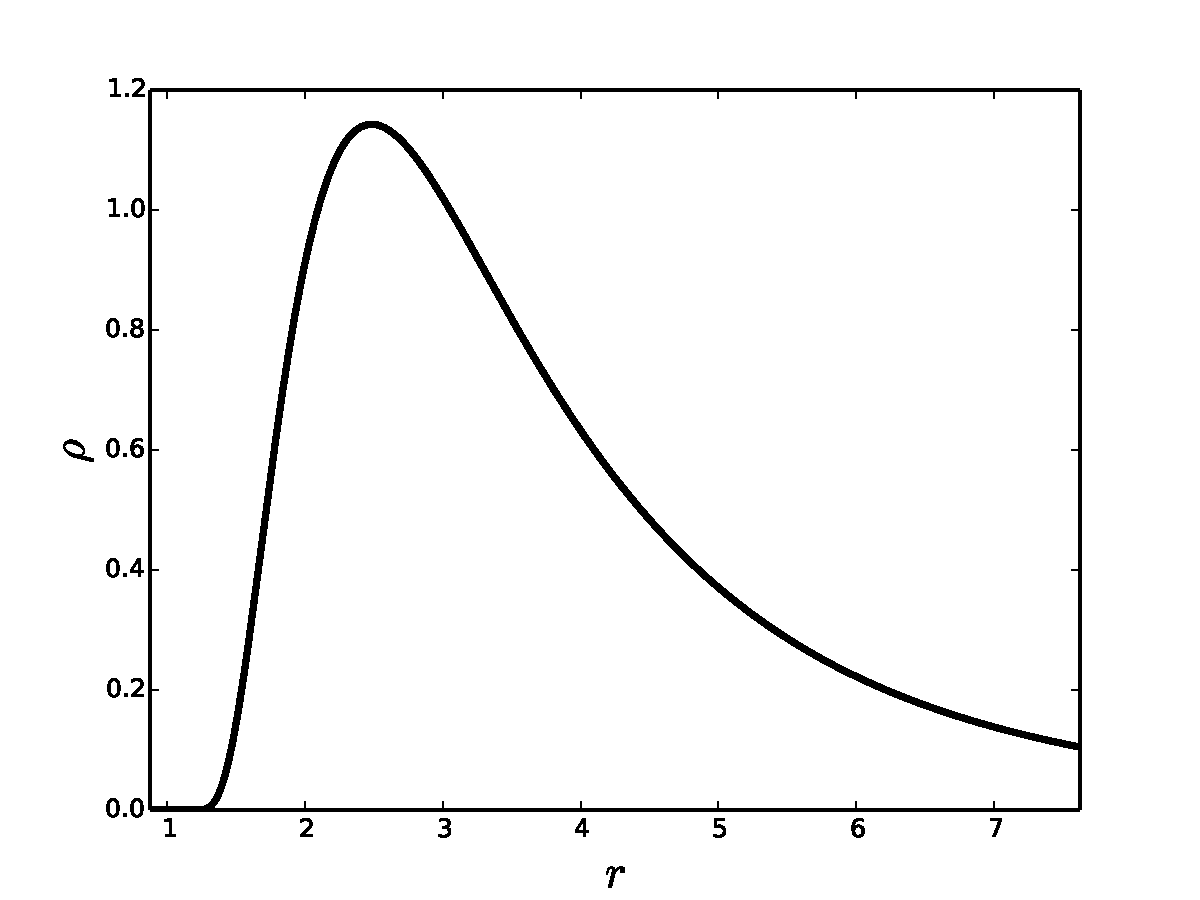
\includegraphics[scale=0.3]{figures/radial_V_ADM_0.pdf}
\hspace{-0.2cm}
\\
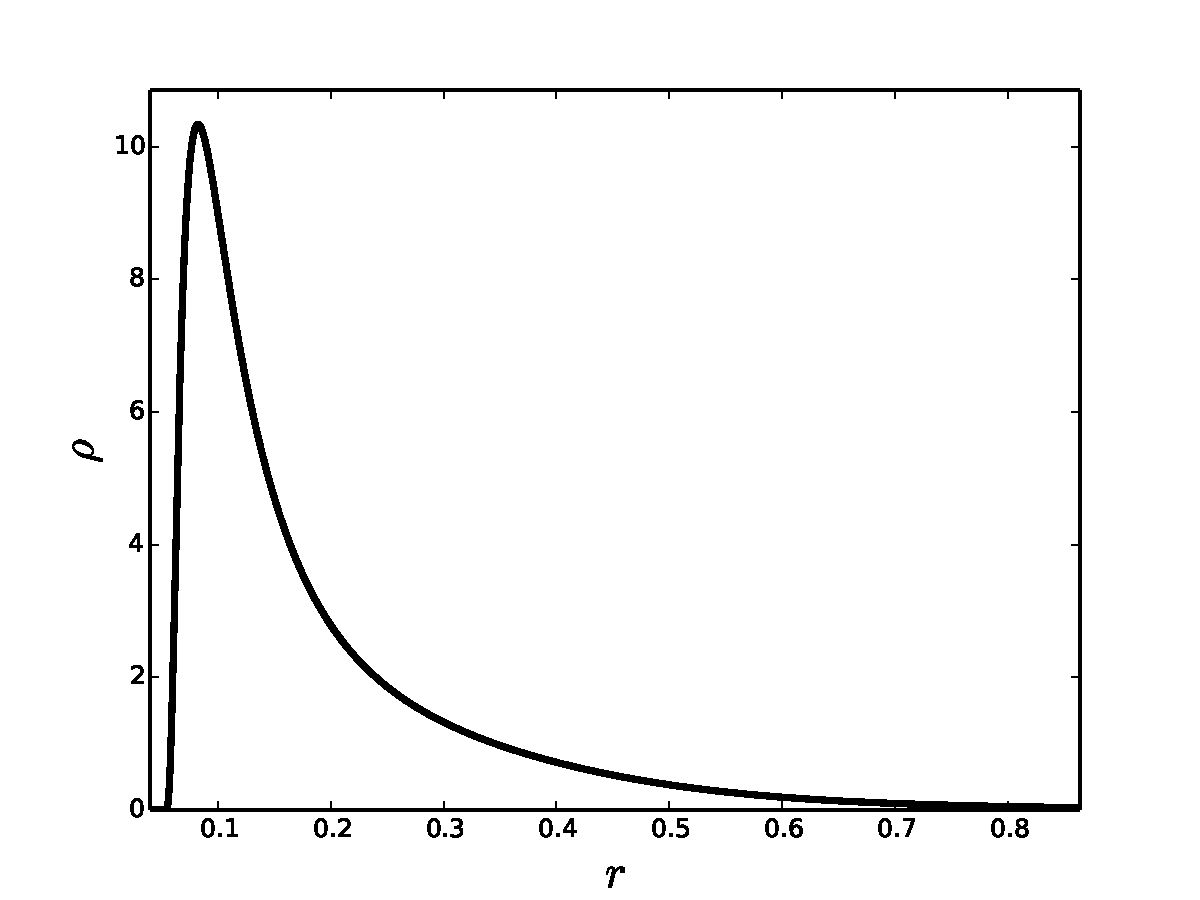
\includegraphics[scale=0.3]{figures/radial_V_HBH__3.pdf}
\hspace{-0.3cm}
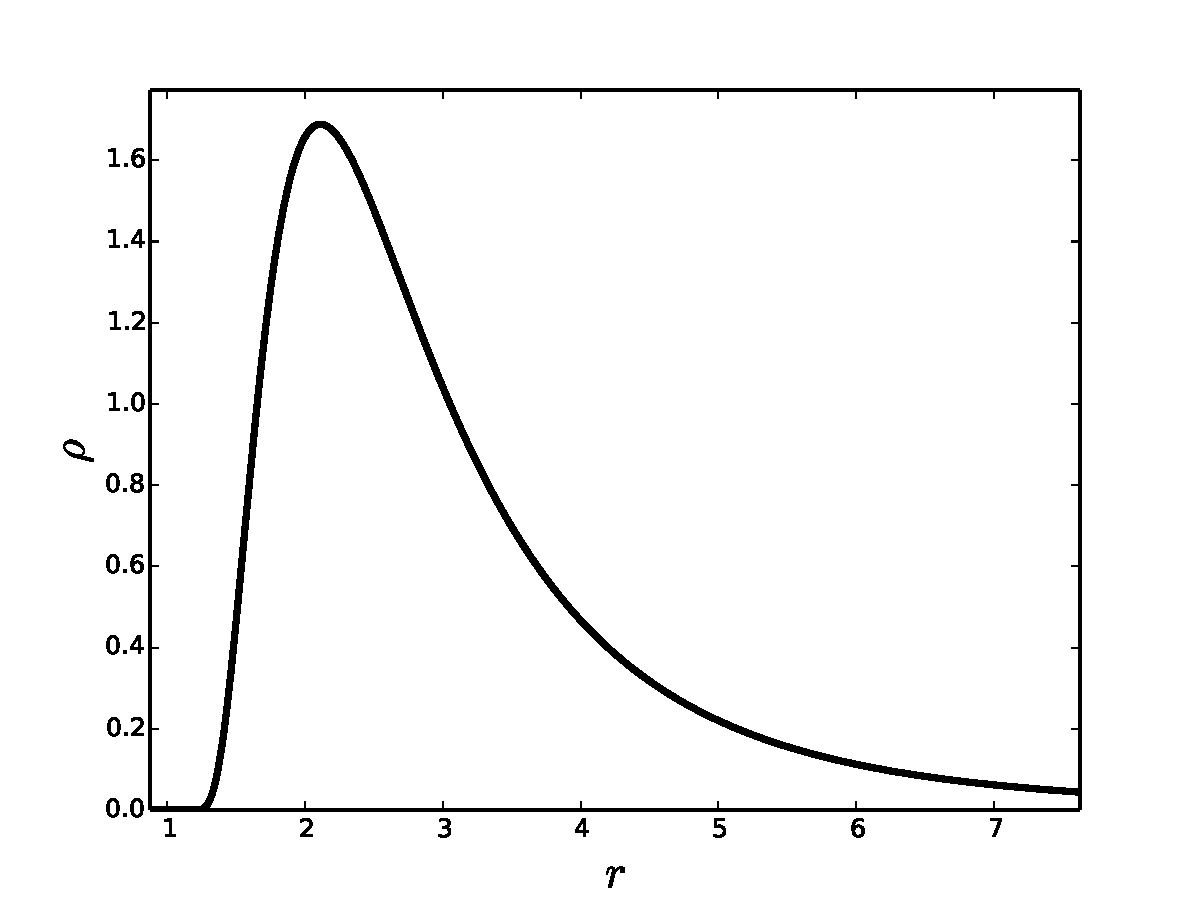
\includegraphics[scale=0.3]{figures/radial_V_ADM__3.pdf}
\hspace{-0.2cm}
\caption{Radial rest-mass density distribution for the model III at the equatorial plane. From top to bottom the rows correspond to the different values of the magnetization parameter, namely non-magnetized ($\beta_{\mathrm{m}_{\mathrm{c}}} = 10^{3}$), mildly magnetized ($\beta_{\mathrm{m}_{\mathrm{c}}} = 1$) and strongly magnetized ($\beta_{\mathrm{m}_{\mathrm{c}}} = 10^{-3}$). The left column correspond to the KBHsSH model and the right column correspond to the corresponding KBH with the same ADM quantities.}
\label{comparison_radial_3}
\end{figure*}

\subsection{Distribution of angular momentum and equations of motion}
We consider a constant angular momentum distribution $l(r,\theta) = \mathrm{cte}.$. The specific value of the angular momentum is computed as the minimum of the following equation
\begin{equation}
l^{\pm}_{\mathrm{b}}(r, \theta) = \frac{g_{t\phi}\pm\left(\sqrt{g_{t\phi}^2-g_{tt}g_{t\phi}}\right)\sqrt{1+g_{tt}}}{-g_{tt}}
\end{equation}
where the plus sign is for prograde orbits and the minus is for retrograde orbits.
This expression is given by~\citep{Daigne:2004} for Kerr BHs, but it is valid for any stationary, axisymmetric spacetimes. For prograde motion, the function has a minimum outside the event horizon. The location of said minimum corresponds with the marginally bound orbit $r_{\mathrm{mb}}$, and the angular momentum corresponds to the keplerian angular momentum at that point. This choice of angular momentum distributions is motivated by its simplicity (for a first study of thick tori around KBHsSH) and for allowing the presence of a cusp (this allows matter accretion onto the black hole) and a centre.


\subsection{Magnetized disks}
We use the procedure described by~\citet{Montero:2007}, where we write the equations of ideal general relativistic MHD are the following conservation laws, $\nabla_{\mu} T^{\mu\nu} = 0$, $\nabla_{\mu} \,^\ast F^{\mu\nu} = 0$, and 
$\nabla_{\mu} (\rho u^{\mu}) = 0$, 
where $\nabla_{\mu}$ is the covariant derivative and
\begin{equation}\label{eq:e-m_tensor}
T^{\mu\nu} = (\rho h + b^2)u^{\mu}u^{\nu} + \left(p + \frac{1}{2}b^2\right)g^{\mu\nu} - b^{\mu}b^{\nu},
\end{equation}
is the energy-momentum tensor of a magnetised perfect fluid, $h$, $\rho$ $p$ being the fluid specific enthalpy, density and fluid pressure, respectively. 
Moreover, $^\ast F^{\mu\nu} = b^{\mu}u^{\nu} - b^{\nu}u^{\mu}$ is the (dual of the) Faraday tensor relative to an observer with 
four-velocity $u^{\mu}$, and $b^{\mu}$ is the magnetic field in that frame, with
$b^2=b^{\mu}b_{\mu}$. Assuming the magnetic field is purely azimuthal, i.e.~$b^r = b^{\theta} = 0$,
and taking into account that the flow is stationary and axisymmetric, the conservation of the current density and of the Faraday tensor follow. Contracting the divergence of Eq.~\eqref{eq:e-m_tensor} with the projection tensor $h^{\alpha}_{\,\,\beta} = \delta^{\alpha}_{\,\,\beta} + u^{\alpha}u_{\beta}$, we arrive at
\begin{equation}
(\rho h + b^2)u_{\nu}\partial_i u^{\nu} + \partial_i\left(p + \frac{b^2}{2}\right) - b_{\nu}\partial_i b^{\nu}=0\,,
\end{equation}
where $i = r, \theta$. Then, we rewrite this equation in terms of the specific angular momentum $l$ and of the angular velocity $\Omega$, to obtain
\begin{equation}\label{eq:diff_ver}
\partial_i(\ln u_t|) - \frac{\Omega \partial_i l}{1-l\Omega} + \frac{\partial_i p}{w} + \frac{\partial_i(\mathcal{L}b^2)}{2\mathcal{L}w} = 0\,,
\end{equation}
where $\mathcal{L} = g_{t\phi}^2 - g_{tt}g_{\phi\phi}$.
To integrate Eq.~\eqref{eq:diff_ver} we first assume a polytropic equation of state of the form
\begin{equation}\label{eq:eos_fluid}
p = K \rho^{\Gamma},
\end{equation}
with $K$ and $\Gamma$ constants.
Then, we define the magnetic pressure as $p_{\mathrm{m}} = b^2/2$, and introduce the definitions $\tilde{p}_{\mathrm{m}} = \mathcal{L} p_{\mathrm{m}}$ and $\tilde{w} = \mathcal{L} w$, in order to write an analogue equation to Eq.~\eqref{eq:eos_fluid} for $\tilde{p}_{\mathrm{m}}$~\citep{Komissarov:2006}
\begin{equation}\label{eq:eos_mag_tilde}
\tilde{p}_{\mathrm{m}} = M \tilde{w}^q,
\end{equation}
or, in terms of the magnetic pressure $p_{\mathrm{m}}$
\begin{equation}\label{eq:eos_mag}
p_{\mathrm{m}} = M \mathcal{L}^{q-1} w^q,
\end{equation}
where $w = \rho h$ is the fluid enthaply density, and $M$ and $q$ are constants.
If we define the potential as $W \equiv \ln u_t|$, then we can integrate the equation~\eqref{eq:diff_ver} as

\begin{equation}\label{eq:final}
W - W_{\mathrm{in}} + \ln \left(1 + \frac{\Gamma K}{\Gamma +1}\rho^{\gamma -1}\right) + \frac{q}{q-1}M(\mathcal{L}w)^{q-1}=0,
\end{equation}
where $W_{\mathrm{in}}$ is the potential at the inner edfe of the disk.

In this work, we use $q = \Gamma = 4/3$, the density at the disk centre $\rho_{\mathrm{c}} = 1$ and the angular momentum distribution gives us $W_{\mathrm{in}} = 0$. With this information we can compute all the relevant physical quantities.

It is relevant to note that we could have used the framework described by~\citet{Komissarov:2006}. As we will show in appendix~\ref{komissarov_appendix}, we do not take this approach because it is not appropriate for some cases of KBHsSH.

%--------------------------------------------------------------------
\section{Method}

\subsection{Building the disk}

\subsection{Numerical method}

%--------------------------------------------------------------------
\section{Results}

\begin{table}
\caption{List of models of KBHsSH.}             
\label{table:1}      
\centering          
\begin{tabular}{c c c c  c c c c}
\hline\hline       
 & $M_{\mathrm{ADM}}$ & $J_{\mathrm{ADM}}$ & $M_{\mathrm{H}}$ &  $J_{\mathrm{H}}$ & $M_{\mathrm{SF}}$ & $J_{\mathrm{SF}}$ & $r_{\mathrm{H}}$ \\ 
\hline           
I & $0.415$ & $0.172$ & $0.393$ &  $0.15$  & $0.022$ & $0.022$ & $0.2$\\ 
 \hline 
II & $0.933$ & $0.739$ & $0.234$ &  $0.114$  & $0.699$ & $0.625$ & $0.1$ \\
 \hline 
III & $0.975$ & $0.85$ & $0.018$ &  $0.002$  & $0.957$ & $0.848$ & $0.04$ \\ 
\hline      
\end{tabular}
\end{table}

It is easy to note the differences between the cases with scalar hair and their KBH counterparts, specially the disk size, shape and physical magnitudes.

%--------------------------------------------------------------------
\section{Conclusions}
Our results show significant differences between KBHsSH and their counterpart KBH with the same ADM quantities and we think it its worth to expand thses results with more KBHsSH cases.

\begin{acknowledgements}

\end{acknowledgements}


\bibliographystyle{bibtex/aa}
\bibliography{references}

\begin{appendix}
\section{KBHsSH vs $h = 1$ approximation}\label{komissarov_appendix}

In the figures \ref{comparison_alt_mag_1}, \ref{comparison_alt_mag_2}, \ref{comparison_alt_mag_3}, \ref{comparison_alt_radial_1}, \ref{comparison_alt_radial_2}, \ref{comparison_alt_radial_3} we show the comparison between the results for KBHsSH using \citet{Montero:2007} and \citet{Komissarov:2006}. The figures show good agreement for the highly magnetized case ($\beta_{\mathrm{m}_{\mathrm{c}}} = 10^{-3}$) but not quite for the non-magnetized and mildly magnetized cases, especially for the model III. This is due to the $h = 1$ approximation breaking down. In the table~\ref{table:pot} we show the correlation between the value of the potential at the centre and the specific enthalpy at the centre. It is easy to note that for higher absolute values of $W_{\mathrm{c}}$ we get values of $h_{\mathrm{c}}$ further away from the case $h = 1$. This is interesting because these high values of $W_{\mathrm{c}}$ (particularly the one for the model III) is unattaniable for any KBH (as is shown by~\citet{Abramowicz:1978}, the maximum value of $W_{\mathrm{c}}$ for a KBH is $W_{\mathrm{c}} = 0.549$).

\begin{table}
\caption{Potential at the center $W_{\mathrm{c}}$ and specific enthalpy at the center $h_{\mathrm{c}}$ for the non-magnetized case for the three models.}             
\label{table:pot}      
\centering          
\begin{tabular}{c c c c c}
\hline\hline       
 &  & I & II & III\\ 
\hline           
 &$W_{\mathrm{c}}$ & $-0.188$ & $-0.547$ & $-1.236$\\ 
\hline
 &$h_{\mathrm{c}}$ & $1.21$ & $1.73$ & $3.44$\\ 
\hline      
\end{tabular}
\end{table}


\begin{figure*}
\centering
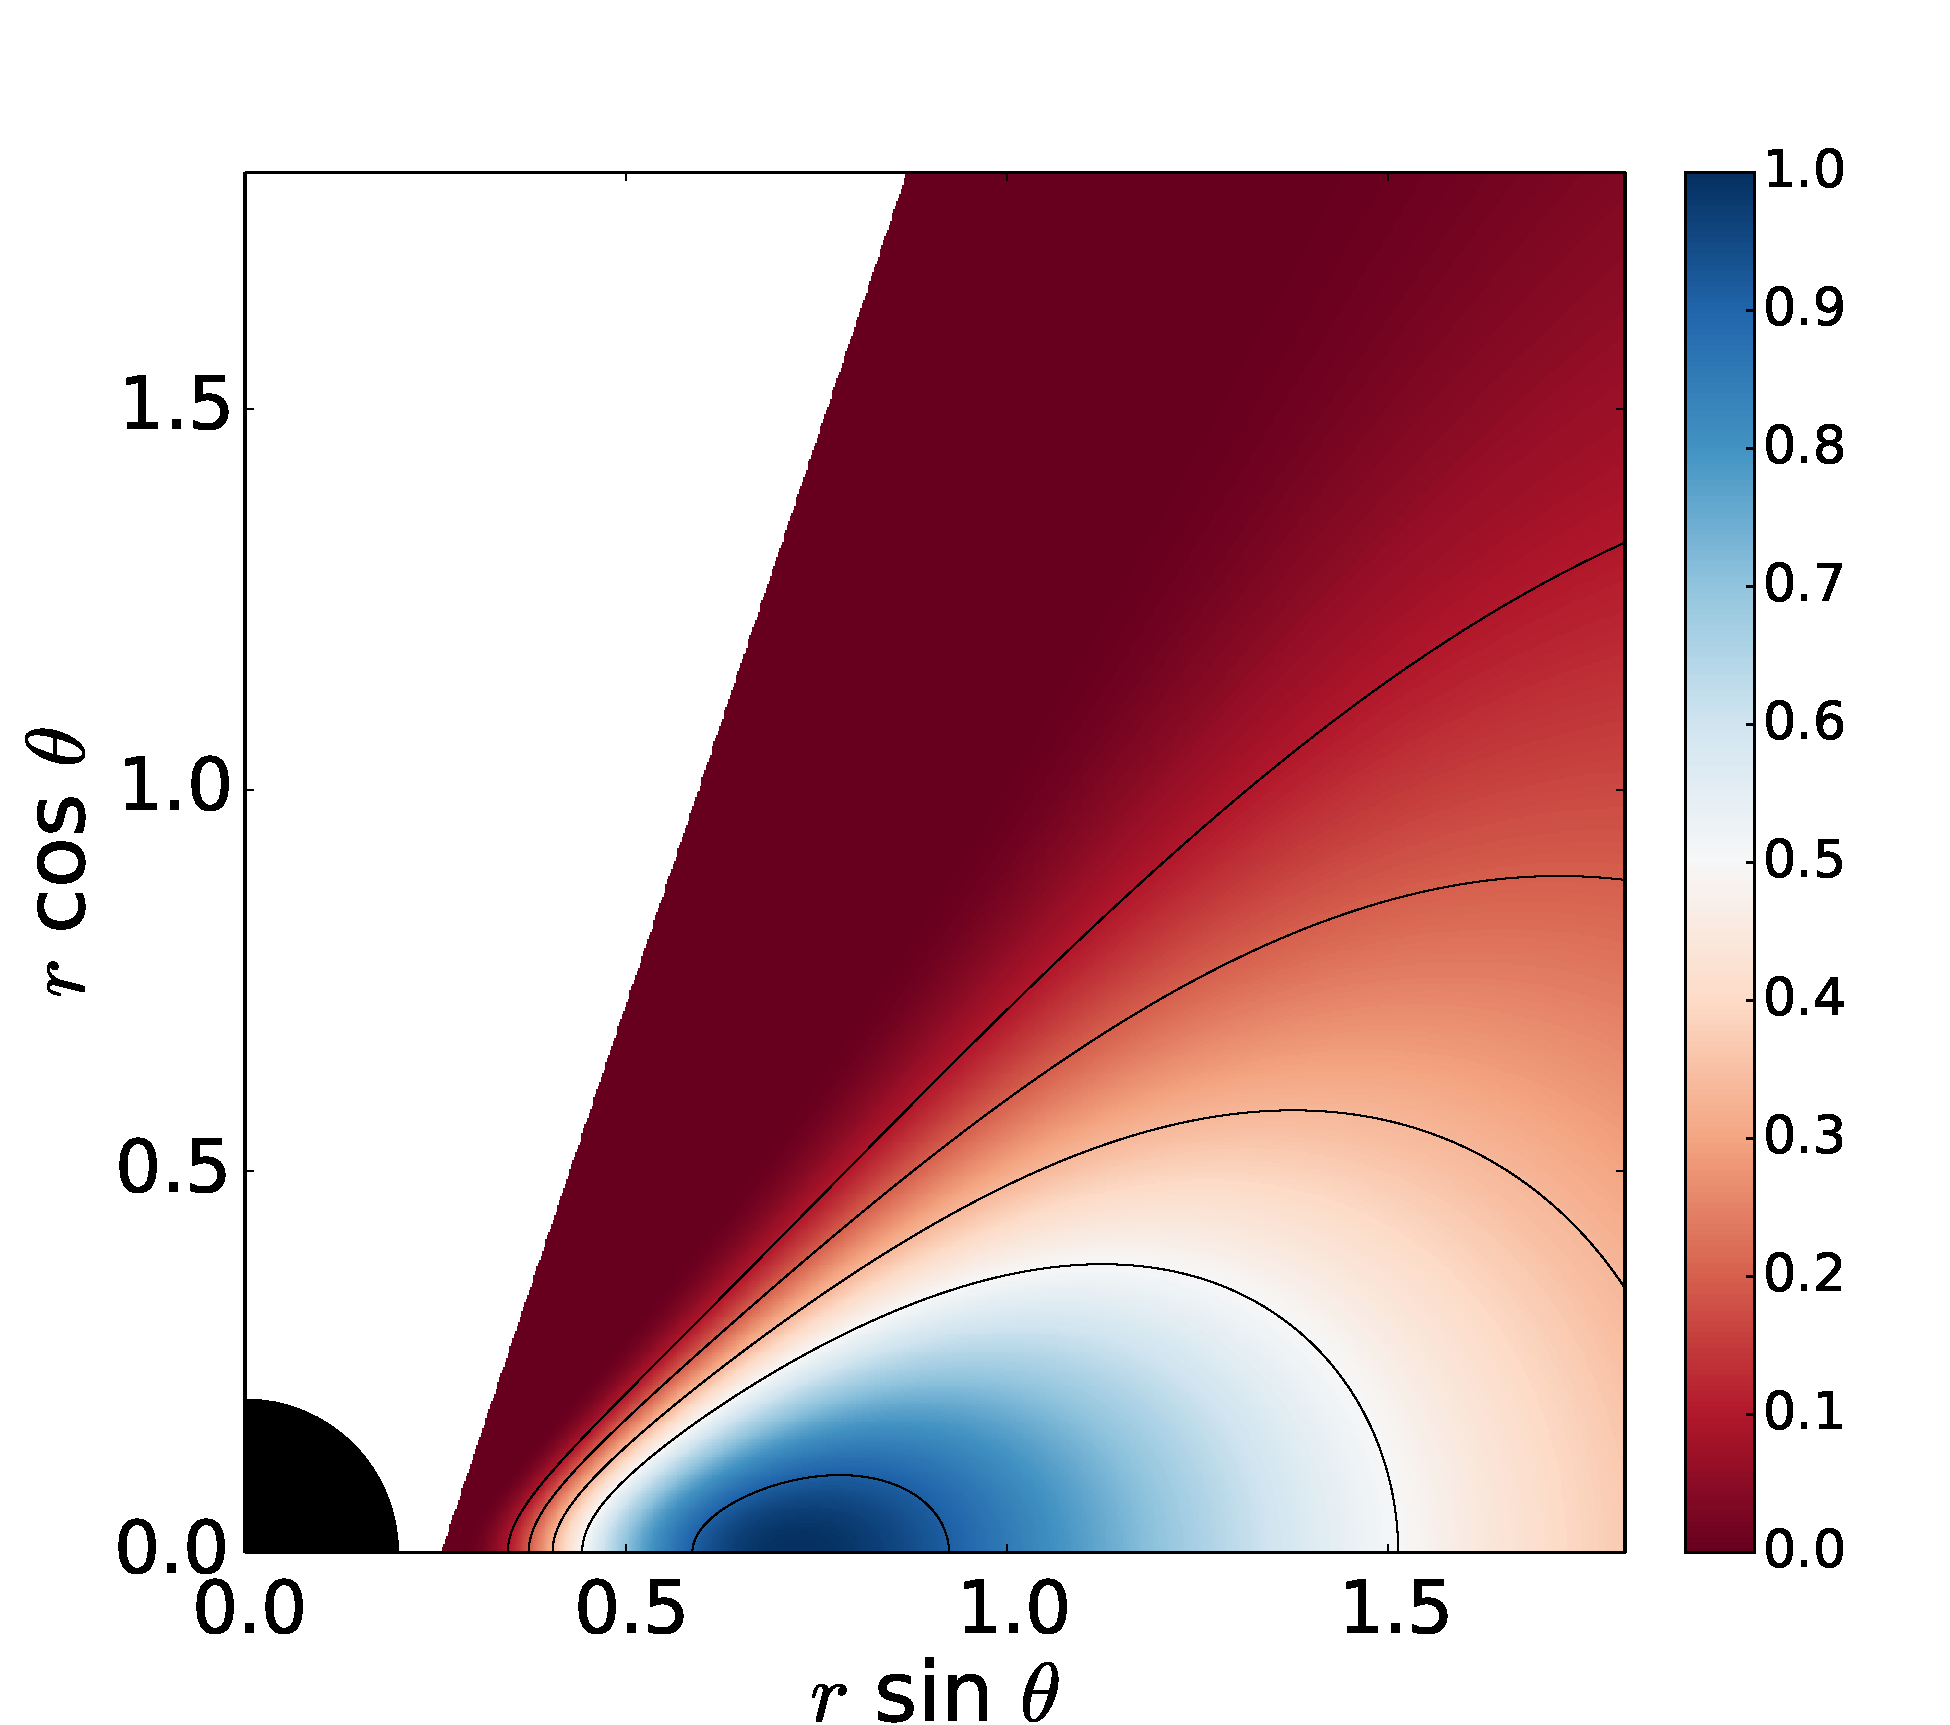
\includegraphics[scale=0.2]{figures/fig2_III_HBH_3.pdf}
\hspace{-0.3cm}
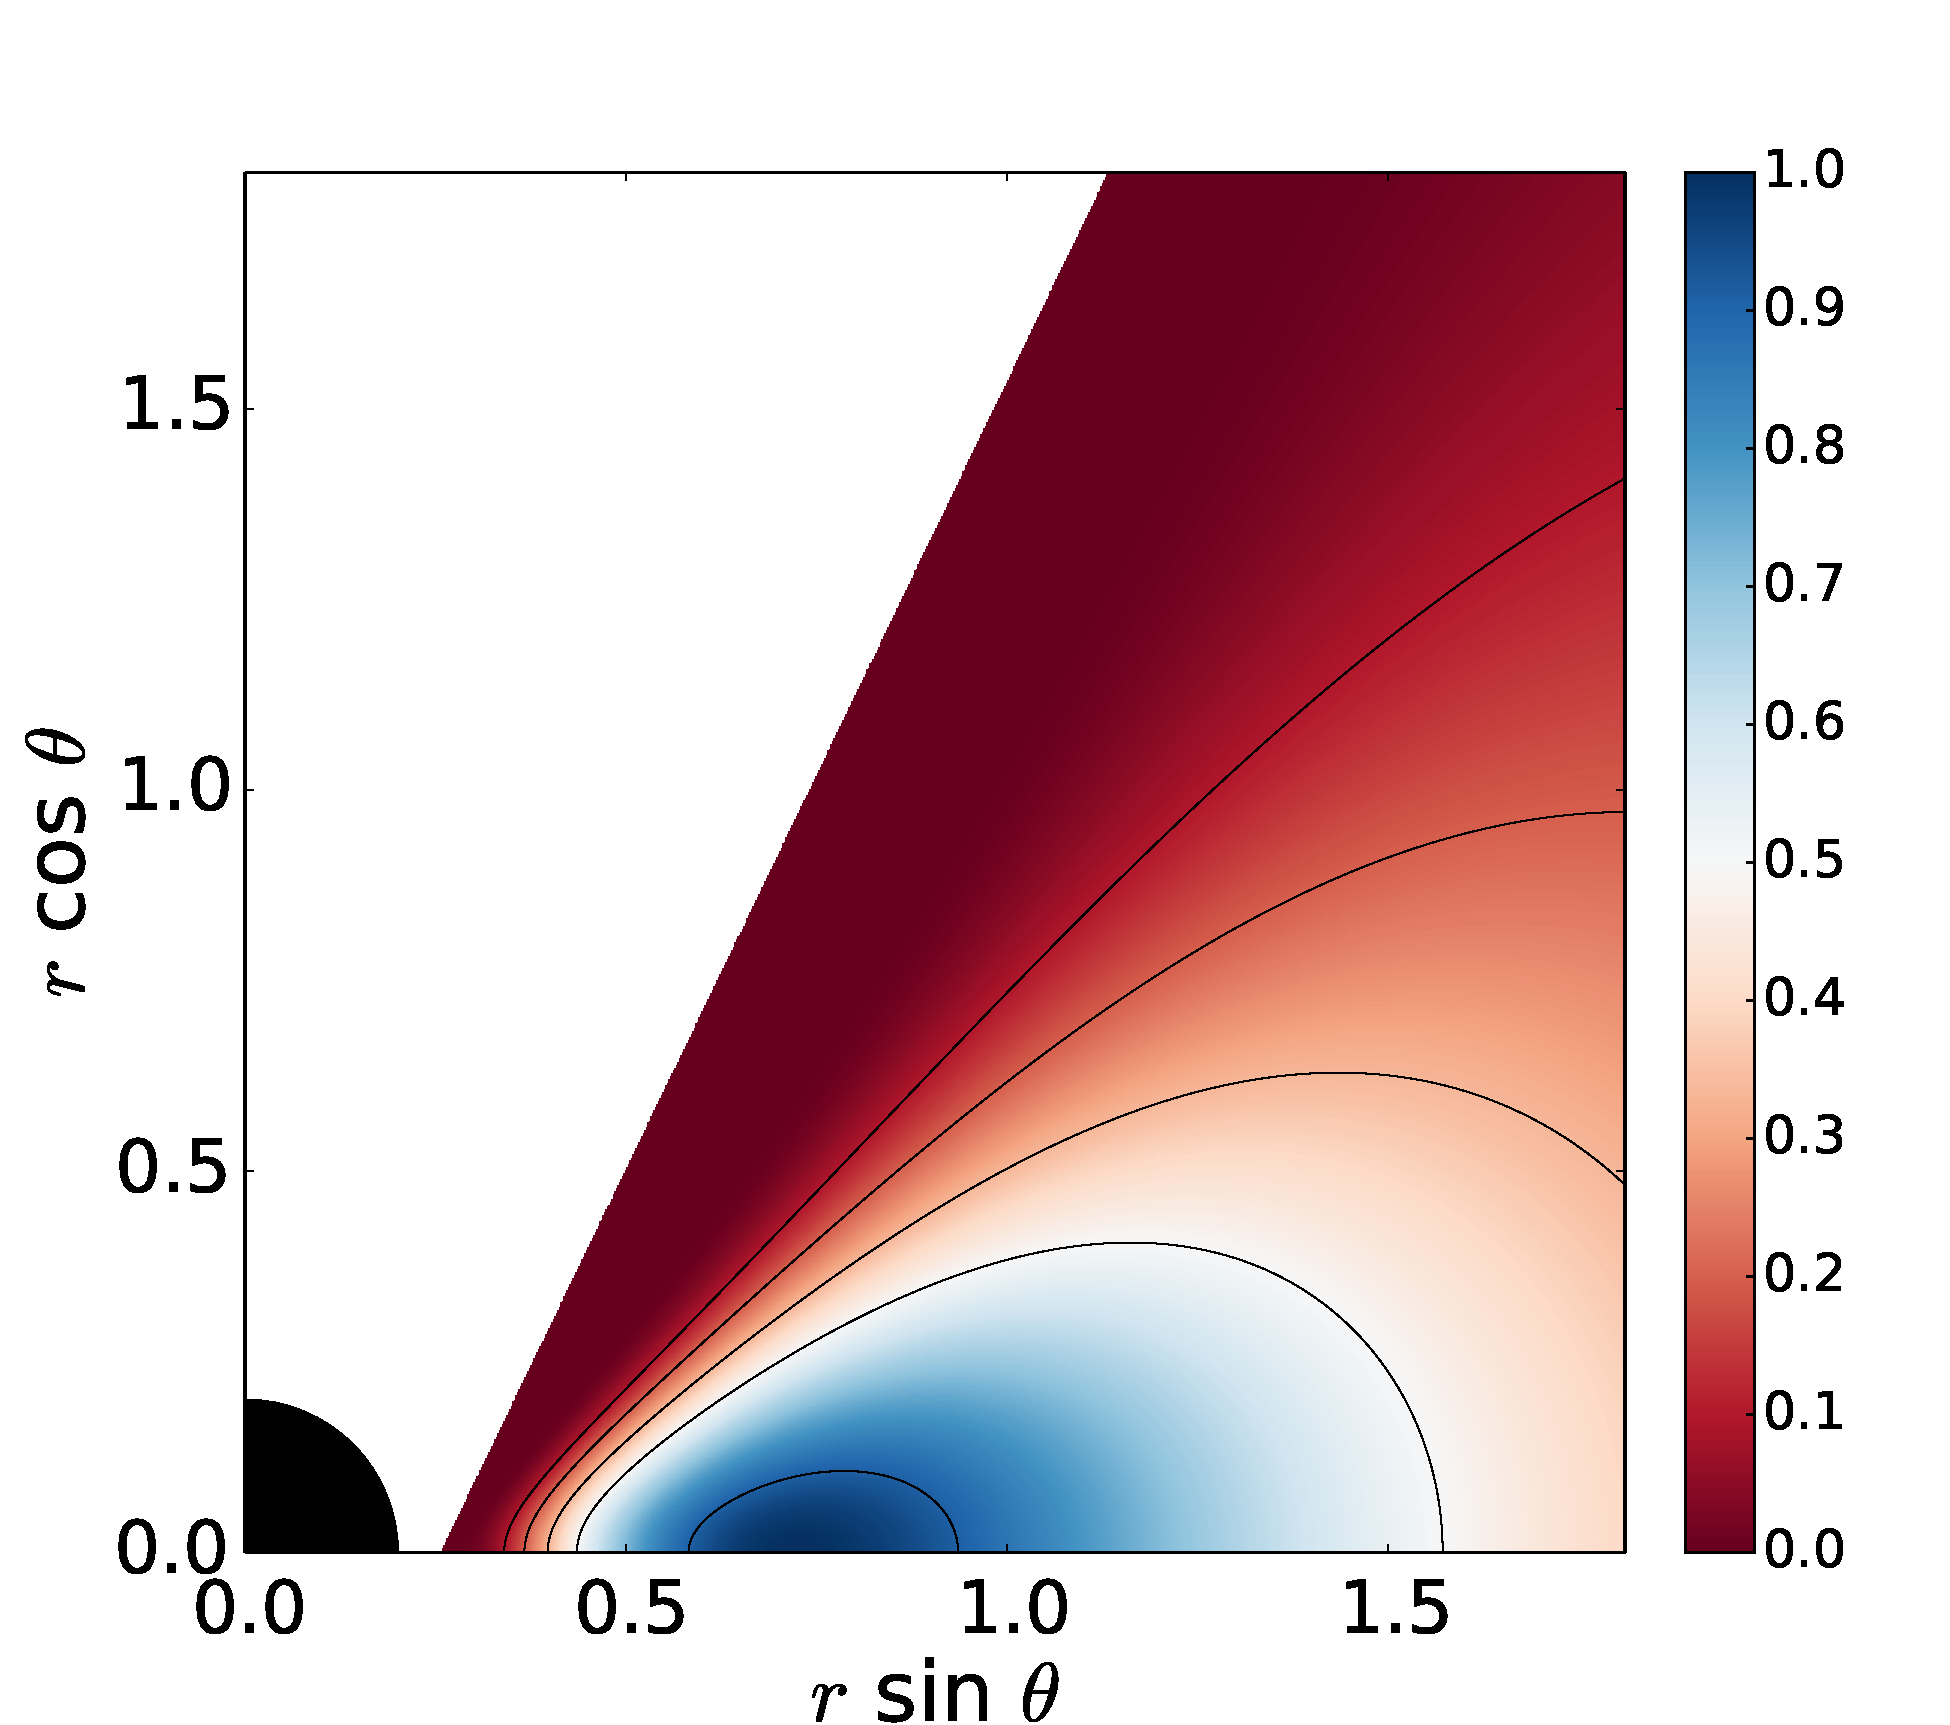
\includegraphics[scale=0.2]{figures/fig2_III_K_3.pdf}
\hspace{-0.2cm}
\\
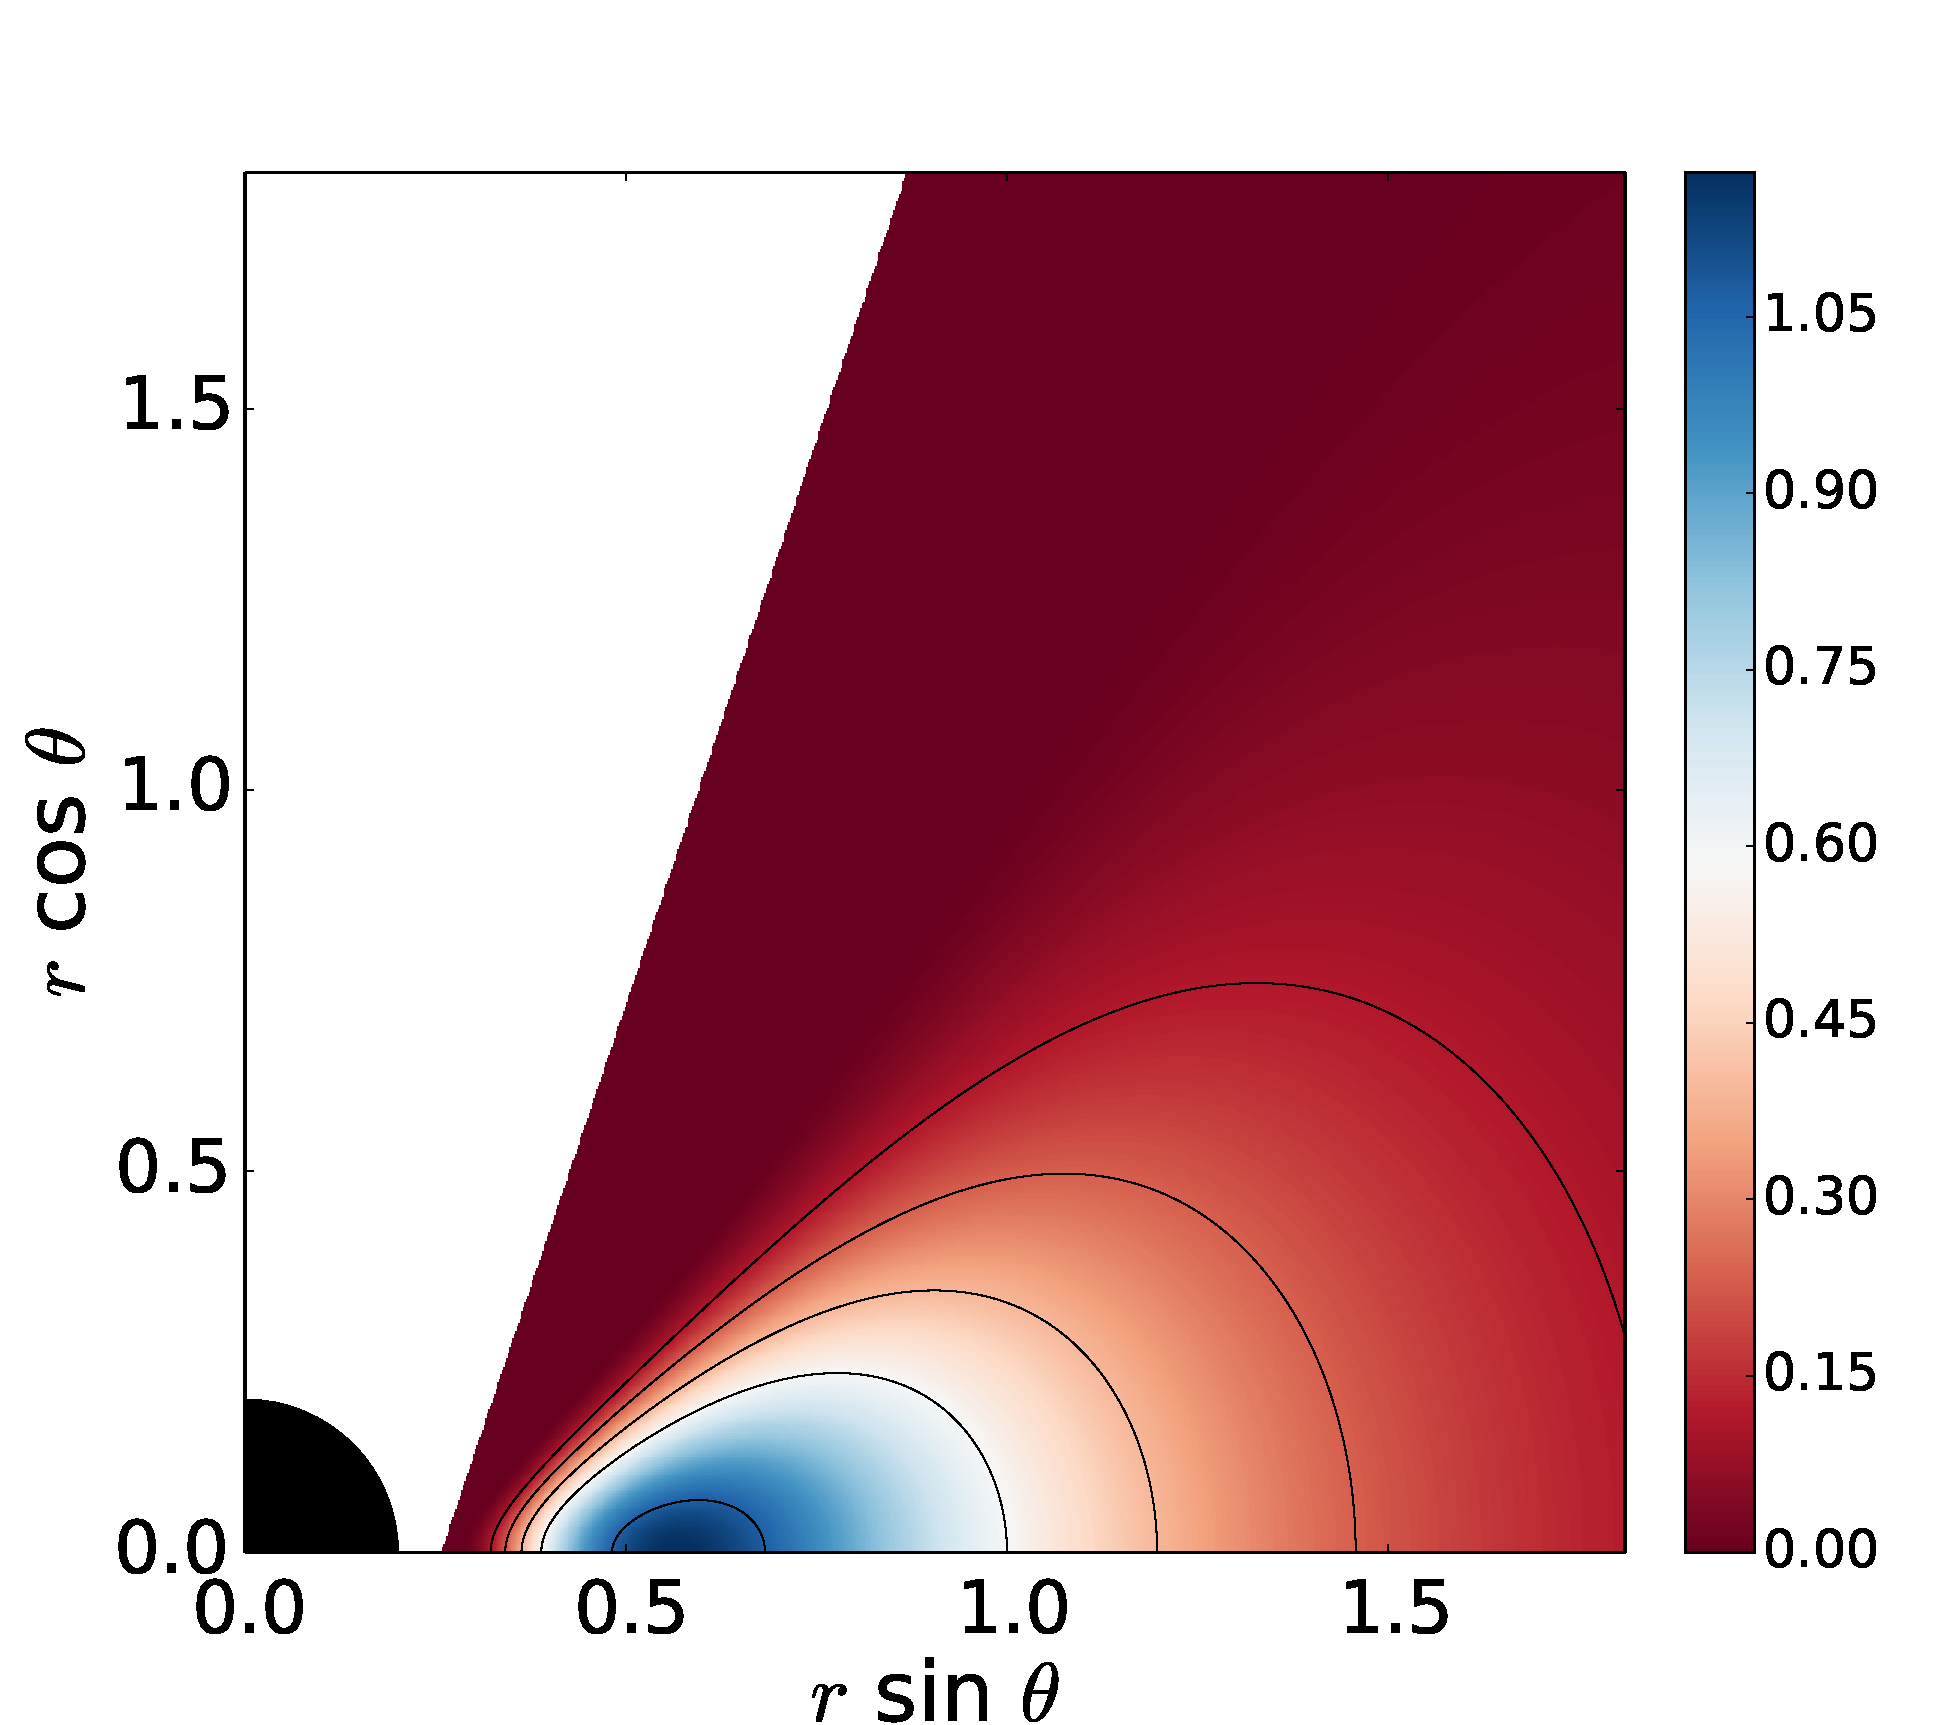
\includegraphics[scale=0.2]{figures/fig2_III_HBH_0.pdf}
\hspace{-0.3cm}
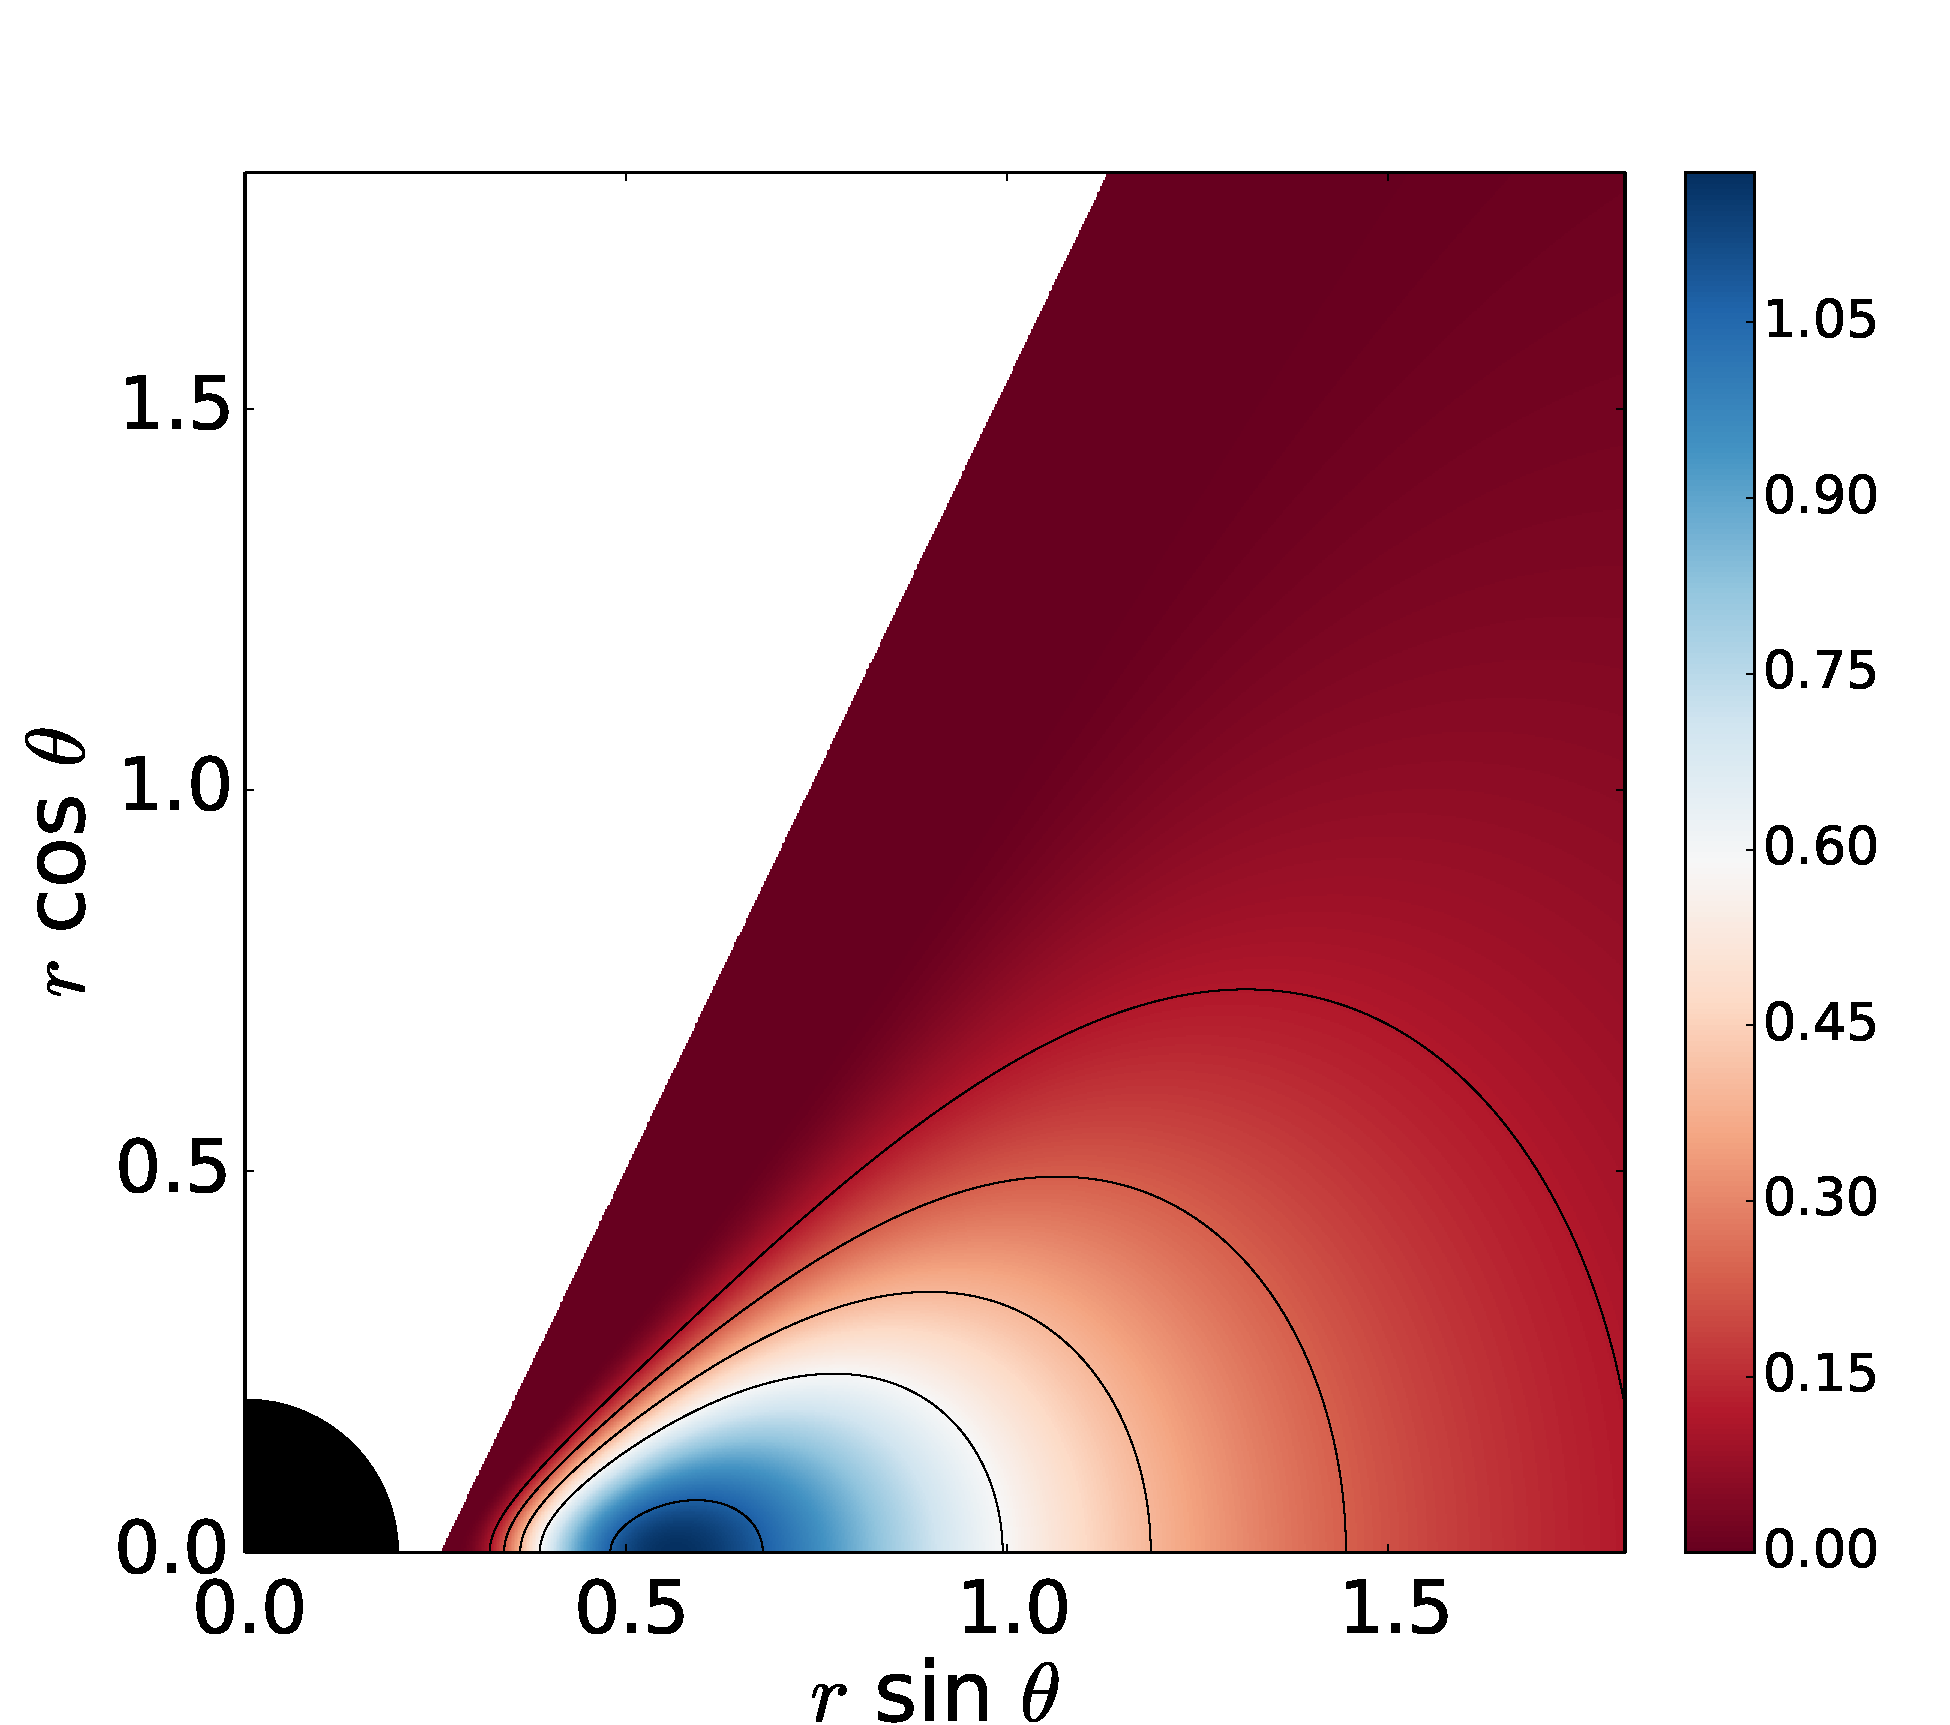
\includegraphics[scale=0.2]{figures/fig2_III_K_0.pdf}
\hspace{-0.2cm}
\\
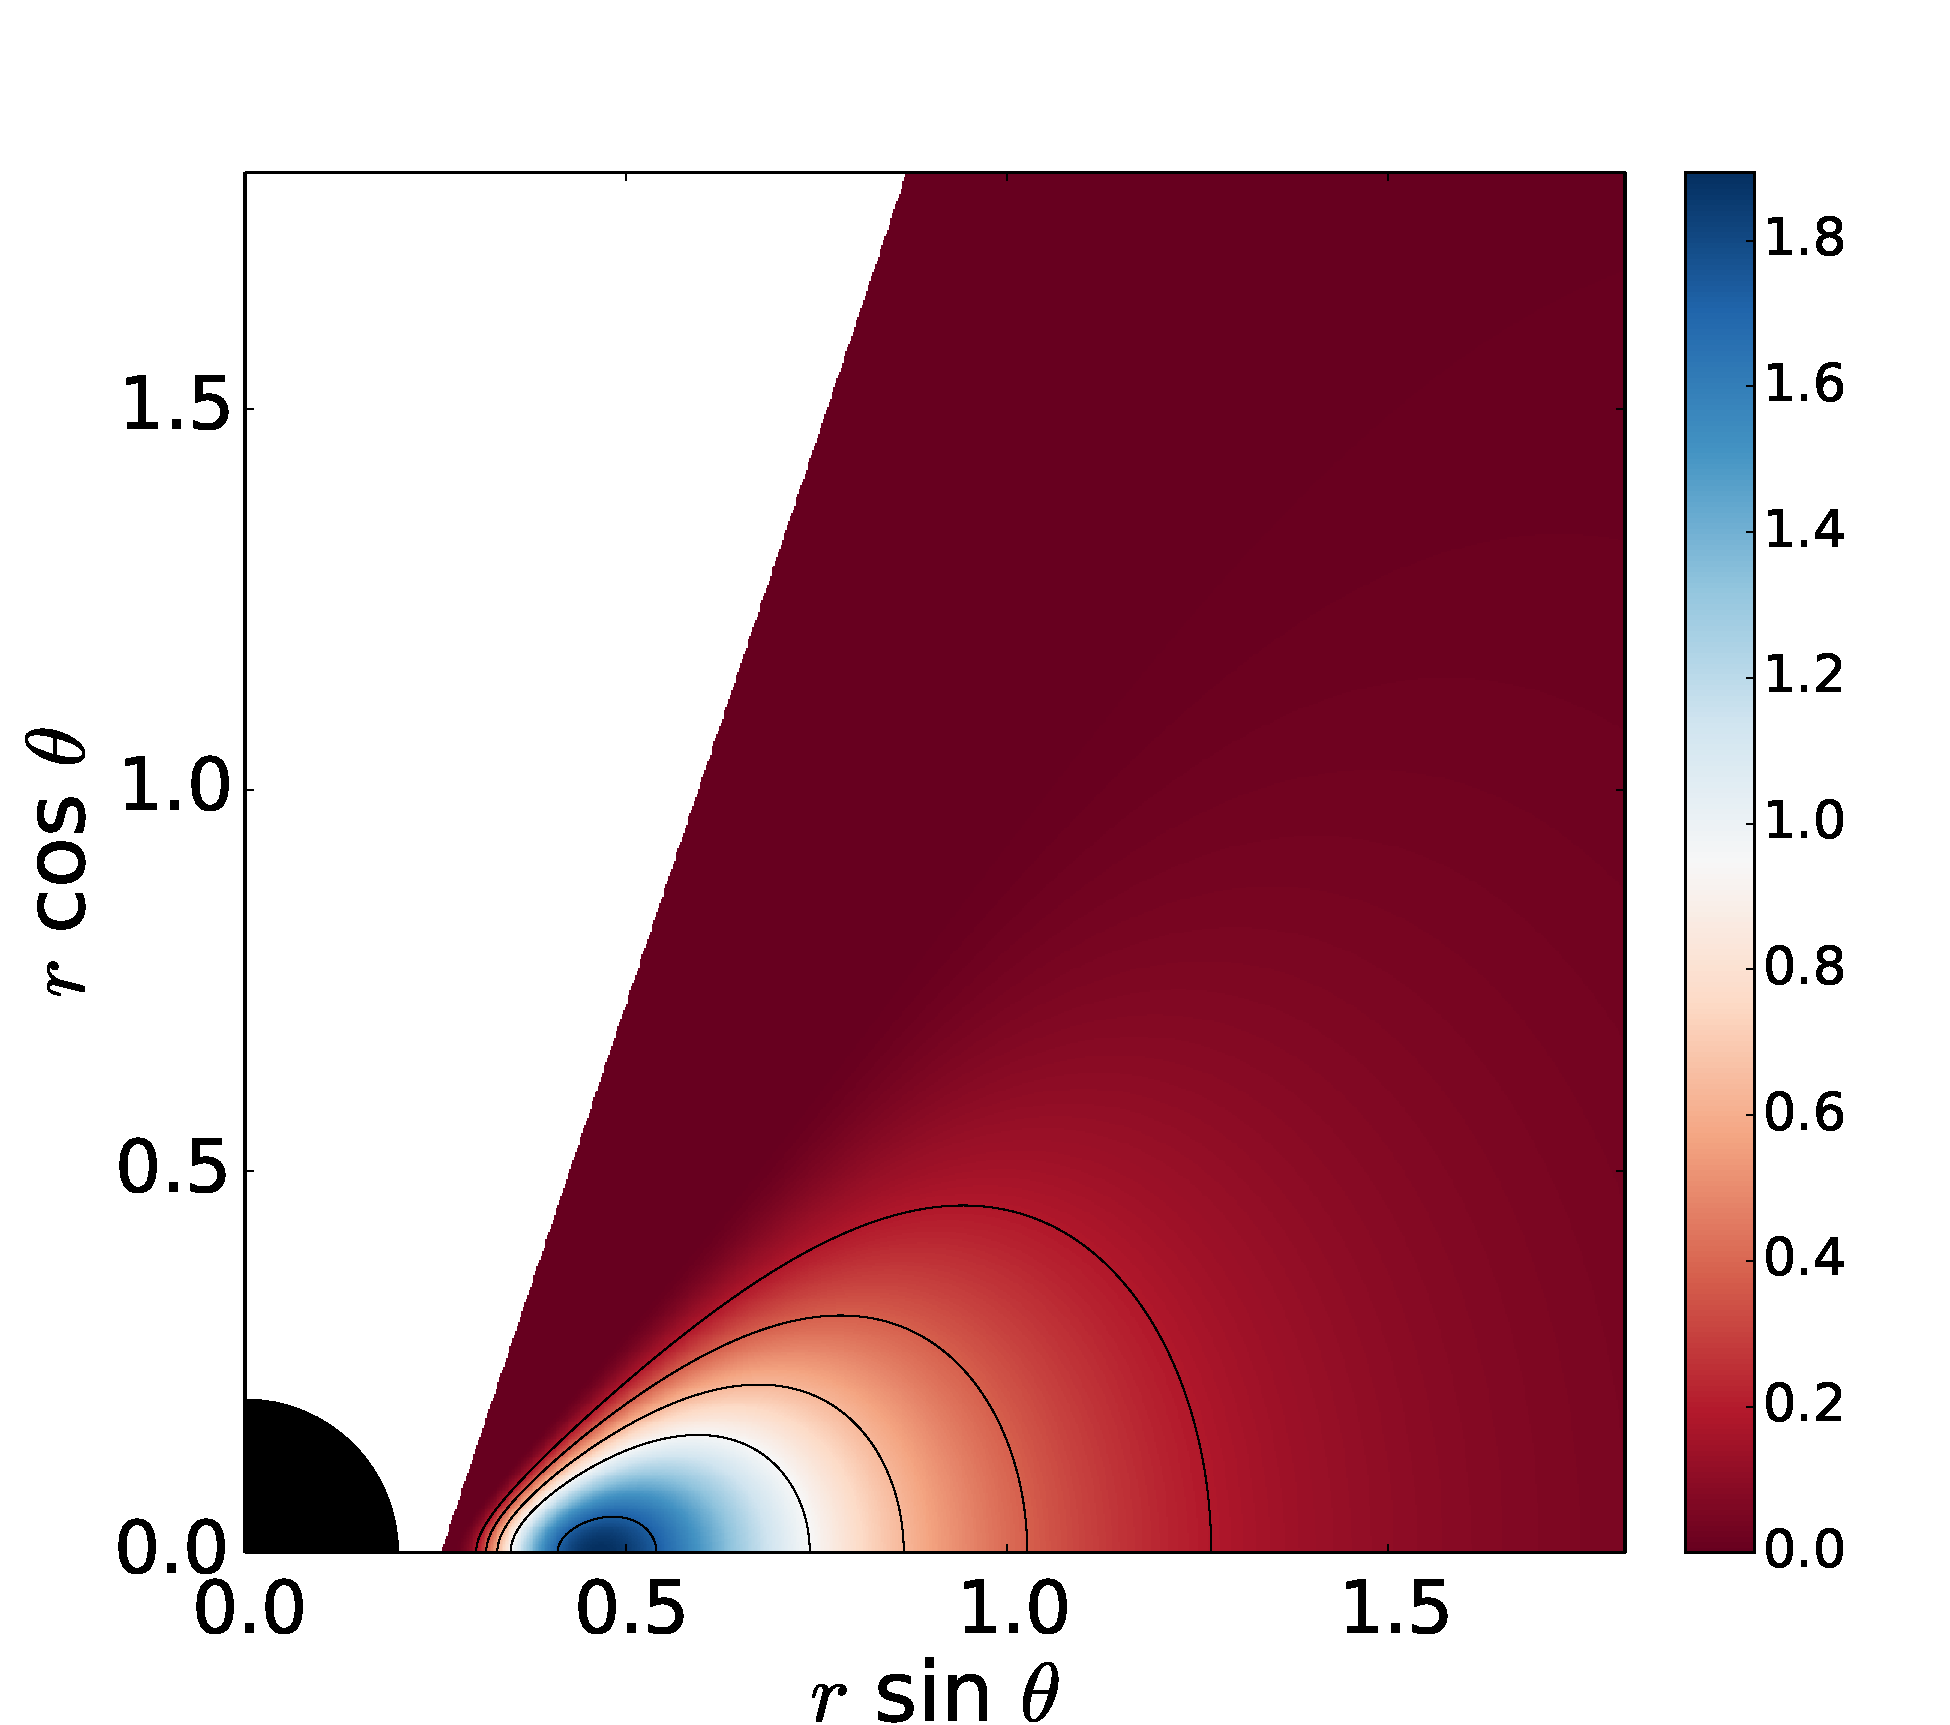
\includegraphics[scale=0.2]{figures/fig2_III_HBH__3.pdf}
\hspace{-0.3cm}
\includegraphics[scale=0.2]{figures/fig2_III_K__3.pdf}
\hspace{-0.2cm}
\caption{Rest-mass density distribution for the model I. From top to bottom the rows correspond to the different values of the magnetization parameter, namely non-magnetized ($\beta_{\mathrm{m}_{\mathrm{c}}} = 10^{3}$), mildly magnetized ($\beta_{\mathrm{m}_{\mathrm{c}}} = 1$) and strongly magnetized ($\beta_{\mathrm{m}_{\mathrm{c}}} = 10^{-3}$). The left column correspond to the KBHsSH model using~\citet{Montero:2007} and the right column correspond to the~\citet{Komissarov:2006} approximation.}
\label{comparison_alt_mag_1}
\end{figure*}

\begin{figure*}
\centering
\includegraphics[scale=0.2]{figures/fig3_IV_HBH_3.pdf}
\hspace{-0.3cm}
\includegraphics[scale=0.2]{figures/fig3_IV_K_3.pdf}
\hspace{-0.2cm}
\\
\includegraphics[scale=0.2]{figures/fig3_IV_HBH_0.pdf}
\hspace{-0.3cm}
\includegraphics[scale=0.2]{figures/fig3_IV_K_0.pdf}
\hspace{-0.2cm}
\\
\includegraphics[scale=0.2]{figures/fig3_IV_HBH__3.pdf}
\hspace{-0.3cm}
\includegraphics[scale=0.2]{figures/fig3_IV_K__3.pdf}
\hspace{-0.2cm}
\caption{Rest-mass density distribution for the model II. From top to bottom the rows correspond to the different values of the magnetization parameter, namely non-magnetized ($\beta_{\mathrm{m}_{\mathrm{c}}} = 10^{3}$), mildly magnetized ($\beta_{\mathrm{m}_{\mathrm{c}}} = 1$) and strongly magnetized ($\beta_{\mathrm{m}_{\mathrm{c}}} = 10^{-3}$). The left column correspond to the KBHsSH model using~\citet{Montero:2007} and the right column correspond to the~\citet{Komissarov:2006} approximation.}
\label{comparison_alt_mag_2}
\end{figure*}

\begin{figure*}
\centering
\includegraphics[scale=0.2]{figures/fig4_V_HBH_3.pdf}
\hspace{-0.3cm}
\includegraphics[scale=0.2]{figures/fig4_V_K_3.pdf}
\hspace{-0.2cm}
\\
\includegraphics[scale=0.2]{figures/fig4_V_HBH_0.pdf}
\hspace{-0.3cm}
\includegraphics[scale=0.2]{figures/fig4_V_K_0.pdf}
\hspace{-0.2cm}
\\
\includegraphics[scale=0.2]{figures/fig4_V_HBH__3.pdf}
\hspace{-0.3cm}
\includegraphics[scale=0.2]{figures/fig4_V_K__3.pdf}
\hspace{-0.2cm}
\caption{Rest-mass density distribution for the model III. From top to bottom the rows correspond to the different values of the magnetization parameter, namely non-magnetized ($\beta_{\mathrm{m}_{\mathrm{c}}} = 10^{3}$), mildly magnetized ($\beta_{\mathrm{m}_{\mathrm{c}}} = 1$) and strongly magnetized ($\beta_{\mathrm{m}_{\mathrm{c}}} = 10^{-3}$). The left column correspond to the KBHsSH model using~\citet{Montero:2007} and the right column correspond to the~\citet{Komissarov:2006} approximation.}
\label{comparison_alt_mag_3}
\end{figure*}

\begin{figure*}
\centering
\includegraphics[scale=0.3]{figures/radial_III_HBH_3.pdf}
\hspace{-0.3cm}
\includegraphics[scale=0.3]{figures/radial_III_K_3.pdf}
\hspace{-0.2cm}
\\
\includegraphics[scale=0.3]{figures/radial_III_HBH_0.pdf}
\hspace{-0.3cm}
\includegraphics[scale=0.3]{figures/radial_III_K_0.pdf}
\hspace{-0.2cm}
\\
\includegraphics[scale=0.3]{figures/radial_III_HBH__3.pdf}
\hspace{-0.3cm}
\includegraphics[scale=0.3]{figures/radial_III_K__3.pdf}
\hspace{-0.2cm}
\caption{Radial rest-mass density distribution for the model I at the equatorial plane. From top to bottom the rows correspond to the different values of the magnetization parameter, namely non-magnetized ($\beta_{\mathrm{m}_{\mathrm{c}}} = 10^{3}$), mildly magnetized ($\beta_{\mathrm{m}_{\mathrm{c}}} = 1$) and strongly magnetized ($\beta_{\mathrm{m}_{\mathrm{c}}} = 10^{-3}$). The left column correspond to the KBHsSH model using~\citet{Montero:2007} and the right column correspond to the~\citet{Komissarov:2006} approximation.}
\label{comparison_alt_radial_1}
\end{figure*}

\begin{figure*}
\centering
\includegraphics[scale=0.3]{figures/radial_IV_HBH_3.pdf}
\hspace{-0.3cm}
\includegraphics[scale=0.3]{figures/radial_IV_K_3.pdf}
\hspace{-0.2cm}
\\
\includegraphics[scale=0.3]{figures/radial_IV_HBH_0.pdf}
\hspace{-0.3cm}
\includegraphics[scale=0.3]{figures/radial_IV_K_0.pdf}
\hspace{-0.2cm}
\\
\includegraphics[scale=0.3]{figures/radial_IV_HBH__3.pdf}
\hspace{-0.3cm}
\includegraphics[scale=0.3]{figures/radial_IV_K__3.pdf}
\hspace{-0.2cm}
\caption{Radial rest-mass density distribution for the model II at the equatorial plane. From top to bottom the rows correspond to the different values of the magnetization parameter, namely non-magnetized ($\beta_{\mathrm{m}_{\mathrm{c}}} = 10^{3}$), mildly magnetized ($\beta_{\mathrm{m}_{\mathrm{c}}} = 1$) and strongly magnetized ($\beta_{\mathrm{m}_{\mathrm{c}}} = 10^{-3}$). The left column correspond to the KBHsSH model using~\citet{Montero:2007} and the right column correspond to the~\citet{Komissarov:2006} approximation.}
\label{comparison_alt_radial_2}
\end{figure*}

\begin{figure*}
\centering
\includegraphics[scale=0.3]{figures/radial_V_HBH_3.pdf}
\hspace{-0.3cm}
\includegraphics[scale=0.3]{figures/radial_V_K_3.pdf}
\hspace{-0.2cm}
\\
\includegraphics[scale=0.3]{figures/radial_V_HBH_0.pdf}
\hspace{-0.3cm}
\includegraphics[scale=0.3]{figures/radial_V_K_0.pdf}
\hspace{-0.2cm}
\\
\includegraphics[scale=0.3]{figures/radial_V_HBH__3.pdf}
\hspace{-0.3cm}
\includegraphics[scale=0.3]{figures/radial_V_K__3.pdf}
\hspace{-0.2cm}
\caption{Radial rest-mass density distribution for the model III at the equatorial plane. From top to bottom the rows correspond to the different values of the magnetization parameter, namely non-magnetized ($\beta_{\mathrm{m}_{\mathrm{c}}} = 10^{3}$), mildly magnetized ($\beta_{\mathrm{m}_{\mathrm{c}}} = 1$) and strongly magnetized ($\beta_{\mathrm{m}_{\mathrm{c}}} = 10^{-3}$). The left column correspond to the KBHsSH model using~\citet{Montero:2007} and the right column correspond to the~\citet{Komissarov:2006} approximation.}
\label{comparison_alt_radial_3}
\end{figure*}
\end{appendix}

\end{document}
